\documentclass[12pt,a4paper]{report}

\usepackage[ngerman,provide=*]{babel}
\usepackage[T1]{fontenc}
\usepackage{lmodern}
\usepackage{amsmath,amssymb,graphicx}
\usepackage{geometry}
\geometry{margin=2.5cm}
\usepackage{placeins}
\usepackage{booktabs,array,longtable}
\setlength{\emergencystretch}{3em}
\hyphenation{Elek-tro-ma-gne-ti-sche Schwin-gungs-kopp-lung}
\usepackage[hidelinks,unicode]{hyperref}
\hypersetup{
  pdftitle={Wellenformstatistik der unilateralen Kontaktkraft in phasenkontrollierten Mehrmassensystemen},
  pdfauthor={Matthias Früh},
  pdfsubject={PCMMS -- Prä-experimentelles Arbeitspapier, Version 2.3},
  pdfkeywords={PCMMS, Kontaktkraft, Wellenformstatistik, Phasensteuerung, Arbeitspapier}
}

\begin{document}

\begin{titlepage}
\thispagestyle{empty}
\centering
\vspace*{1.2cm}
{\Large\textsc{PCMMS}}\\[0.3cm]
{\large Phase-Controlled Multi-Mass Systems}\\[1.5cm]
{\Large\textsc{Arbeitspapier}}\\[1.0cm]
{\LARGE\bfseries
Wellenformstatistik der unilateralen Kontaktkraft\\[0.3cm]
in phasenkontrollierten Mehrmassensystemen
\par}
\vspace{0.8cm}
{\large Messrahmen, numerische Referenzfälle und Artefaktkontrolle\par}
\vspace{1.5cm}
{\Large\textbf{Matthias Früh}}\\[0.4cm]
{\normalsize Unabhängiges Forschungsvorhaben}\\[0.3cm]
{\normalsize ORCID: \href{https://orcid.org/0009-0005-9984-4207}{0009-0005-9984-4207}}
\vfill
\begin{minipage}{0.9\textwidth}
\centering
Prä-experimenteller Arbeitsstand\\[0.3cm]
Version 2.3 -- 25. September 2026\\[0.6cm]
\small
Korrigierte Fassung: Basislinienresiduum als Randterm des Auswertefensters.\\
Numerische Ergebnisse und Messkonzept; eigene experimentelle Nachweise stehen aus.
\end{minipage}
\vspace*{0.7cm}
\end{titlepage}

\pagenumbering{roman}
\tableofcontents
\clearpage

\chapter*{Kurzfassung}
\addcontentsline{toc}{chapter}{Kurzfassung}

Die Arbeit entwickelt einen Messrahmen für die Kontaktkraft eines
geschlossenen Körpers, dessen drei innere Massen phasengesteuert
periodisch bewegt werden und dessen Auflage einseitig ist, also innerhalb
eines Zyklus abheben kann. Sie ist prä-experimentell: Der Aufbau ist
ausgelegt, nicht gebaut; alle Zahlenwerte stammen aus Simulationen.

Ausgangspunkt ist eine Einschränkung, keine Hypothese. Der
Schwerpunktsatz legt das Zeitmittel der Kontaktkraft für jede innere
Konfiguration auf $Mg$ fest. Eine zustandsabhängige Differenz
zeitgemittelter Kräfte ist deshalb als Effektgröße nicht verfügbar; eine
frühere Phase des Projekts, die eine solche Differenz berichtet hatte,
wurde zurückgezogen. Der Rahmen kehrt die Rolle dieser Größe um: Ihr
wahrer Wert ist bekannt, und sie dient als In-situ-Kontrolle der
vollständigen Auswertekette. Die Zielgrößen sind Funktionale der
Wellenform --- Schiefe, Liftoff-Anteil, Asymmetrieverhältnis, minimale
Kontaktkraft ---, die der Erhaltungssatz frei lässt. Die Auswertung ist
zweispurig: erst Qualifikation der Apparatur gegen die bekannte
Nullgröße, dann Prüfung der Zielgrößen gegen eine aus der
Wiederholpräzision bestimmte Schwelle. Sie folgt einer Äquivalenzlogik --- ein
Nullergebnis wird durch ein Intervall innerhalb der Schwelle
nachgewiesen, nicht aus fehlender Signifikanz geschlossen --- und endet
in genau einem von vier Zuständen: Apparaturfehler, unbestimmt,
nachgewiesenes Nullergebnis mit oberer Schranke, nachgewiesene
Abhängigkeit ohne Mechanismusbehauptung.

Die Simulationsstudie über ein $19\times19$-Raster der relativen Phasen
liefert vier Befunde, die den Aufbau binden. Das Residuum gegen die
Basislinie liegt bei Dauerkontakt bei $0{,}2\,\mathrm{ppm}$. Größere Werte
--- im Archivlauf bis $0{,}68\,\%$, nach adaptivem Burn-in bis
$0{,}37\,\%$ --- sind kein Fehler der Integration, deren Anteil unter
$0{,}01\,\%$ bleibt, sondern ein Randterm des Auswertefensters: die
Änderung der Schwerpunktsgeschwindigkeit über das Fenster, bezogen auf
$g$ und Fensterlänge. Er entsteht bei unvollständigem Einschwingen, bei
Fenstern ohne ganze Orbitperioden und bei aperiodischer Bewegung, fällt
mit der Fensterlänge ab, kann als phasenabhängiger Effekt erscheinen und
ist die quantitative Signatur des zurückgezogenen Befunds. Die vier
Funktionale sind nicht unabhängig; nur die minimale Kontaktkraft trägt
eigenständige Information. Negative Schiefe tritt nur auf, wenn kein
Modulpaar gleichphasig läuft --- eine mit drei Messungen prüfbare
Vorhersage, nach Stichproben gültig in einem Bereich der
Kontaktsteifigkeit und -dämpfung. Und mit sinusförmigem Antrieb kollabiert die gesamte
Phasenkarte auf die resultierende Amplitude: Die Asymmetrie des
Bahnprofils ist die Quelle der Phasenabhängigkeit, ein Antrieb mit
asymmetrischem Profil zwingend.

Die Grenze des Rahmens wird benannt. Die Kontrolle prüft das erste
Moment; phasenkorrelierte Einkopplung, symmetrische Kettenfehler und
amplitudenabhängige Kennlinien bestehen sie und verfälschen dennoch die
Wellenform. Sie sind nur durch Versuchsanordnung zu behandeln, vor allem
durch Leerläufe mit bestromter, aber blockierter Aktuierung.

Die Arbeit behauptet keine neue Physik. Ihr Beitrag ist methodisch und
eng: die Verwendung einer erhaltungsgarantierten Nullgröße als Prüfmittel
gegen die eigene Messkette, und die Wellenform der Kontaktkraft als
entworfene Zielgröße einer Phasensteuerung innerer Massen.

\clearpage

\chapter*{Abstract}
\addcontentsline{toc}{chapter}{Abstract}

This working paper develops a measurement framework for the contact force of a
closed body whose three internal masses are driven periodically under
phase control and whose support is unilateral, so that contact may be
lost within a cycle. The work is pre-experimental: the apparatus is
designed, not built, and all numerical values are simulated.

The starting point is a constraint rather than a hypothesis. The
centre-of-mass theorem fixes the time-averaged contact force at $Mg$ for
every internal configuration; a state-dependent difference of
time-averaged forces is therefore unavailable as an effect quantity, and
an earlier project stage that had reported one has been withdrawn. The
framework inverts the role of this quantity: its true value is known,
and it serves as an in-situ control of the complete evaluation chain.
The target quantities are functionals of the waveform --- skewness,
liftoff fraction, asymmetry ratio, minimum contact force --- which the
conservation law leaves free. Evaluation proceeds on two tracks,
apparatus qualification against the known null before target evaluation
against a threshold derived from reference repeatability, and
follows an equivalence logic --- a null result is established by an
interval lying within the threshold, not inferred from absent
significance --- and terminates in one of four states: apparatus fault,
undetermined, established null result with an upper bound, or detected
dependence without a claimed mechanism.

A simulation study over a $19\times19$ grid of relative phases yields
four findings that bind the design. The residual against the baseline
is $0{.}2\,\mathrm{ppm}$ under permanent contact. Larger values --- up to
$0{.}68\,\%$ in the archived run and up to $0{.}37\,\%$ after adaptive
burn-in --- are not an integration error, whose share stays below
$0{.}01\,\%$, but a boundary term of the evaluation window: the change of
the centre-of-mass velocity across the window, divided by $g$ times the
window length. It arises from incomplete transients, from windows not
spanning whole orbit periods and from aperiodic motion, decays with
window length, can masquerade as a phase-dependent effect and is the
quantitative signature of the withdrawn result. The four functionals are not
independent; only the minimum contact force carries separate
information. Negative skewness occurs only when no pair of modules is in
phase --- a prediction testable with three measurements, valid --- on the basis of
sampled cases --- within a range of contact stiffness and damping. With sinusoidal drive the
entire phase map collapses onto the resultant amplitude: the asymmetry
of the motion profile is the source of the phase dependence, and a drive
producing an asymmetric profile is mandatory.

The limit of the framework is stated. The control tests the first
moment; phase-correlated coupling, symmetric chain errors and
amplitude-dependent transfer pass it and still corrupt the waveform.
They are addressed by experimental design, above all by idle runs with
energised but blocked actuation.

No new physics is claimed. The contribution is methodological and
narrow: the use of a conservation-guaranteed null as a check on one's
own measurement chain, and the contact-force waveform as the designed
target of phase control over internal masses.

\clearpage

\pagenumbering{arabic}

%======
\chapter*{Status und Versionshinweis}
\addcontentsline{toc}{chapter}{Status und Versionshinweis}

Dieses Arbeitspapier dokumentiert den prä-experimentellen Forschungsstand
von PCMMS zur phasen- und profilgesteuerten Mehrmassendynamik. Es umfasst
einen theoretischen und messtechnischen Rahmen, numerische Referenzfälle
sowie ein vorgeschlagenes Prüf- und Auswerteverfahren. Eigene
experimentelle Nachweise stehen aus. Simulationsbefunde sind an die
jeweiligen Modellannahmen, Parameter und Auswertefenster gebunden.

Die Fassung v2.2 geht aus dem Arbeitsmanuskript v2.1 hervor, das bisher
unter der Bezeichnung \emph{Dissertation} geführt wurde. Sie wird hier
als eigenständiges Arbeitspapier vorgelegt. Die früheren Platzhalter für
Hochschule, akademischen Grad und Betreuung sowie die promotionsbezogene
Erklärung sind entfallen. Mit dieser Fassung ist keine Einreichung als
Promotionsschrift verbunden.

Die Überarbeitung zu v2.2 betrifft die Dokumentbezeichnung, das Titelblatt,
diesen Versionshinweis, die englische Selbstbezeichnung im Abstract und
die PDF-Metadaten. Tabellenumbrüche und Zeilensatz wurden für die
PDF-Ausgabe angepasst. Der fachliche Haupttext einschließlich der Anhänge,
Formeln und Literaturgrundlage wurde aus v2.1 übernommen. Die dort
bereits enthaltene Zuordnung von $\beta_h$ und die Ergänzungen zum
Feinsweep bleiben bestehen. Das separate Symbol- und Formelverzeichnis
v2.5 bleibt unverändert.

Die Fassung v2.3 vom 25.~September 2026 korrigiert die Deutung des
Basislinienresiduums in Kurzfassung, Abstract,
Abschnitt~\ref{sec:abtaststrategie}, Abschnitt~\ref{sec:track1-sim},
Abschnitt~\ref{sec:sim-zeigt}, Abschnitt~\ref{sec:befunde} und in den
Anhängen~\ref{sec:anh-datensatz}, \ref{sec:anh-residuum} und
\ref{sec:anh-numerik}. Frühere Fassungen erklärten große Residuen mit
einer langsamen Modulation und gaben alle $361$ Residuen als negativ an.
Beides trifft nicht zu: Die Vorzeichen sind gemischt, und die großen
Werte sind der Randterm des Auswertefensters nach
Gleichung~\eqref{eq:randterm}, belegt durch eine Nachrechnung mit
adaptivem Burn-in vom 13.~September 2026. Übrige Inhalte sind gegenüber
v2.2 unverändert. Die neuen Symbole stehen im Symbolverzeichnis dieses Papiers und folgen
dem Formelverzeichnis v2.6.

Der in der Arbeit zitierte Repository-Stand 2026-09 ist über
\href{https://doi.org/10.5281/zenodo.22864178}{doi:10.5281/zenodo.22864178}
referenziert. Dieser DOI bezeichnet das Repository-Paket, nicht das
vorliegende Arbeitspapier. Der Quellcode ist unter
\href{https://github.com/matthias-frueh/phase-controlled-multi-mass-systems}{GitHub: matthias-frueh/phase-controlled-multi-mass-systems}
zugänglich. Datensatz, Skripte und Ergebnisnotiz der Nachrechnung vom
13.~September 2026 liegen dem Quellpaket dieser Fassung bei (Ordner
\texttt{nachrechnung\_2026-09-13}); im Repository-Stand 2026-09 sind sie
nicht enthalten.

Die begleitende Liste offener Punkte führt die noch ausstehenden
Projekt- und Versuchsentscheidungen fort. Die Fassungen v2.2 und v2.3 enthalten keine erneute vollständige
Literaturprüfung. v2.3 übernimmt Zahlen aus der genannten Nachrechnung;
Karten und Abbildungen stammen weiterhin aus dem Archivlauf.

\clearpage

\chapter*{Symbolverzeichnis}
\addcontentsline{toc}{chapter}{Symbolverzeichnis}

\begin{longtable}{@{}p{0.20\textwidth}p{0.76\textwidth}@{}}
\textbf{Symbol} & \textbf{Bedeutung} \\ \hline
\endhead

\multicolumn{2}{l}{\emph{Kontaktkraft und Basislinie}} \\
$N(t)$ & Normalkraft an der Auflagefläche \\
$\langle N \rangle$ & Zeitgemittelte Kontaktkraft über ganzzahlig viele Zyklen \\
$M$, $g$ & Gesamtmasse des Systems, Fallbeschleunigung \\
$Mg$ & Erhaltene Basislinie der zeitgemittelten Kontaktkraft \\

\multicolumn{2}{l}{\emph{Wellenformobservablen (Zielgrößen)}} \\
$\gamma_1$ & Schiefe der Kontaktkraftverteilung \\
$\lambda$ & Liftoff-Anteil \\
$A$ & Asymmetrieverhältnis $(N_{\max}-Mg)/(Mg-N_{\min})$ \\
$N_{\min}$, $N_{\max}$ & Minimale und maximale Kontaktkraft \\
$N_{\text{thr}}$ & Operative Kontaktschwelle zur Liftoff-Erkennung \\
$f$, $T$ & Anregungsfrequenz, Anregungsperiode \\
$f_n$ & Kontakteigenfrequenz $\sqrt{k/M}/(2\pi)$ \\
$k$, $c$, $\zeta$ & Kontaktsteifigkeit, Kontaktdämpfung, Dämpfungsgrad \\
$R$ & Resultierende Amplitude $|1+e^{i\varphi_2}+e^{i\varphi_3}|$ bei Sinusprofil \\
$R_c$, $R_c^{\text{qs}}$ & Liftoff-Schwelle bei Sinusprofil, dynamisch und quasistatisch \\
$T$ & Transmissibilität des Kontakts \\

\multicolumn{2}{l}{\emph{Bahnprofil}} \\
$r_{\text{top}}$, $r_{\text{bot}}$ & Amplituden der Halte- und Rückholphase \\
$\beta_h$, $T_{\text{hold}}$ & Halteanteil (Hold-Zeitanteil $T_{\text{hold}}/T$), Haltedauer \\
$\tau_k$ & Zeitverschiebung des Moduls $k$, $\varphi_k/(2\pi f)$ \\
$\ddot{z}_{\text{egg}}$ & Beschleunigung des Bahnprofils \\

\multicolumn{2}{l}{\emph{Messmodell}} \\
$F_{\text{meas}}(t)$ & Gemessenes Kraftsignal \\
$F_{\text{sys}}(t)$ & Beitrag der Systemdynamik \\
$F_{\text{drift}}(t)$ & Zeitabhängiger Driftanteil \\
$C(x,t)$ & Residualbeiträge \\
$\varepsilon(t)$ & Stochastisches Messrauschen \\
$\mathcal{M}$ & Messoperator, $(F_{\text{in}},\theta,t)\mapsto y$ \\
$F_{\text{in}}(t)$ & An der Messschnittstelle wirkende Kraft \\
$g(\cdot)$, $h(\cdot)$, $f(\cdot)$ & Schnittstellen-, Mess- und Entwicklungsabbildung \\
$p$, $\theta$ & Feste Systemparameter, messseitige Parameter \\
$a(\theta,t)$, $b(\theta,t)$ & Wirksamer Verstärkungsfaktor und Offset \\
$\delta F_{\text{eff}}$ & Wirksame Auflösung der Messkette \\
$B$, $f_s$ & Bandbreite, Abtastrate \\
$t_{10-90}$, $f_{99}$ & Anstiegszeit der Kontaktflanke, 99-Prozent-Frequenz \\

\multicolumn{2}{l}{\emph{Kontrollgröße}} \\
$\bar{F}_{A}$, $\bar{F}_{B}$ & Zeitgemittelte Kraft in den Zuständen $A$ und $B$ \\
$\Delta \bar{F}_{\text{Zustand}}$ & Kontrollgröße; wahrer Wert null nach Erhaltungssatz \\
$\Delta \bar{F}^{(i)}_{\text{Zustand}}$ & Kontrollgröße im Lauf $i$ \\
$\mu_{\Delta}$, $\sigma_{\Delta}$ & Mittel und Standardabweichung der laufweisen Kontrollwerte \\
$\delta$ & Relatives Residuum gegen die erhaltene Basislinie \\
$\delta_w$, $\delta_Q$ & Randterm des Auswertefensters, bezogen auf $Mg$, und Quadraturanteil; $\delta = \delta_w + \delta_Q$ \\
$\Delta v_S$ & Änderung der Schwerpunktsgeschwindigkeit über das Auswertefenster \\
$v_{S,\max}$ & Größter Betrag der Schwerpunktsgeschwindigkeit \\
$T_w$ & Länge des Auswertefensters \\

\multicolumn{2}{l}{\emph{Zustände und Schwellen}} \\
$\varphi_2$, $\varphi_3$ & Relative Phasen der Module 2 und 3 \\
$S$, $S_{\text{ref}}$ & Systemzustand, Referenzkonfiguration \\
$U_S$, $T_S$ & Zulässige Eingangsverläufe, Zeitintervall des Zustands $S$ \\
$T_A^{(i)}$, $T_B^{(i)}$ & Erfassungsfenster der Zustände im Lauf $i$ \\
$\varepsilon_{\text{phys}}$ & Nachweisschwelle, $3\hat{\sigma}_{\text{ref}}$ \\
$\varepsilon_{\perp}$ & Schwelle der lateralen Unwucht \\
$\varepsilon_{\text{ctrl}}$ & Toleranz der Kontrollgröße, Äquivalenzschwelle \\
$\hat{\sigma}_{\text{ref}}$ & Wiederholpräzision in der Referenzkonfiguration \\

\multicolumn{2}{l}{\emph{Statistik}} \\
$N$ & Anzahl der Läufe \\
$H_0^{\text{ctrl}}$ & Kontrollhypothese, $\mu_{\Delta}=0$ \\
$H_0^{A}$, $H_1^{A}$ & Zielhypothesen über die Wellenformobservablen \\
$T$ & Prüfgröße \\
$d$ & Effektstärke, normiert auf $\hat{\sigma}_{\text{ref}}$ \\
$x(t)$, $u(t)$ & Systemzustandsvektor, Steuereingang \\

\hline
\end{longtable}

\clearpage

\chapter{Einleitung}
\label{chap:einleitung}

\section{Motivation}

Der Nachweis sehr kleiner Abweichungen in Kraftmessungen ist eine
grundlegende Schwierigkeit der experimentellen Physik. In vielen
Präzisionsexperimenten liegt die Größe des interessierenden Effekts nahe
am oder unterhalb des Eigenrauschens des Messsystems. Die verlässliche
Identifikation kleiner Signale erfordert daher nicht nur hochauflösende
Messtechnik, sondern ebenso einen methodischen Rahmen, der Signal von
Rauschen, Drift und systematischen Einflüssen trennt.

In mechanisch gekoppelten Systemen verschärft die innere Dynamik diese
Schwierigkeit. Wechselwirkungen zwischen mehreren Freiheitsgraden
erzeugen Kraftverläufe, die schwer zu deuten sind, insbesondere wenn das
erwartete Signal gegenüber Umgebungs- und Geräteeinflüssen klein ist.

Eine zentrale Schwierigkeit liegt in der Unterscheidung zwischen echten
zustandsabhängigen Effekten und Messartefakten. Ohne klare Trennung
zwischen Systemdynamik und Messvorgang lassen sich kleine Abweichungen im
beobachteten Signal leicht fehldeuten. Das gilt besonders für
Experimente, deren Auslegung auf feinen statistischen Unterschieden
beruht und nicht auf großen deterministischen Signalen.

Aus diesen Überlegungen ergibt sich die Notwendigkeit eines
strukturierten Messrahmens, der den kontrollierten Nachweis, die Analyse
und die Auslegung kleiner Kraftabweichungen in komplexen mechanischen
Systemen ermöglicht.

\section{Problemstellung}

Die vorliegende Arbeit untersucht, ob gesteuerte innere Dynamik in einem
mechanisch gekoppelten Mehrmassensystem messbare, zustandsabhängige
Veränderungen des beobachteten Kraftsignals hervorbringt.

Das Kernproblem ist nicht die Erzeugung großer Kräfte, sondern der
Nachweis und die Auslegung kleiner Abweichungen in gemessenen Größen.
Konkret lautet die Frage, ob sich Unterschiede zwischen wohldefinierten
Systemzuständen bei vorhandenem Rauschen, vorhandener Drift und weiteren
Residualeffekten statistisch verlässlich feststellen lassen.

Eine wesentliche Schwierigkeit rührt daher, dass das gemessene Signal
eine Überlagerung mehrerer Beiträge darstellt, darunter Systemdynamik,
Messdrift und nicht modellierte Einflüsse. Ohne strukturierten Rahmen
lassen sich beobachtete Abweichungen nicht eindeutig zuordnen.

Das Problem wird daher als Mess- und Schlussaufgabe formuliert. Sie
zerfällt in zwei Teile, die im weiteren Verlauf strikt getrennt bleiben:
zu bestimmen, ob die Messkette eine Größe, deren wahrer Wert durch einen
Erhaltungssatz auf null festgelegt ist, auch als null wiedergewinnt --- und
zu bestimmen, ob die zeitliche Form des Kraftsignals reproduzierbar von
der inneren Konfiguration abhängt, oberhalb der aus dem ersten Teil
gewonnenen Auflösungsschwelle. Der erste Teil prüft die Apparatur, der
zweite die offene Frage.

\section{Geltungsbereich und Grenzen}

Die Arbeit beschränkt sich strikt auf die Entwicklung und Anwendung eines
messorientierten Rahmens zum Nachweis kleiner Kraftabweichungen. Sie
setzt die Existenz neuartiger physikalischer Effekte weder voraus noch
behauptet sie diese.

Beobachtete Abweichungen im Messsignal werden im Rahmen des Messmodells
ausgelegt und sind kritisch gegen mögliche Artefakte, Modellgrenzen und
Umgebungseinflüsse zu prüfen. Der Rahmen ist so angelegt, dass er sowohl
Bestätigung als auch Falsifikation trägt.

Im Vordergrund steht methodische Klarheit, nicht physikalische Deutung.
Betont werden insbesondere:

\begin{itemize}
\item die ausdrückliche Trennung von Systemdynamik und Messvorgang,
\item die Definition messbarer Größen unabhängig von ihrer Deutung,
\item die Verwendung vorab festgelegter statistischer
      Entscheidungskriterien.
\end{itemize}

Synthetische Simulationen dienen der Prüfung der inneren Konsistenz der
Formulierung; sie stellen keine experimentelle Validierung dar.

Zum gegenwärtigen Stand liegen keine Messdaten vor. Die Arbeit ist
prä-experimentell und benennt dies durchgängig; alle berichteten
Zahlenwerte stammen aus Simulationen.

Es werden keine Aussagen getroffen, die über das hinausgehen, was durch
die vorliegenden Daten und den festgelegten statistischen Rahmen gedeckt
ist.

\section{Aufbau der Arbeit}

Der Aufbau folgt der Trennung von begrifflicher Formulierung, physischer
Umsetzung, Messung und Auswertung.

Kapitel~\ref{chap:stand} ordnet die Arbeit in bestehende Ansätze der
Präzisionsmesstechnik, der Systemdynamik und der statistischen
Inferenz ein.

Kapitel~\ref{chap:rahmen} führt den begrifflichen Rahmen ein, einschließlich der
Trennung von Systemdynamik und Messgleichung, und definiert die
erhaltene Basislinie, die Kontrollgröße und die Wellenformobservablen.

Kapitel~\ref{chap:frage} formuliert Fragestellung und Hypothesenstruktur.

Kapitel~\ref{chap:system} beschreibt das physikalische System und seine dynamischen
Eigenschaften.

Kapitel~\ref{chap:messsystem} stellt das Messsystem dar, einschließlich
Sensoreigenschaften, Kalibrierung, Rauschen, Drift und Unsicherheit.

Kapitel~\ref{chap:protokoll} legt Versuchsprotokoll und Datenerfassung fest.

Kapitel~\ref{chap:statistik} führt den statistischen Entscheidungsrahmen ein.

Kapitel~\ref{chap:simulation} berichtet die Simulationsstudie zur Prüfung der Auswertekette
und die daraus folgende Auslegungsgrundlage.

Kapitel~\ref{chap:artefakt} analysiert mögliche Artefakte systematisch.

Kapitel~\ref{chap:diskussion} diskutiert Stand und Grenzen.

Kapitel~\ref{chap:fazit} fasst zusammen und benennt weiterführende Arbeiten.

\section{Beitrag dieser Arbeit}
\label{sec:beitrag}

Die vorliegende Arbeit leistet einen methodischen Beitrag zur
experimentellen Untersuchung kleiner Kraftabweichungen in mechanisch
gekoppelten Systemen. Im Mittelpunkt steht nicht der Nachweis eines
physikalischen Effekts, sondern die Konstruktion eines Messrahmens, in
dem die Unterscheidung zwischen einer erhaltenen und einer freien Größe
operativ wird.

Die wesentlichen Beiträge sind die folgenden.

\begin{itemize}

  \item \textbf{Eine erhaltungsgarantierte Nullgröße als In-situ-Kontrolle.}
        Der Schwerpunktsatz legt die zeitgemittelte Kontaktkraft eines
        geschlossenen Systems für jede innere Konfiguration auf $Mg$
        fest. Der Rahmen nutzt dies als messtechnisches Gut statt es als
        Hindernis zu behandeln: Die Differenz der zeitgemittelten Kräfte
        zwischen zwei Zuständen wird als Kontrollgröße ausgewertet, deren
        wahrer Wert unabhängig vom Experiment exakt bekannt ist. Damit
        wird die vollständige Auswertekette gegen eine bekannte
        Grundwahrheit geprüft, in situ und ohne Zweitapparatur.

  \item \textbf{Wellenformfunktionale der unilateralen Kontaktkraft als
        entworfene Zielgrößen.}
        Da die Erhaltungsbedingung ausschließlich das erste Moment
        betrifft, bleibt die zeitliche Form der Kontaktkraft frei. Die
        Arbeit definiert vier Funktionale --- Schiefe, Liftoff-Anteil,
        Asymmetrieverhältnis und minimale Kontaktkraft --- als primäre
        Zielgrößen und kartiert sie über den Raum der relativen
        Phasenkonfigurationen der inneren Massen. Wellenformstatistik der
        Kontaktkraft und Mehrmassen-Phasensteuerung sind je für sich
        besetzte Gebiete; ihre Verbindung, mit der Wellenform als
        entworfener Zielgröße statt als Nebenprodukt, ist die spezifische
        Position dieser Arbeit.

  \item \textbf{Explizite Trennung von Systemdynamik und Messgleichung.}
        Innere Dynamik und Messvorgang werden als getrennte Schichten
        behandelt, mit einer expliziten Abbildung von der gesteuerten
        Eingangsgröße über den Systemzustand auf das beobachtete Signal.
        Signalunterschiede werden nicht mit inneren Effekten
        gleichgesetzt, solange der Beitrag der Messkette nicht gesondert
        berücksichtigt ist.

  \item \textbf{Formale Trennung von Drift, erhaltener Basislinie und
        freien Observablen.}
        Drei Kategorien, die in der Kleinsignalmesstechnik häufig
        vermischt werden, erhalten getrennte Definitionen und getrennte
        Behandlung: eine zeitgebundene Verschiebung, eine durch einen
        Erhaltungssatz festgelegte Größe und Größen, die der Satz
        unbestimmt lässt.

  \item \textbf{Expliziter Residualterm.}
        Beiträge, die sich weder der Systemdynamik noch der Drift
        eindeutig zuordnen lassen, werden durch einen Residualterm
        $C(x,t)$ dargestellt statt implizit im Systemmodell
        aufzugehen. Unerklärte Signalanteile bleiben damit in der
        Interpretation sichtbar.

  \item \textbf{Schwelle vor Signifikanz.}
        Die Entscheidungsregel verlangt, dass eine Differenz zusätzlich
        zur statistischen Signifikanz eine empirisch bestimmte
        Auflösungsschwelle $\varepsilon_{\mathrm{phys}}$ überschreitet.
        Die Schwelle wird aus der Wiederholpräzision einer festen
        Referenzkonfiguration vor der Hauptkampagne bestimmt, nicht
        angenommen. Das verhindert, dass statistisch signifikante, aber
        physikalisch nicht auflösbare Unterschiede in die Ergebnisse
        eingehen.

  \item \textbf{Entscheidungsstruktur mit vier Ausgängen und
        Äquivalenzlogik.}
        Apparaturfehler, unbestimmt, Nullergebnis und nachgewiesene
        Abhängigkeit sind als sich gegenseitig ausschließende Endzustände
        mit vorab festgelegten Kriterien definiert. Ein Nullergebnis
        wird nicht aus dem Ausbleiben von Signifikanz geschlossen,
        sondern durch ein Konfidenzintervall innerhalb der Schwelle
        nachgewiesen; ein Intervall, das null bloß einschließt, ist ein
        unbestimmter Ausgang. Das nachgewiesene Nullergebnis ist ein
        vollständiger Ausgang mit oberer Schranke, nicht ein
        gescheitertes Experiment.

  \item \textbf{Strukturierte Artefaktbestimmung.}
        Eingeführt wird ein systematisches Vorgehen zur Klassifikation
        und Prüfung möglicher Artefakte, einschließlich der Forderung,
        druck-, temperatur- und sequenzgebundene Mechanismen, die die
        Zielsignatur nachbilden können, vorab zu benennen und durch das
        Versuchsdesign zu trennen statt durch nachträgliche Argumentation.

  \item \textbf{Rückwirkende Anwendung auf frühere eigene Ergebnisse.}
        Angewandt auf eine frühere Projektphase, in der eine persistente
        Mittelwertverschiebung berichtet worden war, hat der Rahmen die
        berichtete Größe als Integrationsartefakt des Kontaktmodells
        identifiziert. Die frühere Hypothese wurde zurückgezogen und der
        Rückzug dokumentiert. Dies wird als Beitrag geführt und nicht
        weggelassen: Es ist der einzige Fall, in dem der Rahmen gegen ein
        Falsch-Positiv geprüft wurde, und er hat bestanden.

\end{itemize}

Zusammen bilden diese Elemente einen Rahmen, in dem eine
Phasenabhängigkeit der Kontaktkraft-Wellenform nachgewiesen, begrenzt
oder ausgeschlossen werden kann, und in dem die Apparatur fortlaufend
gegen eine Größe qualifiziert wird, deren Wert bekannt ist.

% ------------------------------------------------------

\chapter{Stand der Forschung}
\label{chap:stand}

\section{Überblick und Abgrenzung}

Die vorliegende Arbeit berührt vier Gebiete, die je für sich gut besetzt
sind: die Dynamik gekoppelter Mehrkörpersysteme, das nichtlineare
Verhalten unilateraler Kontakte, die Präzisionsmessung kleiner Kräfte und
den statistischen Nachweis schwacher Signale. Der folgende Überblick
ordnet die Arbeit in diese Gebiete ein und benennt am Ende die Lücke, die
sie zu schließen beansprucht.

Die Darstellung erhebt keinen Anspruch auf eine systematische
Übersichtsarbeit. Sie ist eine gezielte Recherche entlang der vier
genannten Gebiete, geführt über die Suchbegriffe der
Wellenformstatistik, des unilateralen Kontakts, der Phasensteuerung
mehrerer Massen und der Kraftmessung an schwingungsangeregten Systemen.
Sie beansprucht, die für die Fragestellung nächstliegenden Arbeiten zu
benennen, nicht das Feld auszuschöpfen.

\section{Mehrkörperdynamik und phasengesteuerte Anregung}

Die Dynamik gekoppelter Mehrkörpersysteme mit innerer Aktuierung ist
analytisch wie numerisch erschlossen. Etablierte Zugänge umfassen
Lagrange- und Newton-Euler-Formulierungen für Systeme mit mehreren
Freiheitsgraden \cite{lanczos1986, featherstone2008, shabana2010}. Diese
Formulierungen liefern die Grundlage für die Beschreibung der
Zustandsentwicklung unter gesteuerter Anregung und rechtfertigen die
Verwendung verallgemeinerter Zustandsgrößen und parametrischer
Systemdarstellungen.

Die Steuerung der \emph{relativen Phase} mehrerer umlaufender oder
schwingender Massen zur Formung einer resultierenden Kraft ist keine neue
Idee. In der Schwingungsmaschinentechnik wird die Phasenlage mehrerer
Unwuchtrotoren geregelt, um die resultierende Erregerkraft und die
aufgenommene Leistung einzustellen. Chen et al.\ behandeln den Fall
zweier Rotoren an einer asymmetrischen Struktur mit zeitdiskreter
Sliding-Mode-Regelung \cite{chen2019}; Osadchyy et al.\ stellen die
gegenseitige Lage von vier Unwuchten über einen geschlossenen
Antriebsregelkreis ein und machen damit die Amplitude der Erregerkraft
unabhängig von der Frequenz verstellbar \cite{osadchyy2023}. Gurskyi,
Korendiy et al.\ zeigen, dass sich mit mehreren unabhängig
angetriebenen Rotoren nicht nur die Amplitude, sondern die Bahnform
des Arbeitsorgans --- geradlinig, elliptisch, kreisförmig --- über
Drehrichtung, Frequenz und Anfangsphase jedes Rotors einstellen lässt
\cite{gurskyi2023}. In der Haptik werden mehrere exzentrische
Rotationsmassen phasensynchronisiert betrieben, um gezielt
asymmetrische Beschleunigungsverläufe zu erzeugen.

Eine zweite, benachbarte Linie kommt aus der Robotik. In der
Bewegungsplanung für Laufmaschinen werden Bewegung und Kontaktkraft
gemeinsam als Entwurfsgrößen behandelt: Chatzinikolaidis, You und Li
betten ein geschlossen lösbares nachgiebiges Kontaktmodell in eine
Trajektorienoptimierung ein \cite{chatzinikolaidis2020}, und
Chatzinikolaidis und Li erweitern dies auf implizite Dynamik mit
experimenteller Prüfung an einem vierbeinigen Roboter
\cite{chatzinikolaidis2021}. Die generative Richtung --- innere
Bewegung vorgeben, Kontaktkraft als Ergebnis --- ist dort ein
etablierter Entwurfsgedanke, einschließlich nachgiebiger Kontakte und
Kontaktverlust.

Der Zweck ist in diesen Anwendungen jedoch durchweg ein anderer als hier.
Gesteuert wird auf den Betrag der resultierenden Kraft, auf deren
Richtung, auf die Bahn des Arbeitsorgans, auf einen
wahrnehmungsbezogenen Reiz oder auf die Fortbewegung eines Körpers. Die Kraft an der
Auflagefläche und insbesondere die statistische Form ihres Zeitverlaufs
sind dabei nicht die Zielgröße, sondern eine Begleiterscheinung.

\section{Unilateraler Kontakt und Vibro-Impact-Verhalten}
\label{sec:stand-kontakt}

Am nächsten liegt der vorliegenden Arbeit die Untersuchung
vorgespannter Hertz'scher Kontakte unter Normalkraftanregung, wie sie
von Rigaud und Perret-Liaudet experimentell und numerisch durchgeführt
wurde.

Für harmonische Anregung untersuchen sie einen vorgespannten
Doppelkugel-Ebene-Kontakt, der durch das Gewicht einer beweglichen Masse
belastet wird, und werten Antwortkurven, Zeitverläufe und
Spektralinhalte über mehrere Anregungsniveaus aus \cite{rigaud2003}. Für
stochastische Anregung durch weißes Gaußsches Rauschen analysieren sie
in einer zweiten Arbeit ausdrücklich \emph{Spektralinhalte und
Statistiken der übertragenen stationären Normalkraft}
\cite{perretliaudet2003}. In späteren Arbeiten zur subharmonischen und zur superharmonischen
Resonanz zweiter Ordnung zeigen sie, dass das dynamische Verhalten
oberhalb eines kritischen Anregungsniveaus vorwiegend von der
Nichtlinearität des Kontaktverlusts bestimmt wird, nicht von der
Hertz'schen Kontaktsteifigkeit, und dass die Schwelle, ab der
Vibro-Impacts einsetzen, theoretisch vorhersagbar und experimentell
bestätigt ist \cite{perretliaudet2006, perretliaudet2007}.

Diese Arbeiten sind für die vorliegende Fragestellung in zweifacher
Hinsicht maßgeblich. Erstens belegen sie, dass die statistische
Auswertung einer unilateralen Kontaktkraft ein etabliertes und
tragfähiges Vorgehen ist; die Wellenformstatistik der Kontaktkraft ist
kein neuer Gegenstand. Zweitens stützen sie die Erwartung, dass der
Kontaktverlust und nicht die Steifigkeitskennlinie die Form des
Kraftverlaufs beherrscht --- eine Erwartung, die im vorliegenden Modell
in der starken Kopplung zwischen Liftoff-Anteil und den übrigen
Funktionalen wiederkehrt.

Der Unterschied zur vorliegenden Arbeit liegt in der Steuergröße. Bei
Rigaud und Perret-Liaudet wird das System von außen angeregt --- durch
einen Schwingerreger oder durch Rauschen --- und die Vorspannung durch
ein aufgelegtes Gewicht erzeugt. Die veränderten Parameter sind
Anregungsniveau und Anregungsfrequenz. Die innere Konfiguration des
belasteten Körpers ist kein Freiheitsgrad des Versuchs.

\section{Kraftverläufe an der Auflage schwingungsangeregter Systeme}

Dass die Kraft an der Auflagefläche eines schwingungsangeregten Körpers
auch bei sehr kleiner Anregung stark nichtlinear reagieren kann, zeigen
Umbanhowar und van Hecke an einer mit Körnern gefüllten starren
Säule \cite{umbanhowar2005}. Bei vertikaler Anregung mit einer
Beschleunigungsamplitude deutlich unterhalb der Erdbeschleunigung treten
große Änderungen der oszillierenden Bodenkraft auf, obwohl die maximale
Relativbewegung des Säulenbodens gegenüber der Wand unter zwei
Nanometern bleibt. Bei bereits geschüttelten Proben ist die Kornbewegung
praktisch abwesend, die Bodenkraft verhält sich dennoch stark
nichtlinear und hysteretisch.

Diese Arbeit ist für die vorliegende Fragestellung eine Warnung ebenso
wie eine Ermutigung. Ermutigung, weil sie zeigt, dass die Kraft an der
Auflage Information über den inneren Zustand tragen kann, die aus dem
Mittelwert allein nicht hervorgeht. Warnung, weil sie zeigt, wie klein
die Bewegungsamplituden sein können, die eine erhebliche Änderung der
Kraftform bewirken --- und damit, wie leicht eine unbeabsichtigte
Relativbewegung im Aufbau eine Signatur erzeugt, die einem gesuchten
Effekt gleicht.

Für die statistische Beschreibung eindimensionaler, durch Vibration
fluidisierter Vielteilchensysteme liegt ein Langevin-Zugang von Wakou,
Ochiai und Isobe vor \cite{wakou2008}. Diese Arbeit ist für die
vorliegende in einem Punkt unmittelbar einschlägig: Sie geht von der
Bewegungsgleichung des Schwerpunkts aus, $M\ddot{Z} = -Mg + F_b$, und
stellt fest, dass das Langzeitmittel der Bodenkraft $F_b(t)$ die
Gewichtskraft $Mg$ der Teilchensäule ausgleichen muss. Gegenstand der
Untersuchung ist deshalb ausdrücklich die Abweichung
$\delta F(t) = F_b(t) - Mg$ vom Langzeitmittel und nicht das Mittel
selbst. Das ist dieselbe Konstruktion, die der vorliegenden Arbeit
zugrunde liegt --- angewandt auf ein System aus vielen ungeordneten
Teilchen statt aus drei gesteuerten Massen. Dass die Basislinie durch den
Schwerpunktsatz gesetzt ist und die Information in der Abweichung liegt,
ist damit in der Literatur bereits ausgesprochen; neu ist hier allein die
Verwendung dieser Basislinie als Prüfmittel gegen die Messkette.

\section{Präzisionskraftmessung und Messunsicherheit}

Hochauflösende Kraftmessung ist grundsätzlich begrenzt durch thermisches
Rauschen, elektronisches Rauschen, mechanische Kopplungseffekte sowie
Langzeitdrift und systematische Verschiebung. Etablierte Zugänge zur
Modellierung und Kalibrierung von Messsystemen sind in
\cite{beckwith2006, doebelin2004, desilva2007} dargestellt; die
Behandlung der Messunsicherheit folgt den Leitlinien
in \cite{nist1994}.

Für die vorliegende Arbeit ist eine Lücke dieser Literatur erheblich:
Die Rückführbarkeit der Kraftmessung ist für statische und
quasistatische Lasten ausgearbeitet, nicht jedoch für einen Kontakt, der
innerhalb eines Anregungszyklus vollständig abhebt und wieder
eintritt. Die Übertragung einer statischen Kalibrierkennlinie auf einen
solchen Betrieb ist eine Annahme und keine abgesicherte Eigenschaft. Auf
diesen Punkt kommt die Arbeit in der Diskussion der Grenzen zurück.

\section{Statistischer Nachweis kleiner Signale}

Der Nachweis kleiner Signale in verrauschter Umgebung wird üblicherweise
mit statistischen Hypothesentests behandelt. Die Verwendung von
Stichprobenmitteln, Varianzschätzern und Hypothesentests entspricht dem
Standard der technischen Statistik \cite{montgomery2014}; die Auslegung
verrauschter Messsignale und das Erkennen systematischer Abweichungen
folgen etablierten Verfahren der Analyse zufälliger Daten und der
Signalverarbeitung \cite{bendat2010, kay1998}.

Solche Verfahren sind unverzichtbar, wenn die unmittelbare Beobachtung
eines Signals nicht möglich ist und Schlüsse aus statistischen
Eigenschaften gezogen werden müssen. Sie setzen jedoch durchweg voraus,
dass die geprüfte Nullhypothese eine offene empirische Frage betrifft.
Der Fall, dass der wahre Wert der geprüften Größe durch einen
Erhaltungssatz vorab feststeht und der Test deshalb nicht die Physik,
sondern die Messkette prüft, wird in dieser Literatur nicht gesondert
behandelt.

\section{Experimentelle Artefakte und systematische Fehler}

Das Erkennen und Beherrschen von Artefakten ist in Präzisionsexperimenten
eine eigenständige Aufgabe. Häufige Quellen sind unbeabsichtigte
mechanische Kopplung, Asymmetrien im Aufbau, Umgebungseinflüsse wie
Temperatur und Erschütterung sowie Nichtlinearitäten und Hysterese des
Sensors. Werden diese Effekte nicht berücksichtigt, führt das zur
Fehldeutung gemessener Signale.

Der Befund von Umbanhowar und van Hecke, dass Relativbewegungen im
Nanometerbereich erhebliche Änderungen der Bodenkraft hervorrufen
\cite{umbanhowar2005}, ist in diesem Zusammenhang unmittelbar
einschlägig: Er beziffert, wie klein eine unbeabsichtigte Bewegung im
Aufbau sein darf, um noch als vernachlässigbar zu gelten.

\section{Forschungslücke und Einordnung}

Die Bestandteile des hier verfolgten Zugangs sind sämtlich besetzt, und
zwar dichter, als frühere Fassungen dieses Projekts annahmen. Die
Wellenformstatistik einer unilateralen Kontaktkraft wird ausgewertet
(Abschnitt~\ref{sec:stand-kontakt}). Die Phasensteuerung mehrerer Massen
zur Formung einer resultierenden Kraft und einer Bahnform wird technisch
eingesetzt \cite{chen2019, osadchyy2023, gurskyi2023}. Bewegung und
Kontaktkraft werden in der Robotik gemeinsam entworfen, mit nachgiebigen
Kontakten und experimenteller Prüfung
\cite{chatzinikolaidis2020, chatzinikolaidis2021}. Die Kraft an der
Auflage schwingungsangeregter Systeme wird als Observable verwendet. Die
Verbindung von Dynamik, Regelung und Kontaktmechanik besteht also
bereits; von zwei bislang unverbundenen Literaturlagern kann keine Rede
sein. Nichts davon ist neu, und die vorliegende Arbeit behauptet es
auch nicht.

Die Lücke liegt in der Verbindung, und sie ist eng. Nach dem Ergebnis
der oben beschriebenen Recherche ist die folgende Konstellation nicht
systematisch untersucht:

\begin{itemize}
\item die Wellenformstatistik der unilateralen Kontaktkraft als
      \emph{entworfene Zielgröße} und nicht als Begleitgröße,
\item gesteuert über die \emph{relative Phasenkonfiguration innerer
      Massen} eines geschlossenen Körpers und nicht über Niveau oder
      Frequenz einer äußeren Anregung,
\item an einem \emph{ruhenden} Körper ohne äußere Erregerquelle,
\item mit einer erhaltungsgarantierten Nullgröße als
      In-situ-Kontrolle der Auswertekette.
\end{itemize}

Der letzte Punkt ist der eigenständigste, und er ist enger, als es
zunächst scheint. Dass das Zeitmittel der Kontaktkraft durch den
Schwerpunktsatz festgelegt ist und die Information in der Abweichung
liegt, ist bei Wakou, Ochiai und Isobe ausgesprochen
\cite{wakou2008}; bei Rigaud und Perret-Liaudet wird das Mittel durch
die äußere Vorspannung gesetzt. Nicht ausgenutzt ist in den gesichteten
Arbeiten, dass eine so festgelegte Größe als Prüfmittel gegen die eigene
Messkette dienen kann --- dass also die bekannte Antwort nicht
übergangen, sondern gemessen wird, um die Kette zu qualifizieren, bevor
die offenen Größen ausgewertet werden.

Der Beitrag der Arbeit ist damit methodisch und eng begrenzt. Sie
verbindet bekannte Elemente zu einem Messrahmen, in dem eine
Phasenabhängigkeit der Kontaktkraft-Wellenform nachgewiesen, beziffert
oder ausgeschlossen werden kann, und in dem die Apparatur fortlaufend
gegen eine Größe qualifiziert wird, deren Wert bekannt ist. Ein
weitergehender Anspruch wird nicht erhoben.

Umfang und Methode der Recherche, auf der diese Aussage beruht, sind in
Anhang~\ref{app:recherche} dokumentiert.


% ------------------------------------------------------

\chapter{Begrifflicher Rahmen}
\label{chap:rahmen}

\section{Überblick}

Für die Analyse sehr kleiner Abweichungen in gemessenen Kraftsignalen ist
ein konsistenter begrifflicher Rahmen unerlässlich. In experimentellen
Situationen, in denen die erwartete Signalgröße mit der Unsicherheit des
Messsystems vergleichbar ist, führt unscharfe Begrifflichkeit rasch zur
Fehldeutung. Insbesondere ist zwischen zeitabhängigen Änderungen, die aus
dem Messvorgang selbst stammen, und zustandsabhängigen Änderungen zu
unterscheiden, die mit gesteuerten Variationen der Systemkonfiguration
zusammenhängen können.

Der vorliegende Rahmen beruht daher auf einer strikten Trennung von
Systemdynamik, Messvorgang und Residualbeiträgen. Diese Trennung soll
eine durchsichtige Struktur für die Auslegung gemessener Signale liefern
und innerhalb einer kontrollierten experimentellen Methodik sowohl
Nachweis als auch Falsifikation tragen.

\section{Trennung von System und Messung}

In vorläufigen oder anschaulichen Formulierungen mechanisch gekoppelter
Systeme werden das physikalische System und die gemessene Ausgangsgröße
oft stillschweigend gleichgesetzt. Für das vorliegende Problem reicht das
nicht aus. Die innere Dynamik des Systems und die beobachtbare
Ausgangsgröße des Messgeräts sind als getrennte, wenn auch gekoppelte
Schichten zu betrachten.

Die innere Systemdynamik beschreibt die Entwicklung der physikalischen
Zustandsgrößen unter gesteuerter Anregung. Zu diesen Größen zählen
Positionen, Geschwindigkeiten, Phasenlagen und innere Kräfte. Der
Messvorgang bildet demgegenüber das physikalische Verhalten des Systems
auf ein beobachtbares Signal an der Sensorschnittstelle ab. Diese
Abbildung ist weder notwendig unmittelbar noch vollständig noch
verzerrungsfrei.

Das gemessene Kraftsignal wird daher nicht als unmittelbare Darstellung
einer einzelnen physikalischen Größe ausgelegt, sondern als Ergebnis
mehrerer überlagerter Beiträge. Im vorliegenden Rahmen wird dieser
Zusammenhang ausgedrückt durch

\begin{equation}
F_{\text{meas}}(t) = F_{\text{sys}}(t) + F_{\text{drift}}(t) + C(x,t).
\label{eq:zerlegung}
\end{equation}

Dabei bezeichnet $F_{\text{meas}}(t)$ das gemessene Kraftsignal,
$F_{\text{sys}}(t)$ den systembezogenen Beitrag der gesteuerten Dynamik,
$F_{\text{drift}}(t)$ einen zeitabhängigen Driftanteil und $C(x,t)$ einen
Residualterm, der weitere im Primärmodell nicht ausdrücklich aufgelöste
Einflüsse sammelt.

Diese Zerlegung besagt nicht, dass die einzelnen Terme exakt bekannt sind
oder sich in der Praxis stets eindeutig trennen lassen. Sie liefert
vielmehr eine begriffliche Struktur, die das Auslegungsproblem der
Messung explizit macht.

\section{Zustandsraum und End-to-End-Abbildung}
\label{sec:endtoend}

Die Zerlegung in Gleichung~\eqref{eq:zerlegung} benennt die Bestandteile
des Messsignals, sagt aber noch nichts darüber, wie die gesteuerte
Anregung mit ihnen zusammenhängt. Der vorliegende Abschnitt schließt
diese Lücke und definiert eine durchgehende Abbildung von den
experimentell gesteuerten Größen bis zur ausgewerteten Beobachtungsgröße.

Zweck dieser Formulierung ist nicht die Behauptung eines bestimmten
physikalischen Effekts, sondern die Festlegung einer mathematisch
konsistenten Kette, die die gesteuerten Größen mit der beobachtbaren
Messausgabe und deren statistischer Auswertung verbindet.

\subsection{Eingangsgrößen und Zustandsentwicklung}

Es bezeichne
\[
u(t) \in \mathbb{R}^{m}
\]
den Vektor der von außen vorgegebenen Steuergrößen. Diese Eingänge stehen
für die experimentell definierte Anregung des inneren Systems, etwa
Zeitverlauf, phasenabhängige Aktuierung oder andere gesteuerte
Antriebssignale.

Es bezeichne
\[
x(t) \in \mathbb{R}^{n}
\]
den Systemzustandsvektor. Er enthält die inneren dynamischen Größen, die
zur Beschreibung der Entwicklung des mechanischen Systems erforderlich
sind.

Die Systemdynamik wird in allgemeiner Zustandsraumform geschrieben als

\begin{equation}
\dot{x}(t) = f\bigl(x(t),u(t),p\bigr),
\label{eq:zustandsraum}
\end{equation}

wobei $f$ der Entwicklungsoperator des Systems ist und $p$ einen Satz
fester Modellparameter bezeichnet, darunter Massen, Dämpfungsparameter,
steifigkeitsbezogene Größen, geometrische Konstanten und weitere
konfigurationsabhängige Koeffizienten.

Gleichung~\eqref{eq:zustandsraum} legt die dynamische Fortpflanzung vom
gesteuerten Eingang $u(t)$ auf den inneren Zustand $x(t)$ fest.

\subsection{Abbildung vom Zustand auf die Messung}

Das gemessene Kraftsignal wird nicht als unmittelbare Ablesung einer
einzelnen inneren Zustandsgröße ausgelegt, sondern als Ausgabe einer
Messabbildung, die auf den dynamischen Systemzustand und auf zusätzliche
messbezogene Einflüsse wirkt.

Das gemessene Signal lautet damit

\begin{equation}
F_{\mathrm{meas}}(t) = h\bigl(x(t),u(t),t,p,\theta\bigr) + \varepsilon(t),
\label{eq:messabbildung}
\end{equation}

wobei $h(\cdot)$ die deterministische Messabbildung bezeichnet, $\theta$
die mess- und umgebungsbezogenen Parameter zusammenfasst und
$\varepsilon(t)$ das stochastische Rauschen darstellt.

Die Abbildung $h$ lässt sich begrifflich zerlegen als

\begin{equation}
h\bigl(x(t),u(t),t,p,\theta\bigr)
=
F_{\mathrm{sys}}\bigl(x(t),u(t),p\bigr)
+
F_{\mathrm{drift}}(t,\theta)
+
C\bigl(x(t),t,\theta\bigr),
\label{eq:h-zerlegung}
\end{equation}

so dass

\begin{equation}
F_{\mathrm{meas}}(t)
=
F_{\mathrm{sys}}\bigl(x(t),u(t),p\bigr)
+
F_{\mathrm{drift}}(t,\theta)
+
C\bigl(x(t),t,\theta\bigr)
+
\varepsilon(t).
\label{eq:zerlegung-voll}
\end{equation}

Dabei gilt:

\begin{itemize}
\item $F_{\mathrm{sys}}$ bezeichnet den Beitrag der gesteuerten inneren
      Dynamik,
\item $F_{\mathrm{drift}}$ einen langsam veränderlichen zeitabhängigen
      Driftanteil,
\item $C(x,t,\theta)$ die ungeklärten Residualbeiträge,
\item $\varepsilon(t)$ das stochastische Messrauschen.
\end{itemize}

Gleichung~\eqref{eq:zerlegung-voll} ist die vollständige Fassung der in
Gleichung~\eqref{eq:zerlegung} eingeführten Zerlegung. Sie macht
ausdrücklich, dass das gemessene Signal das Ergebnis einer geschichteten
Abbildung ist und nicht die unmittelbare Beobachtung einer einzelnen
mechanischen Größe.

\subsection{Fensterbasierte Beobachtung}

Das Experiment wertet nicht das Momentansignal als Zielgröße aus. Das
gemessene Kraftsignal wird vielmehr über vorab festgelegte Zeitfenster
ausgewertet, die den experimentell definierten Betriebsbedingungen
zugeordnet sind.

Für einen Lauf $i$ bezeichnen $T_A^{(i)}$ und $T_B^{(i)}$ die
Erfassungsfenster der Zustände $A$ und $B$. Die zugehörigen
fenstergemittelten Kraftwerte sind

\begin{equation}
\bar{F}_{A}^{(i)}
=
\frac{1}{|T_A^{(i)}|}
\int_{T_A^{(i)}} F_{\mathrm{meas}}(t)\,\mathrm{d}t,
\label{eq:fenster-a}
\end{equation}

und

\begin{equation}
\bar{F}_{B}^{(i)}
=
\frac{1}{|T_B^{(i)}|}
\int_{T_B^{(i)}} F_{\mathrm{meas}}(t)\,\mathrm{d}t.
\label{eq:fenster-b}
\end{equation}

Die Fenster $T_S^{(i)}$ sind die gemeinsame Grundlage beider Klassen von
Beobachtungsgrößen. Auf ihnen wird sowohl die Kontrollgröße nach
Abschnitt~\ref{sec:baseline-and-observables} gebildet, deren wahrer Wert
durch den Schwerpunktsatz auf null festgelegt ist, als auch die
Wellenformfunktionale nach
Abschnitt~\ref{sec:target-quantities}. Die Fensterdefinition ist damit
von der Frage unabhängig, welche Größe ausgewertet wird; sie legt
lediglich fest, welcher Signalabschnitt einem Zustand zugeordnet ist.

Für die Wellenformfunktionale gilt zusätzlich die Bedingung, dass
$|T_S^{(i)}|$ ein ganzzahliges Vielfaches der Anregungsperiode umfasst.
Bei nicht ganzzahliger Fensterlänge verschiebt sich die
Kontaktkraftverteilung zugunsten des angeschnittenen Zyklusteils, was die
Schiefe und den Liftoff-Anteil verzerrt. Für die fenstergemittelten
Kräfte nach den Gleichungen~\eqref{eq:fenster-a}
und~\eqref{eq:fenster-b} ist diese Bedingung weniger streng, aber
ebenfalls einzuhalten.

\subsection{Methodische Rolle der Abbildung}

Die hier eingeführte End-to-End-Abbildung stellt die formale Verbindung
zwischen gesteuerter Anregung, innerer Zustandsentwicklung, gemessenem
Kraftsignal und statistischer Auswertung her. Ihre methodische Rolle ist
dreifach:

\begin{itemize}
\item die innere Dynamik vom Messvorgang zu trennen,
\item die Zielgröße mathematisch ausdrücklich zu definieren,
\item eine nachvollziehbare Verbindung zwischen Versuchsauslegung und
      statistischer Entscheidung herzustellen.
\end{itemize}

Die Abbildung setzt nicht voraus, dass alle Bestandteile in geschlossener
Form exakt bekannt sind. Ihre Aufgabe ist es, eine durchsichtige Struktur
zu schaffen, in der jede Stufe der Schlusskette ausdrücklich benannt ist.

\section{Funktionale Messgleichung}
\label{sec:messgleichung}

Eine zentrale Anforderung des vorliegenden Rahmens ist, dass das
gemessene Signal nicht als unmittelbare Wiedergabe der inneren
Systemdynamik behandelt wird. Die Messung ist vielmehr als funktionale
Abbildung vom physikalischen Zustand des Systems und der Messumgebung auf
das beobachtete Ausgangssignal zu beschreiben.

\subsection{Mechanische Eingangsgröße der Messkette}

Mit dem Systemzustandsvektor $x(t)$ und dem Steuereingang $u(t)$ nach
Abschnitt~\ref{sec:endtoend} lautet die an der Messschnittstelle wirkende
mechanisch maßgebliche Größe

\begin{equation}
F_{\mathrm{in}}(t) = g\bigl(x(t),u(t),p\bigr),
\label{eq:mech-input}
\end{equation}

wobei $g(\cdot)$ die mechanische Schnittstellenabbildung bezeichnet und
$p$ der Satz fester Systemparameter ist.

Die Größe $F_{\mathrm{in}}(t)$ stellt die unter dem gegebenen
Systemzustand und den gegebenen Anregungsbedingungen auf den Sensor
übertragene physikalische Kraft dar. Sie ist noch nicht mit dem
aufgezeichneten Signal identisch.

\subsection{Messoperator}

Die Messkette wird als Operator

\[
\mathcal{M} : (F_{\mathrm{in}}, \theta, t) \mapsto y
\]

modelliert, der die physikalische Eingangskraft zusammen mit den
messbezogenen Parametern auf eine deterministische Sensorausgabe
abbildet. Die idealisierte Messausgabe lautet damit

\begin{equation}
y(t) = \mathcal{M}\bigl(F_{\mathrm{in}}(t), \theta, t\bigr),
\label{eq:messoperator}
\end{equation}

wobei $\theta$ alle maßgeblichen messseitigen Parameter zusammenfasst,
darunter beispielsweise

\begin{itemize}
\item die Sensorempfindlichkeit,
\item die Kalibrierkoeffizienten,
\item die Verstärkereigenschaften,
\item das Filterverhalten,
\item die Temperaturabhängigkeit,
\item die elektronischen Offsets,
\item die abtastbezogenen Parameter.
\end{itemize}

Diese Darstellung macht ausdrücklich, dass das gemessene Signal nicht nur
vom mechanischen System abhängt, sondern ebenso von den Eigenschaften der
Messkette selbst.

\subsection{Beobachtetes Messsignal}

Das beobachtete Signal wird modelliert als

\begin{equation}
F_{\mathrm{meas}}(t) = \mathcal{M}\bigl(F_{\mathrm{in}}(t), \theta, t\bigr) + \varepsilon(t),
\label{eq:beobachtet}
\end{equation}

wobei $\varepsilon(t)$ das stochastische Rauschen und die ungeklärten
zufälligen Störungen bezeichnet.

Die Verbindung der dynamischen Systemabbildung mit dem Messoperator
ergibt die zusammengesetzte Messgleichung

\begin{equation}
F_{\mathrm{meas}}(t) = \mathcal{M}\bigl(g(x(t),u(t),p), \theta, t\bigr) + \varepsilon(t).
\label{eq:komposit}
\end{equation}

Gleichung~\eqref{eq:komposit} legt den vollständigen funktionalen
Zusammenhang zwischen gesteuerter Anregung, innerer Systemdynamik,
Messkette und beobachtetem Signal fest.

\subsection{Verhältnis zur Zerlegung}

Die Zerlegung in Gleichung~\eqref{eq:zerlegung-voll} ist keine
eigenständige Definition des Messvorgangs, sondern eine auslegende
Zerlegung, die sich aus dem allgemeineren funktionalen Zusammenhang der
Gleichung~\eqref{eq:komposit} ergibt. Der Operator $\mathcal{M}$ lässt
sich in dieser Lesart als

\[
\mathcal{M}\bigl(g(x,u,p), \theta, t\bigr)
= F_{\mathrm{sys}}(x,u,p) + F_{\mathrm{drift}}(t,\theta) + C(x,t,\theta)
\]

schreiben. Diese Reihenfolge ist wesentlich: Die zusammengesetzte
Messgleichung ist die primäre begriffliche Festlegung, die additive
Zerlegung die daraus abgeleitete Auslegungshilfe.

\subsection{Linearisierte lokale Form}

Wird die Messkette in einem lokal linearen Bereich betrieben, lässt sich
der Operator $\mathcal{M}$ annähern durch

\begin{equation}
F_{\mathrm{meas}}(t) \approx a(\theta,t)\, F_{\mathrm{in}}(t) + b(\theta,t) + \varepsilon(t),
\label{eq:linear}
\end{equation}

wobei $a(\theta,t)$ ein wirksamer Verstärkungsfaktor und $b(\theta,t)$
ein wirksamer Offset ist. Mit Gleichung~\eqref{eq:mech-input} folgt

\begin{equation}
F_{\mathrm{meas}}(t) \approx a(\theta,t)\, g\bigl(x(t),u(t),p\bigr) + b(\theta,t) + \varepsilon(t).
\label{eq:linear-g}
\end{equation}

Diese lokale Form ist für Kalibrierung, Unsicherheitsfortpflanzung und
praktische Signalauslegung nützlich, während die allgemeinere
Formulierung der Gleichung~\eqref{eq:komposit} die primäre begriffliche
Festlegung bleibt.

Für die Wellenformfunktionale ist die Reichweite dieser Näherung
begrenzt. Bei unilateralem Kontakt mit zyklischer Trennung durchläuft
$F_{\mathrm{in}}(t)$ innerhalb eines Zyklus den Bereich von null bis zu
einem Vielfachen der Basislinie. Die Annahme eines über diesen Bereich
konstanten $a(\theta,t)$ ist damit nicht selbstverständlich, sondern eine
Anforderung an die Messkette, die gesondert zu prüfen ist. Dieser Punkt
verbindet sich mit der in Kapitel~\ref{chap:statistik} genannten offenen
Frage der dynamischen Kalibrierung bei intermittierendem Kontakt.

\subsection{Methodische Folge}

Die funktionale Messgleichung stellt klar, dass das beobachtete
Kraftsignal keine ursprüngliche Größe ist, sondern das Ergebnis einer
zusammengesetzten Abbildung:

\begin{equation}
\bigl(x(t), u(t)\bigr) \rightarrow F_{\mathrm{in}}(t) \rightarrow F_{\mathrm{meas}}(t).
\label{eq:kette}
\end{equation}

Diese Unterscheidung ist für die Auslegung kleiner Signalabweichungen
wesentlich. Sie verhindert insbesondere, dass beobachtete
Signalunterschiede unmittelbar mit inneren Systemeffekten gleichgesetzt
werden, solange der Einfluss der Messkette nicht ausdrücklich
berücksichtigt ist.

\section{Definition der Drift}

Drift wird hier als zeitabhängige Veränderung des Messsignals definiert,
die nicht unmittelbar durch die beabsichtigte Änderung des untersuchten
Systemzustands bestimmt ist. Sie stellt einen langsam veränderlichen
Verschiebungs- oder Offsetanteil der Messung dar und kann aus
verschiedenen Quellen stammen, darunter thermische Effekte, elektronische
Instabilitäten, mechanische Relaxation oder Langzeitsetzvorgänge.

Formal wird Drift durch den Term

\begin{equation}
F_{\text{drift}}(t)
\end{equation}

dargestellt. Ihr wesentliches Merkmal ist, dass ihre Entwicklung
vorrangig an Zeit, Umgebungsbedingungen oder Gerätevorgeschichte gebunden
ist und nicht an den experimentell definierten Zustandswechsel des
Systems. Drift kann monoton, quasiperiodisch oder schwach fluktuierend
verlaufen und auf Zeitskalen auftreten, die mit der Dauer einer Messfolge
vergleichbar oder länger sind.

Für die Zwecke dieser Arbeit wird Drift als unerwünschter, aber
unvermeidlicher Bestandteil des Messvorgangs behandelt. Ihr Vorliegen
entwertet ein Experiment nicht für sich genommen, sie muss jedoch von der
Zielgröße unterschieden werden, um falsch-positive Auslegungen zu
vermeiden.

\section{Basislinie, Kontrollgröße und Wellenformobservablen}
\label{sec:baseline-and-observables}

Abschnitt 3.3 hat Drift als zeitgebundene Veränderung des Messsignals
definiert. Der vorliegende Abschnitt definiert die Größen, gegen die
Drift abzugrenzen ist. Sie zerfallen in zwei Klassen von grundlegend
verschiedenem erkenntnistheoretischem Status; ihre Vermischung ist die
wesentliche Fehlerquelle in dieser Problemklasse.

\subsection{Die erhaltene Basislinie}

Für ein geschlossenes System der Gesamtmasse $M$, das auf einer Unterlage
ruht und dessen innere Massen eine beschränkte periodische Bewegung der
Periode $T$ ausführen, ist die zeitgemittelte Normalkraft durch den
Schwerpunktsatz festgelegt:

\begin{equation}
  \langle N \rangle
  \;=\; \frac{1}{T}\int_{0}^{T} N(t)\,\mathrm{d}t
  \;=\; M g .
  \label{eq:baseline-ch3}
\end{equation}

Gleichung~\eqref{eq:baseline-ch3} ist ein Satz. Sie gilt für jede innere
Konfiguration, jede Phasenlage und jede unter den genannten Annahmen
zulässige Anregungsform. Sie ist damit keine Vorhersage dieses Rahmens
und kein Gegenstand experimenteller Bestätigung. Sie ist die Basislinie,
gegen die alles Weitere definiert wird.

Die praktische Folge ist einschränkend: Das erste Moment des Messsignals
trägt keine Information über den inneren Zustand. Ein Rahmen, der eine
Differenz zeitgemittelter Kräfte zu seiner Zielgröße macht, misst unter
Gleichung~\eqref{eq:baseline-ch3} ausschließlich seine eigene Apparatur.

\subsection{Die Kontrollgröße}

Die Differenz der zeitgemittelten Kräfte zwischen zwei gesteuerten
Zuständen $A$ und $B$,

\begin{equation}
  \Delta \bar{F}_{\mathrm{Zustand}} \;=\; \bar{F}_{A} - \bar{F}_{B},
  \label{eq:control-ch3}
\end{equation}

bleibt im Rahmen erhalten, jedoch mit umgekehrter Rolle. Ihr wahrer Wert
ist nach Gleichung~\eqref{eq:baseline-ch3} null. Sie wird deshalb als
\textbf{Kontrollgröße mit bekannter Grundwahrheit} geführt und dient als
In-situ-Spezifitätsprüfung der vollständigen Auswertekette: Anregung,
innere Dynamik, Sensor, Signalaufbereitung, Fensterung, Aggregation und
statistische Entscheidung werden sämtlich auf eine Größe angewandt,
deren richtige Antwort vorab bekannt ist.

Diese Konstruktion liefert drei Eigenschaften, die in der
Kleinsignal-Kraftmessung sonst schwer zu erreichen sind:

\begin{itemize}
  \item eine Nullreferenz, die weder eine zweite Apparatur noch ein
        Referenznormal noch eine Modellannahme voraussetzt;
  \item ein direktes Maß für das Falsch-Positiv-Verhalten der
        Auswertekette;
  \item eine empirische Nachweisschwelle, die in Kapitel~\ref{chap:statistik} aus der
        Streuung der Kontrollgröße und der Observablen zwischen
        Wiederholungen in einer festen Referenzkonfiguration abgeleitet
        wird.
\end{itemize}

Ein von null verschiedenes Ergebnis für
Gleichung~\eqref{eq:control-ch3}, jenseits der statistischen Streuung,
lokalisiert einen Fehler in der Messkette. Es zeigt keinen
physikalischen Effekt an und wird nie als solcher interpretiert.

\subsection{Die Wellenformobservablen}

Gleichung~\eqref{eq:baseline-ch3} bindet das erste Moment von $N(t)$ und
sonst nichts. Die zeitliche Form der Kontaktkraft ist frei: Sie kann
stark mit der inneren Konfiguration variieren, während das Zeitmittel bei
$Mg$ festliegt. Unter unilateralem Kontakt ist dieser Spielraum besonders
groß, denn Intervalle mit $N(t) = 0$ müssen durch Überhöhung in der
Kontaktphase ausgeglichen werden, und der Ausgleich wird durch die
relative Phasenlage der inneren Massen bestimmt.

Die Zielgrößen dieser Arbeit sind daher Funktionale der Wellenform und
nicht ihres Mittelwerts. Vier werden durchgängig verwendet: die Schiefe
$\gamma_1$ der Kontaktkraftverteilung, der Liftoff-Anteil $\lambda$, das
Asymmetrieverhältnis $A$ und die minimale Kontaktkraft $N_{\min}$. Ihre
formalen Definitionen sowie die notationelle Abgrenzung von $A$ gegen das
Spitzen-zu-Mittel-Verhältnis stehen in
Abschnitt~\ref{sec:target-quantities}.

\subsection{Abgrenzung gegen Drift}

Die Abgrenzung gegen Drift im Sinne von Abschnitt 3.3 gilt für beide
Klassen, jedoch nach verschiedenen Kriterien:

\begin{itemize}
  \item Die \emph{Kontrollgröße} wird von Drift getrennt, indem die
        Zustandsfolge verschachtelt und randomisiert wird, sodass eine
        zeitgebundene Verschiebung nicht systematisch mit der
        Zustandszuordnung zusammenfällt.
  \item Die \emph{Wellenformobservablen} sind gegen additive langsame
        Verschiebungen weitgehend unempfindlich, da ein langsam
        veränderlicher Offset die Verteilung von $N(t)$ verschiebt, ohne
        ihre Form wesentlich zu ändern --- mit Ausnahme von $\lambda$ und
        $N_{\min}$ nahe der Kontaktschwelle, wo ein Offset darüber
        entscheidet, welche Abtastwerte als Kontaktverlust zählen. Diese
        Ausnahme wird in den Robustheitsprüfungen des Kapitels~\ref{chap:statistik}
        ausdrücklich behandelt.
\end{itemize}

Diese Asymmetrie ist selbst ein Argument für die Wellenformfunktionale
als primäre Zielgröße: Die Größe, die der Erhaltungssatz verbietet, ist
zugleich die driftanfälligste, während die Größen, die er freilässt, die
robusteren sind.

\section{Residualbeiträge}

Nicht alle Einflüsse auf das Messsignal lassen sich eindeutig entweder
der beabsichtigten Systemdynamik oder der zeitabhängigen Drift zuordnen.
Der Rahmen enthält daher einen Residualterm

\begin{equation}
C(x,t),
\end{equation}

der zusätzliche Effekte darstellt, die vom Systemzustand $x$, von der
Zeit $t$ oder von deren Zusammenwirken abhängen.

Dieser Term kann beispielsweise strukturelle Asymmetrien, nichtideale
Randbedingungen, Sensornichtlinearitäten, unbeabsichtigte Kopplungen,
Hystereseeffekte oder nicht modellierte Umgebungswechselwirkungen
umfassen. Die ausdrückliche Aufnahme von $C(x,t)$ erfüllt einen wichtigen
methodischen Zweck: Unerklärte Signalanteile werden nicht stillschweigend
im Modell verborgen, sondern als Teil des Auslegungsproblems anerkannt.

Der Residualterm ist demnach kein nachträglicher Korrekturfaktor, der
Übereinstimmung mit Beobachtungen erzwingen soll. Er dient vielmehr als
formaler Platzhalter für ungeklärte Beiträge, deren Vorliegen immer dann
zu berücksichtigen ist, wenn sich das gemessene Signal durch die
Primärzerlegung nicht vollständig erklären lässt.

\section{Messzentrierte Auslegung}

Ein zentrales Merkmal des vorliegenden Rahmens ist, dass das gemessene
Signal als primärer Gegenstand der Analyse behandelt wird. Das bedeutet
eine messzentrierte Auslegung: Schlüsse werden aus den statistischen und
strukturellen Eigenschaften des beobachtbaren Signals gezogen, während
die innere Systembeschreibung dazu dient, kontrollierte experimentelle
Zustände und mögliche Erklärungsmechanismen zu definieren.

Diese Sichtweise unterscheidet sich von einer zustandszentrierten
Auslegung, in der innere Modellgrößen als primäre Wirklichkeit gelten und
die Messung nur als nachgeordnete Ablesung. Bei sehr kleinen
Signalabweichungen birgt eine solche zustandszentrierte Sicht die Gefahr,
Modellverhalten ohne hinreichende messtechnische Stützung zu
überinterpretieren.

Der vorliegende Rahmen verlangt demgegenüber, dass jeder behauptete
zustandsabhängige Effekt durch beobachtbare Unterschiede im gemessenen
Signal gestützt wird, die von Drift, Rauschen und Residualartefakten
unterscheidbar bleiben.

\section{Methodische Rolle des Rahmens}

Die Rolle des begrifflichen Rahmens ist methodisch und nicht
bestätigend. Er soll eine strukturierte Grundlage für Versuchsplanung,
Signalauslegung, Artefaktanalyse und statistische Entscheidung liefern.

Insbesondere trägt der Rahmen die folgenden Ziele:

\begin{itemize}
\item die ausdrückliche Trennung system- und messbezogener Beiträge,
\item die formale Unterscheidung von Drift, erhaltener Basislinie und
      Wellenformobservablen,
\item die Verwendung einer erhaltungsgarantierten Nullgröße als
      In-situ-Kontrolle der Auswertekette,
\item die durchsichtige Behandlung ungeklärter Residualeffekte,
\item die Formulierung messbarer und falsifizierbarer Zielgrößen,
\item die Verringerung von Deutungsspielraum in
      Kleinsignalexperimenten.
\end{itemize}

Die dargestellte Formulierung impliziert nicht die Existenz neuartiger
physikalischer Effekte. Beobachtete Abweichungen sind kritisch gegen
Messartefakte, Modellgrenzen und statistische Unsicherheit zu prüfen.

\section{Zwischenfazit}

Der hier eingeführte begriffliche Rahmen schafft eine strukturierte
Grundlage für die Untersuchung kleiner Kraftabweichungen in
kontrollierten mechanischen Systemen. Seine Kernelemente sind die
Zerlegung des Messsignals, die Trennung der erhaltenen Basislinie von den
Wellenformobservablen, die Verwendung der erhaltenen Größe als
In-situ-Kontrolle und die ausdrückliche Anerkennung von
Residualbeiträgen.

Der Rahmen bleibt unabhängig vom Ausgang des Experiments gültig. Sein
Zweck ist nicht die Stützung einer vorgefassten Auslegung, sondern die
kontrollierte und durchsichtige Prüfung, ob sich unter definierten
experimentellen Bedingungen ein statistisch belastbarer
zustandsabhängiger Signalanteil feststellen lässt.

% ------------------------------------------------------

\chapter{Fragestellung und Hypothesenstruktur}
\label{chap:frage}

\section{Zielsetzung}

Ziel dieser Arbeit ist es, Observablen zu definieren und ihre
experimentelle Auswertung vorzubereiten, die die \emph{zeitliche Form}
der Kontaktkraft an der Auflagefläche eines geschlossenen
Mehrmassensystems kennzeichnen, dessen innere Massen sich unter
Phasensteuerung periodisch bewegen.

Die Arbeit trennt dabei bewusst zwei Fragen, die in dieser Problemklasse
häufig zusammenfallen:

\begin{itemize}
  \item ob die \emph{zeitgemittelte} Kontaktkraft durch innere Bewegung
        verändert werden kann --- sie kann es nicht, dies ist durch einen
        Erhaltungssatz festgelegt und wird hier als Kontrolle genutzt;
  \item ob die \emph{Wellenform} der Kontaktkraft von der relativen
        Phasenkonfiguration der inneren Massen abhängt --- dies ist offen
        und Gegenstand der vorliegenden Untersuchung.
\end{itemize}

Im Mittelpunkt steht daher nicht der Nachweis eines physikalischen
Effekts, sondern die Konstruktion eines falsifizierbaren Messrahmens, in
dem die erste Frage als Instrument zur Beantwortung der zweiten dient.

\section{Erhaltungsbedingung}
\label{sec:conservation-constraint}

Die Basislinie aus Abschnitt~\ref{sec:baseline-and-observables} bestimmt
die gesamte Hypothesenstruktur dieser Arbeit und wird hier zur
Bezugnahme wiederholt. Für ein geschlossenes System der Masse $M$, das
auf einer Unterlage ruht und dessen innere Massen eine beschränkte
periodische Bewegung ausführen, legt der Schwerpunktsatz die
zeitgemittelte Normalkraft auf $\langle N \rangle = Mg$ fest,
Gleichung~\eqref{eq:baseline-ch3}.

Daraus folgen drei Konsequenzen, die die Anlage dieses Kapitels
vollständig bestimmen:

\begin{enumerate}
  \item Die zustandsabhängige Differenz zeitgemittelter Kontaktkräfte
        verschwindet identisch für jedes Paar innerer Konfigurationen.
        Sie steht damit als Effektgröße nicht zur Verfügung.
  \item Jede gemessene Abweichung des Zeitmittels von $Mg$ jenseits der
        statistischen Streuung ist der Messkette oder der Apparatur
        zuzuschreiben, nicht der inneren Dynamik.
  \item Das erste Moment von $N(t)$ trägt keine Information über die
        innere Konfiguration. Jede etwaige Konfigurationsabhängigkeit
        muss in Momenten höherer Ordnung und in Ordnungsstatistiken der
        Wellenform liegen.
\end{enumerate}

Die Bedingung gilt auch unter unilateralem Kontakt. Während der
Intervalle mit Kontaktverlust ist $N(t) = 0$ exakt; das entsprechende
Impulsdefizit wird durch Überhöhung in der Kontaktphase ausgeglichen, so
dass Gleichung~\eqref{eq:baseline-ch3} erfüllt bleibt. Genau dieser
Ausgleichsmechanismus macht die Wellenform und nicht den Mittelwert zur
informationstragenden Größe.

\section{Definition der Systemzustände}

Eine genaue und eindeutige Definition der Systemzustände ist erforderlich,
damit die in der statistischen Auswertung verwendeten Größen
wohldefinierten und reproduzierbaren Versuchsbedingungen entsprechen.

Der Begriff des Zustands bezeichnet in diesem Rahmen nicht einen einzelnen
Punkt im kontinuierlichen Zustandsraum $x(t)$, sondern eine strukturierte
Menge von Bedingungen, die auf drei Ebenen festgelegt sind: Steuereingang,
dynamische Systemantwort und Beobachtungsfenster.

\subsection{Steuerungsdefinierte Zustände}

Es bezeichne $u(t) \in \mathbb{R}^{m}$ den von außen vorgegebenen
Steuereingang nach Abschnitt~\ref{sec:endtoend}. Ein steuerungsdefinierter
Zustand $S \in \{A, B\}$ ist durch eine Bedingung an das Eingangssignal
festgelegt, derart dass

\begin{equation}
u(t) \in U_S \quad \text{für} \quad t \in T_S,
\label{eq:steuerzustand}
\end{equation}

wobei $U_S$ die Menge der zulässigen Eingangsverläufe des Zustands $S$
bezeichnet und $T_S$ das zugehörige Zeitintervall.

Im vorliegenden Zusammenhang entsprechen diese Mengen unterschiedlichen
Phasenkonfigurationen, Zeitstrukturen oder Anregungsmustern.

\subsection{Induzierte dynamische Zustände}

Der Steuereingang $u(t)$ erzeugt über
Gleichung~\eqref{eq:zustandsraum} eine Bahn im Systemzustandsraum. Ein
dem Zustand $S$ zugeordneter dynamischer Zustand ist daher als
Einschränkung der Zustandsbahn auf das entsprechende Zeitintervall
definiert:

\begin{equation}
x_S(t) := x(t)\big|_{t \in T_S}.
\label{eq:dynzustand}
\end{equation}

Ein Zustand wird also nicht durch einen einzelnen Vektor $x$ dargestellt,
sondern durch ein Segment der Systembahn, erzeugt unter einer bestimmten
Klasse von Eingängen.

\subsection{Beobachtungsdefinierte Zustände}

Die experimentell zugängliche Darstellung eines Zustands ist durch ein
Messfenster gegeben. Für jeden Lauf $i$ seien die Beobachtungsfenster
$T_A^{(i)}$ und $T_B^{(i)}$ nach Abschnitt~\ref{sec:endtoend} definiert.
Sie erfüllen

\begin{equation}
T_A^{(i)} \subseteq \{\, t : u(t) \in U_A \,\},
\qquad
T_B^{(i)} \subseteq \{\, t : u(t) \in U_B \,\}.
\label{eq:fensterbedingung}
\end{equation}

Die beobachteten Zustände sind entsprechend durch die Einschränkung des
gemessenen Signals definiert:

\begin{equation}
F_{\mathrm{meas},S}^{(i)}(t) := F_{\mathrm{meas}}(t)\big|_{t \in T_S^{(i)}}.
\label{eq:beobzustand}
\end{equation}

Diese Definition stellt sicher, dass die in der statistischen Auswertung
verwendete Zustandszuordnung unmittelbar an messbare Datenabschnitte
gebunden ist.

\subsection{Äquivalenz von Zustandsrealisierungen}

Zwei Realisierungen eines Zustands $S$ gelten als äquivalent, wenn ihre
Eingangssignale derselben zulässigen Menge angehören:

\begin{equation}
u_1(t), u_2(t) \in U_S \;\Rightarrow\; S(u_1) \equiv S(u_2).
\label{eq:aequivalenz}
\end{equation}

Diese Festlegung abstrahiert von einzelnen Bahnen und richtet sich auf
Klassen experimentell gesteuerter Bedingungen.

\subsection{Operative Definition der Zustände}

Die in der Auswertung verwendeten Zustände sind damit als
Äquivalenzklassen von Eingangsverläufen definiert, zusammen mit der
induzierten Systemdynamik und dem zugehörigen Beobachtungsfenster:

\begin{equation}
S \equiv \bigl(U_S,\; x_S(t),\; T_S\bigr).
\label{eq:zustand-tripel}
\end{equation}

Für das hier untersuchte System aus drei phasengesteuerten Modulen ist
die Äquivalenzklasse $U_S$ durch das Paar der relativen Phasen bezüglich
eines Referenzmoduls bestimmt,

\begin{equation}
  S \equiv \bigl(\varphi_2, \varphi_3\bigr),
  \qquad \varphi_2, \varphi_3 \in [0^\circ,\, 360^\circ).
  \label{eq:state-def}
\end{equation}

Gleichung~\eqref{eq:state-def} ist die konkrete Ausprägung des Tripels
aus Gleichung~\eqref{eq:zustand-tripel}: Die Phasenkonfiguration legt
$U_S$ fest, die Systemdynamik $x_S(t)$ folgt daraus über
Gleichung~\eqref{eq:zustandsraum}, und $T_S$ ist das zugehörige
Erfassungsfenster.

Alle äußeren Randbedingungen --- Einspannung, Steifigkeit der Unterlage,
Umgebungsbedingungen, Messkonfiguration, Anregungsfrequenz und
Amplitude --- werden über die Zustände hinweg konstant gehalten. Die
Unterscheidung zwischen Zuständen ist damit auf der Ebene der
experimentellen Steuerung definiert und unabhängig vom Messsignal.

Zwei Zustände $A$ und $B$ bezeichnen zwei beliebige solche
Konfigurationen, die zum paarweisen Vergleich ausgewählt werden; die zur
Bestimmung der Wiederholpräzision verwendete Referenzkonfiguration wird
mit $S_{\mathrm{ref}}$ bezeichnet.

Diese Formalisierung sichert dreierlei: Zustände sind auf der Ebene der
experimentellen Steuerung definiert, ihre dynamischen Folgen sind
implizit enthalten, und ihre statistische Auswertung stützt sich auf
wohldefinierte Datenabschnitte.

\section{Kontrollgröße}

Für jeden Messlauf $i$ ist die zustandsabhängige Differenz der
zeitgemittelten Kontaktkraft definiert als

\begin{equation}
  \Delta \bar{F}^{(i)}_{\mathrm{Zustand}}
  \;=\; \bar{F}^{(i)}_{A} - \bar{F}^{(i)}_{B}.
  \label{eq:control-quantity}
\end{equation}

Nach Gleichung~\eqref{eq:baseline-ch3} ist der wahre Wert dieser Größe
null. Sie wird im Rahmen nicht als Effektkandidat geführt, sondern als
\textbf{Kontrollgröße mit bekannter Grundwahrheit}. Ihre Rolle ist
zweifach:

\begin{itemize}
  \item \textbf{Spezifität.} Die vollständige Schlusskette --- Anregung,
        innere Dynamik, Sensor, Verstärker, Filterung, Fensterung,
        Aggregation, statistischer Test --- wird auf eine Größe
        angewandt, deren richtige Antwort vorab feststeht. Ein von null
        verschiedenes Ergebnis kennzeichnet einen Fehler in dieser Kette
        und sonst nichts.
  \item \textbf{Kalibrierung der Nachweisschwelle.} Die Streuung von
        $\Delta \bar{F}^{(i)}_{\mathrm{Zustand}}$ über Wiederholungen
        liefert die empirische Grundlage der Nachweisschwelle nach
        Abschnitt~\ref{sec:threshold}.
\end{itemize}

Eine Messkonfiguration, in der eine erhaltungsgarantierte Nullgröße nicht
als null wiedergewonnen wird, ist zur Bewertung der Zielgrößen nach
Abschnitt~\ref{sec:target-quantities} nicht qualifiziert.

\section{Zielgrößen}
\label{sec:target-quantities}

Die Zielgrößen sind Funktionale der Kontaktkraft-Wellenform $N(t)$,
ausgewertet über eine ganze Zahl von Anregungsperioden nach Abklingen der
Einschwingvorgänge. Vier Funktionale werden vorab festgelegt:

\paragraph{Schiefe.}
\begin{equation}
  \gamma_1 \;=\;
  \frac{\bigl\langle \bigl(N - \langle N\rangle\bigr)^3 \bigr\rangle}
       {\bigl\langle \bigl(N - \langle N\rangle\bigr)^2 \bigr\rangle^{3/2}}
  \label{eq:skewness}
\end{equation}

\paragraph{Liftoff-Anteil.}
\begin{equation}
  \lambda \;=\;
  \frac{1}{T}\,\bigl|\,\{\,t \in [0,T] : N(t) < N_{\mathrm{thr}} \,\}\,\bigr|
  \label{eq:liftoff}
\end{equation}
wobei $N_{\mathrm{thr}}$ eine operative Kontaktschwelle bezeichnet, die
auf das Rauschniveau des Sensors gelegt und vor der Datenerhebung
festgeschrieben wird.

\paragraph{Asymmetrieverhältnis.}
\begin{equation}
  A \;=\; \frac{N_{\max} - Mg}{Mg - N_{\min}}
  \label{eq:asym-ratio}
\end{equation}

\paragraph{Minimale Kontaktkraft.} $N_{\min} = \min_{t} N(t)$.

\medskip
\noindent
\textbf{Notationswarnung.} Das Verhältnis $A$ in
Gleichung~\eqref{eq:asym-ratio} setzt die Überhöhung oberhalb der
Basislinie zur Entlastung unterhalb der Basislinie ins Verhältnis. Es ist
\emph{nicht} das Spitzen-zu-Mittel-Verhältnis
$N_{\max}/\langle N \rangle$ und \emph{nicht} der Scheitelfaktor
$N_{\max}/N_{\mathrm{eff}}$. Alle drei sind verschiedene Größen; in
dieser Arbeit wird ausschließlich $A$ verwendet, und das Symbol ist
durchgängig dafür reserviert.

\medskip
\noindent
Alle vier Funktionale sind durch Gleichung~\eqref{eq:baseline-ch3} nicht
eingeschränkt: Jedes kann über einen weiten Bereich variieren, während
das erste Moment bei $Mg$ festliegt. Dies ist der formale Grund dafür,
dass die Wellenform und nicht der Mittelwert die entworfene Zielgröße
dieser Arbeit ist.

\section{Fragestellungen}

\begin{description}
  \item[F1 --- Kontrolle.] Ist die Messkette in der Lage, den
        erhaltungsgarantierten Nullwert von
        Gleichung~\eqref{eq:control-quantity} wiederzugewinnen, und
        welche obere Schranke für eine unentdeckte systematische
        Verschiebung ergibt sich daraus?
  \item[F2 --- Zielgröße.] Hängen die Wellenformfunktionale nach
        Abschnitt~\ref{sec:target-quantities} reproduzierbar von der
        relativen Phasenkonfiguration $(\varphi_2, \varphi_3)$ ab, und
        zwar oberhalb der unter F1 bestimmten Nachweisschwelle?
\end{description}

F1 ist logisch vorgeordnet. Ihr Ergebnis entscheidet, ob F2 mit der
gegebenen Apparatur überhaupt behandelt werden kann.

\section{Hypothesenstruktur}

\subsection*{Kontrollhypothese}

\begin{equation}
  H_{0}^{\mathrm{ctrl}} : \; \mu_{\Delta} = 0
  \label{eq:h0-ctrl}
\end{equation}

wobei $\mu_{\Delta}$ den Erwartungswert von
$\Delta \bar{F}^{(i)}_{\mathrm{Zustand}}$ über die Läufe bezeichnet.
Gleichung~\eqref{eq:h0-ctrl} ist keine empirische Hypothese. Sie ist die
aus Gleichung~\eqref{eq:baseline-ch3} abgeleitete Erwartung, und der auf
sie angewandte Test ist ein Test der Apparatur. \textbf{Für die
Kontrollgröße wird keine Alternativhypothese formuliert.} Ein Rahmen, der
$\mu_{\Delta} \neq 0$ als physikalisch sinnvolles Ergebnis zuließe,
widerspräche Abschnitt~\ref{sec:conservation-constraint} und ist damit
konstruktiv ausgeschlossen. Eine Ablehnung von
$H_{0}^{\mathrm{ctrl}}$ löst eine Artefaktuntersuchung und einen harten
Abbruch der Kampagne aus; sie wird nie als positiver Befund berichtet.

\subsection*{Zielhypothesen}

\begin{align}
  H_{0}^{A} :\;& \text{die Funktionale } (\gamma_1, \lambda, A, N_{\min})
                 \text{ sind im Rahmen der Auflösung} \nonumber\\
               & \text{unabhängig von } (\varphi_2, \varphi_3),
                 \label{eq:h0-a}\\[2pt]
  H_{1}^{A} :\;& \text{mindestens ein Funktional hängt reproduzierbar von }
                 (\varphi_2, \varphi_3) \text{ ab.} \label{eq:h1-a}
\end{align}

Jedes Funktional wird einzeln geprüft; die Multiplizität der Tests wird
nach den Vorgaben des Kapitels~\ref{chap:statistik} berücksichtigt.

\section{Eine konkrete Vorhersage: das Vorzeichen der Schiefe}
\label{sec:vorhersage-schiefe}

Die Hypothesen des vorigen Abschnitts sind allgemein gehalten. Das
Modell erlaubt darüber hinaus eine Vorhersage, die qualitativ ist, mit
wenigen Konfigurationen prüfbar und bei Verfehlung eindeutig:

\begin{quote}
Die Schiefe $\gamma_1$ der Kontaktkraftverteilung wird nur dann negativ,
wenn keine zwei Module in der Phase zusammenfallen. Im synchronen Fall
und in jeder Konfiguration, in der zwei der drei Module gleichphasig
laufen, bleibt $\gamma_1$ positiv.
\end{quote}

Im Sweep nach Kapitel~\ref{chap:simulation} ist dies ohne Ausnahme
erfüllt. Negative Schiefe tritt in $36$ der $361$ Konfigurationen auf;
in keiner davon ist ein Paar von Modulen gleichphasig, der kleinste
paarweise Phasenabstand beträgt dort mindestens $56{,}8^\circ$. Auf der
Diagonale $\varphi_2 = \varphi_3$ und in der Zeile $\varphi_2 = 0$ ---
also überall dort, wo zwei Module synchron laufen --- liegt die Schiefe
zwischen $+0{,}60$ und $+1{,}72$. Der synchrone Fall
$\varphi_2 = \varphi_3 = 0$ liefert $\gamma_1 = +1{,}71$.

Die physikalische Lesart: Zwei gleichphasige Module wirken wie ein
einzelnes mit doppelter Masse. Die Kontaktkraft folgt dann im
Wesentlichen einem Profil mit langer Haltephase und kurzer, hoher
Spitze --- rechtsschief. Erst wenn alle drei Module gegeneinander
versetzt sind, kann sich die Spitze über den Zyklus verteilen und die
Verteilung nach links kippen.

Die Vorhersage gilt nicht für beliebig weichen Kontakt. Nach
Abschnitt~\ref{sec:sens-k} hält sie in den geprüften Stichproben für
$3f/f_n \lesssim 2{,}8$ und bricht, sobald die Anregung oberhalb der
Kontaktresonanz liegt und der Kontakt die Profilform nur noch gefiltert
überträgt. Sie ist damit eine Aussage über das Zusammenspiel
von Profil und Kontaktdynamik, nicht über das Profil allein.

Die Vorhersage setzt das asymmetrische Bahnprofil voraus. Mit
sinusförmigem Profil ist die Kontaktkraft unterhalb der Liftoff-Schwelle
eine reine Sinusschwingung um $Mg$ und damit symmetrisch verteilt,
$\gamma_1 = 0$; negative Schiefe tritt dann nirgends auf
(Abschnitt~\ref{sec:sinus-sweep}). Die Vorhersage ist also zugleich
eine Aussage über die Profilasymmetrie: Sie ist nur mit einem Antrieb
prüfbar, der diese Asymmetrie erzeugt.

Die Vorhersage ist mit drei Messungen prüfbar: einer synchronen
Konfiguration, einer Zweiergruppe und einer vollständig dephasierten. Sie
ist widerlegt, wenn eine Zweiergruppe negative Schiefe zeigt, oder wenn
keine der vom Modell als negativ ausgewiesenen Konfigurationen in der
Messung negativ ausfällt. Sie erfordert weder den vollständigen Sweep
noch eine Nachweisschwelle im Sinne des folgenden Abschnitts, da sie
ein Vorzeichen betrifft und keinen Betrag.

\section{Nachweisschwelle}
\label{sec:threshold}

Drei Schwellen werden vor der Datenerhebung festgelegt und danach nicht
mehr verändert.

\begin{equation}
  \varepsilon_{\mathrm{ctrl}} \;=\;
  \text{zulässige systematische Verschiebung des Zeitmittels}
  \label{eq:eps-ctrl}
\end{equation}

Die Kontrollgröße hat den Sollwert null; $\varepsilon_{\mathrm{ctrl}}$
legt fest, welche Abweichung davon als unerheblich gilt. Sie folgt nicht
aus der Statistik, sondern aus der Empfindlichkeit der Zielgrößen: Eine
Verschiebung des Zeitmittels wirkt über die Kontaktschwelle
$N_{\mathrm{thr}}$ auf $\lambda$ und $N_{\min}$, und
$\varepsilon_{\mathrm{ctrl}}$ ist so zu wählen, dass diese Wirkung
unterhalb von $\varepsilon_{\mathrm{phys}}$ bleibt. Ohne diese Toleranz
lässt sich eine qualifizierte Apparatur nicht von einer unzureichend
vermessenen unterscheiden.

\begin{equation}
  \varepsilon_{\mathrm{phys}} \;=\; 3\,\hat{\sigma}_{\mathrm{ref}}
  \label{eq:eps-phys}
\end{equation}

Dabei ist $\hat{\sigma}_{\mathrm{ref}}$ die Standardabweichung der
jeweiligen Größe zwischen Wiederholungen, bestimmt in der festen
Referenzkonfiguration $S_{\mathrm{ref}}$ in einer eigenen
Wiederholmesskampagne vor dem Phasensweep. Für jedes Funktional wird ein
eigener Wert bestimmt, da ihre Varianzen weder in Größenordnung noch in
Einheit vergleichbar sind.

\begin{equation}
  \varepsilon_{\perp} \;=\;
  \text{maximal zulässige laterale Kraftunwucht an der Auflage}
  \label{eq:eps-perp}
\end{equation}

Läufe, die $\varepsilon_{\perp}$ überschreiten, werden vor der Auswertung
ausgeschlossen, da laterale Unwucht in den Normalkanal einkoppelt und
Wellenformasymmetrie nachbildet.

Solange beide Schwellen nicht numerisch festgelegt sind, lässt sich ein
Nullergebnis nicht formal von unzureichender Messauflösung unterscheiden.
Ihre Bestimmung ist daher die erste experimentelle Aufgabe der Kampagne
und kein nachgelagerter Auswerteschritt.

\section{Auslegungsgrenzen der Interpretation}

\begin{itemize}
  \item Eine Ablehnung von $H_{0}^{A}$ zeigt eine nachweisbare
        Abhängigkeit eines Wellenformfunktionals von der
        Phasenkonfiguration an. Sie benennt keinen physikalischen
        Mechanismus. Die Zuordnung liegt außerhalb dieses Rahmens.
  \item Eine Beibehaltung von $H_{0}^{A}$ ist nur dann ein Ergebnis,
        wenn sie nachgewiesen ist: wenn das Intervall der Differenz
        vollständig innerhalb $\pm\varepsilon_{\mathrm{phys}}$ liegt.
        Dann stellt sie eine obere Schranke für jede unentdeckte
        Phasenabhängigkeit dar und wird als solche berichtet. Ein
        Intervall, das null lediglich einschließt, ist kein
        Nullergebnis, sondern ein unbestimmter Ausgang.
  \item Eine Ablehnung von $H_{0}^{\mathrm{ctrl}}$ ist nie ein positives
        Ergebnis.
  \item An keiner Stelle wird behauptet, die zeitgemittelte Kontaktkraft
        lasse sich durch innere Bewegung verändern. Wo frühere Phasen
        dieses Projekts das Gegenteil behauptet haben, ist die Behauptung
        zurückgezogen und der Rückzug dokumentiert.
\end{itemize}

\section{Stellung innerhalb der Arbeit}

Dieses Kapitel legt fest, was gemessen wird, gegen welche Basislinie und
unter welcher Entscheidungsregel. Die Erhaltungsbedingung aus
Abschnitt~\ref{sec:conservation-constraint} liefert ein in der
Präzisionsmesstechnik seltenes Gut: eine Größe, deren wahrer Wert exakt
und unabhängig vom Experiment bekannt ist. Der Rahmen nutzt diese Größe
zur Qualifikation der Apparatur und wertet erst danach die Größen aus,
deren Werte tatsächlich offen sind.

Die Formulierung ist unabhängig vom Ausgang des Experiments und bleibt
gültig, gleichgültig ob eine Phasenabhängigkeit nachgewiesen wird oder
nicht.

% ------------------------------------------------------

\chapter{Physikalisches System und Versuchsaufbau}
\label{chap:system}

\section{Überblick}

Das Versuchssystem besteht aus drei identischen, phasengesteuert
angetriebenen Modulen in einem gemeinsamen steifen Gehäuse, das
\emph{frei} --- nicht verschraubt --- auf einem nachgiebigen,
einseitigen Kontakt über einer Kraftmessdose ruht. Die freie Auflage ist
keine Vereinfachung, sondern die Voraussetzung des Experiments: Nur so
kann der Kontakt innerhalb eines Zyklus abheben, und nur dann ist der
Liftoff-Anteil eine physikalische und keine bloß rechnerische Größe.

Dieses Kapitel beschreibt den Aufbau, wie er in der kostengünstigen
Laborvariante geplant ist, und leitet aus der Simulationsstudie nach
Kapitel~\ref{chap:simulation} die Auslegungsforderungen ab, die er
erfüllen muss. Der Aufbau ist zum Stand dieser Arbeit nicht ausgeführt.

\section{Systemarchitektur}

\begin{table}[htbp]
  \centering
  \resizebox{\textwidth}{!}{%
\begin{tabular}{lll}
    \hline
    Größe & Wert & Status \\
    \hline
    Module & 3, identisch, gemeinsames Gehäuse & Auslegung \\
    Gesamtmasse $M$ & $\approx 0{,}65\,\mathrm{kg}$ & Auslegung, entspricht Simulation \\
    Basislinie $Mg$ & $\approx 6{,}4\,\mathrm{N}$ & folgt \\
    Modulmasse & $50$ bis $150\,\mathrm{g}$ je Modul & Auslegung \\
    Antriebsfrequenz $f$ & $10\,\mathrm{Hz}$ & Auslegung, entspricht Simulation \\
    Hub & einige mm, Modellbezug $r_{\mathrm{top}} \approx 5\,\mathrm{mm}$ & Auslegung \\
    Kontakt & Elastomerpad oder Feder, $k$, $c$ bekannt & Auslegung \\
    Steuergröße & $(\varphi_2, \varphi_3)$ & --- \\
    \hline
  \end{tabular}%
}
  \caption{Richtwerte des geplanten Aufbaus, Laborvariante 1. Die
  Antriebsfrequenz stimmt mit dem Simulationsparametersatz überein.}
  \label{tab:aufbau}
\end{table}

Das System setzt sich zusammen aus einem steifen Gehäuse als mechanischer
Schnittstelle zur Messdose, drei Modulen mit je einer bewegten Masse,
drei Antrieben mit Phasensteuerung und dem einseitigen Kontaktelement.
Die Module sind mechanisch an das Gehäuse gekoppelt und werden
koordiniert angetrieben. Die Anordnung erlaubt die Erzeugung gesteuerter
innerer Bewegungsmuster, ohne die äußeren Randbedingungen zu verändern.

\section{Bezugsrahmen und Randbedingungen}

Das Gehäuse wird frei auf das Kontaktelement aufgesetzt, das seinerseits
auf der Kraftmessdose sitzt; die Messdose ist mit einer schweren,
schwingungsisolierten Basis verbunden. Der äußere Bezugsrahmen wird als
ruhend gegenüber der Laborumgebung angenommen.

Zu den Randbedingungen zählen ein konstantes Schwerefeld, kontrollierte
Umgebungsbedingungen hinsichtlich Temperatur und Erschütterung und das
Fehlen jeder äußeren Aktuierung außer den definierten inneren
Antrieben. Alle Versuche werden unter der Annahme durchgeführt, dass
äußere Einflüsse über die verschiedenen Systemzustände hinweg konstant
bleiben.

Die freie Auflage bringt eine eigene Anforderung mit: Das Gehäuse muss
nach jedem Abheben reproduzierbar an derselben Stelle und in derselben
Orientierung wieder aufsetzen. Eine seitliche Führung mit Spiel, die
das Abheben nicht behindert, aber das Wandern verhindert, ist dafür
vorzusehen. Ihr Reibbeitrag geht in die Schwelle $\varepsilon_{\perp}$
nach Abschnitt~\ref{sec:threshold} ein.

\section{Innere Dynamik und Aktuierung}

Drei kleine Gleichstrommotoren mit Exzenter oder Kurbel bewegen je eine
Modulmasse mit einigen Millimetern Hub; $600\,\mathrm{U/min}$ ergeben die
Antriebsfrequenz von $10\,\mathrm{Hz}$. Die relative Phasenlage der drei
Antriebe wird über einen gemeinsamen Phasenzähler eingestellt und
gehalten.

\paragraph{Bahnprofil.}
Hier liegt die wichtigste Abweichung zwischen Aufbau und Simulation, und
sie ist nicht graduell. Das Simulationsmodell verwendet ein
asymmetrisches Profil mit langsamer Halte- und schneller Rückholphase,
Halteanteil $0{,}65$ (Anhang~\ref{app:simulation}). Ein Exzenter mit
Flachstößel erzeugt eine exakt sinusförmige, eine Schubkurbel eine
näherungsweise sinusförmige Bewegung. Der Sweep mit sinusförmigem Profil
in Abschnitt~\ref{sec:sinus-sweep} zeigt, was das bedeutet: Die
Phasenkarte degeneriert zu einer einparametrigen Schar in der
resultierenden Amplitude, negative Schiefe tritt nirgends auf, und das
Dreimodulsystem wird einem einzelnen Schwingerreger äquivalent.

Für den Aufbau ist damit ein Antrieb zwingend, der ein asymmetrisches
Profil erzeugt. Eine Nocke ist eine Möglichkeit; ein programmierbarer
Linearaktor, wie er im Projekt für die Phasensteuerung bereits vorliegt,
eine andere mit dem Vorteil, dass das Profil nachträglich veränderbar
bleibt. Exzenter und Kurbel bei konstanter Drehzahl scheiden als Antrieb
der Hauptkampagne aus; sie bleiben für einen Referenzlauf nützlich, der
den Beitrag der Profilasymmetrie in der Messung beziffert.

\paragraph{Auslegungsbedingung.}
Frequenz, Masse und Kontaktsteifigkeit sind so abzustimmen, dass in einem
Teil der Phasenlagen tatsächlich Liftoff auftritt. Wo dieser Bereich
liegt, gibt die Simulation vorab an: Bei den Parametern der
Tabelle~\ref{tab:sim-params} sind nur $12$ von $361$ Konfigurationen
liftoff-frei. Ein Aufbau, in dem der Kontakt nie abhebt, würde die
Wellenformfunktionale in einen schmalen Bereich zusammendrücken und die
Unterscheidung der Regime verhindern.

\section{Kontaktschnittstelle}

Als einseitiger Kontakt dient ein weiches Elastomerpad oder eine
kalibrierte Feder mit bekannter Steifigkeit $k$ und Dämpfung $c$. Beide
Größen bestimmen die Kontakteigenfrequenz
$f_n = \sqrt{k/M}/(2\pi)$, und diese bestimmt zweierlei: die Steilheit
der Kraftflanke beim Wiedereintritt in den Kontakt und das Verhältnis
$3f/f_n$, das nach Anhang~\ref{app:simulation} darüber entscheidet, ob
das System quasistatisch arbeitet. Bei den Simulationswerten ist
$f_n \approx 19{,}7\,\mathrm{Hz}$ und $3f/f_n \approx 1{,}5$.

$k$ und $c$ sind vor der Kampagne durch statische Belastung und
Ausschwingversuch zu bestimmen und im Parametersatz festzuhalten. Ein
Elastomerpad ist dabei mit Vorsicht zu behandeln: Seine Kennlinie ist
nichtlinear und temperaturabhängig, und beides wirkt unmittelbar auf die
Wellenform, ohne das Zeitmittel zu verschieben --- also auf genau die
Weise, die die Kontrollgröße nicht erfasst
(Abschnitt~\ref{sec:kontrollgrenze}).

\section{Messschnittstelle}

Gemessen wird die zwischen Kontaktelement und Basis übertragene Kraft,
also die Auflagekraft des gesamten Systems. Die Schnittstelle ist so
auszulegen, dass sie einen eindeutigen Kraftfluss sicherstellt,
parasitäre Freiheitsgrade gering hält, Spiel und Hysterese vermeidet und
eine stabile Signalübertragung bietet. Das gemessene Signal entspricht
$F_{\mathrm{meas}}(t)$ nach der Messgleichung in
Abschnitt~\ref{sec:messgleichung}.

\section{Auslegungsforderungen aus der Simulation}
\label{sec:auslegung-sim}

Die Simulationsstudie liefert drei Zahlen, die den Aufbau unmittelbar
binden.

\paragraph{Kraftbereich.}
Die Spitzenkontaktkraft erreicht im Sweep das $7{,}9$-fache der
Basislinie, also rund $51\,\mathrm{N}$. Eine Messdose mit
$5\,\mathrm{kg}$ Nennlast, wie sie die Laborvariante vorsieht, endet bei
$49\,\mathrm{N}$ und geriete an der Spitze in die Sättigung --- und zwar
ausgerechnet in den Konfigurationen mit dem höchsten Liftoff-Anteil, die
für die Regimeunterscheidung am wichtigsten sind. Die Nennlast ist am
Maximum von $N(t)$ zu bemessen, nicht an $Mg$. Die Auslegung ist zweistufig. Solange der Dämpfungsgrad des
Kontaktelements nicht gemessen ist, gilt der ungünstigste geprüfte Fall:
Nach Abschnitt~\ref{sec:sens-k} erreicht die Spitze bei
$\zeta = 0{,}05$ das $16$-fache der Basislinie, rund $101\,\mathrm{N}$.
Erforderlich ist dann eine Dose mit $20\,\mathrm{kg}$ Nennlast. Ist
$\zeta \geq 0{,}1$ durch Ausschwingversuch nachgewiesen, genügt
$10\,Mg$, also $10\,\mathrm{kg}$. Die Nennlast darf in keinem Fall
unter dem für den gemessenen Dämpfungsgrad simulierten Spitzenwert
liegen, und der Auflösungsverlust um $Mg$ ist hinzunehmen.

\paragraph{Flankensteilheit.}
Die Anstiegszeit der Kraft beim Wiedereintritt in den Kontakt beträgt
in den intermittierenden Regimen $7$ bis $8\,\mathrm{ms}$ (10 bis
90 Prozent des Spitzenwerts), die Kontaktdauer je Zyklus $25$ bis
$60\,\mathrm{ms}$ bei einer Periode von $100\,\mathrm{ms}$. Beides wird
durch $f_n$ bestimmt, nicht durch $f$. Die daraus folgenden
Anforderungen an Bandbreite und Abtastrate sind in
Abschnitt~\ref{sec:bandbreite} ausgeführt.

\paragraph{Spannweite der Zielgrößen.}
Die Funktionale variieren im Modell um Faktoren
(Tabelle~\ref{tab:functional-range}). Das gesuchte Signal ist damit
eine Größe erster Ordnung --- Liftoff von null bis rund drei Vierteln
des Zyklus, Schiefe von $-0{,}3$ bis $+2{,}0$ --- und keine
Millinewton-Jagd. Die Apparatur muss nicht vor allem präzise sein,
sondern vor allem wiederholbar.

\section{Kontrolle der Versuchsbedingungen}

Zur Vergleichbarkeit zwischen den Systemzuständen werden umgesetzt:
identische Initialisierung für jeden Lauf, gesteuerter Übergang zwischen
den Zuständen, Stabilisierungszeiten vor Beginn der Datenerfassung,
Wiederholung unter identischen Bedingungen.

Hinzu kommen die drei Kontrollen, die das wissenschaftliche Rückgrat der
Kampagne bilden und in Kapitel~\ref{chap:artefakt} begründet sind: die
statische Kalibrierung mit Referenzmassen, aus der Kraftskala und
Ruhebasis $\langle N \rangle = Mg$ folgen; der Referenzlauf in einer
festen Konfiguration, aus dem $\hat{\sigma}_{\mathrm{ref}}$ folgt; und
der Leerlauf mit bestromten, aber blockierten Antrieben, der
elektromagnetische Einkopplung und Rig-Resonanz als Scheinsignal
ausschließt. Eine einmalige Messung der Übertragungsfunktion des Aufbaus
legt die Strukturresonanzen fest, von denen die Antriebsfrequenz
fernzuhalten ist.

\section{Reproduzierbarkeit des Aufbaus}

Reproduzierbarkeit ist eine zentrale Anforderung an die Versuchsplanung.
Dazu gehören die Wiederholbarkeit der inneren Bewegungsmuster, die
Stabilität des Messsystems, die Gleichförmigkeit der
Umgebungsbedingungen und die Unabhängigkeit der einzelnen Messläufe.
Für die freie Auflage kommt die Wiederholbarkeit des Aufsetzens hinzu;
sie ist durch Neuaufsetzen zwischen Sitzungen ausdrücklich zu prüfen und
geht in $\hat{\sigma}_{\mathrm{ref}}$ ein.

\section{Leistungsgrenzen der Laborvariante}

Die kostengünstige Variante kann die Regime und die
Wellenformkarte über dem Phasenraum sichtbar machen, Modell und Messung
qualitativ vergleichen und die Kontrollgröße prüfen. Sie kann nicht:
das asymmetrische Bahnprofil sauber erzeugen, die Spitzenkraft fein
quantifizieren --- Nichtlinearität des Pads, Rauschen des Wandlers ---
und die dynamische Kalibrierung bei intermittierendem Kontakt leisten.
Für den Nachweis der Struktur reicht sie; für die absolute Auslegung von
$N_{\max}$ und $A$ nicht.

\section{Zwischenfazit}

Der Aufbau ist auf kontrollierte Zustandsübergänge und die Erfassung des
resultierenden Kraftsignals unter wohldefinierten Randbedingungen
ausgelegt. Aus der Simulation folgen drei bindende Forderungen: die
Nennlast der Messdose ist am Spitzenwert zu bemessen, die Bandbreite an
der Kontakteigenfrequenz, und die Frage, ob ein sinusförmiges Bahnprofil
die Vorhersagen des asymmetrischen trägt, ist vor der Kampagne durch
Rechnung zu klären.

% ------------------------------------------------------

\chapter{Messsystem}
\label{chap:messsystem}

\section{Überblick}

Das Messsystem soll die Kontaktkraft $N(t)$ eines frei aufgesetzten
Systems zeitaufgelöst erfassen --- einschließlich der Intervalle, in
denen sie null ist. Das unterscheidet die Aufgabe von der üblichen
Kraftmessung: Nicht ein Wert ist zu bestimmen, sondern eine Form, und
die Form enthält Sprünge zwischen null und dem Vielfachen der
Basislinie innerhalb weniger Millisekunden.

Die Messkette wird als integraler Bestandteil des Versuchssystems
behandelt. Alle maßgeblichen Umformungen von der physikalischen Kraft
bis zum aufgezeichneten Signal werden ausdrücklich berücksichtigt.

\section{Messkette}

Der Messvorgang folgt der Operatorform nach
Abschnitt~\ref{sec:messgleichung},
$F_{\mathrm{meas}}(t) = \mathcal{M}(F_{\mathrm{in}}(t), \theta, t) + \varepsilon(t)$.
Die Kette besteht aus der mechanischen Kopplung vom Kontaktelement zur
Messdose, dem Kraftaufnehmer als Wandler, der Signalaufbereitung durch
Verstärkung und Filterung, der Analog-Digital-Wandlung sowie
Datenerfassung und Speicherung. Jede Stufe bringt mögliche Quellen von
Rauschen, Drift und Verzerrung ein.

\section{Kraftaufnehmer}

Vorgesehen ist eine Wägezelle nach dem Dehnungsmessstreifenprinzip in
Biegebalkenbauform. Maßgebliche Eigenschaften sind Empfindlichkeit,
Auflösung, Bandbreite sowie Linearität und Hysterese.

Die Nennlast folgt aus Abschnitt~\ref{sec:auslegung-sim}: bei
ungemessener Dämpfung $20\,\mathrm{kg}$, bei nachgewiesenem
$\zeta \geq 0{,}1$ mindestens $10\,Mg$, also rund $65\,\mathrm{N}$
oder eine Dose mit $10\,\mathrm{kg}$ Nennlast. Eine Dose mit $5\,\mathrm{kg}$ erreicht die
im Modell auftretenden Spitzen nicht. Da die Auflösung einer
Dehnungsmessstreifen-Zelle relativ zur Nennlast skaliert, kostet die
höhere Nennlast Auflösung im Bereich um $Mg$; dieser Verlust ist
hinzunehmen, weil ein in die Sättigung laufender Spitzenwert nicht
rekonstruierbar ist, ein etwas gröber aufgelöstes Zeitmittel dagegen
schon.

Die Eigenfrequenz der Biegebalkenzelle selbst muss deutlich oberhalb
des in Abschnitt~\ref{sec:bandbreite} geforderten Frequenzbereichs
liegen; sie ist aus dem Datenblatt zu entnehmen und in der Messung der
Übertragungsfunktion des Aufbaus zu bestätigen.

\section{Kalibrierung}

Die statische Kalibrierung mit Referenzmassen stellt den Zusammenhang
$F_{\mathrm{cal}} = k_{\mathrm{cal}} V_{\mathrm{out}} + b$ her und liefert
zugleich die Ruhebasis $\langle N \rangle = Mg$. Berücksichtigt werden
Wiederholbarkeit, Temperaturabhängigkeit und Langzeitstabilität der
Kalibrierparameter; die Kalibrierunsicherheit wird in alle nachfolgenden
Messungen fortgepflanzt.

Was die statische Kalibrierung nicht leistet, ist in
Kapitel~\ref{chap:stand} und in der Diskussion benannt: Sie sichert die
Kennlinie um den Arbeitspunkt, nicht über den Bereich von null bis
$8\,Mg$, den die Kraft innerhalb eines Zyklus durchläuft, und nicht
unter den Bedingungen eines Kontakts, der zyklisch abhebt. Die
Kennlinie ist deshalb statisch über den gesamten Bereich aufzunehmen,
nicht nur um $Mg$; die dynamische Kalibrierung bei intermittierendem
Kontakt bleibt eine offene Frage, die diese Arbeit nicht löst.

\section{Bandbreite und Abtastrate}
\label{sec:bandbreite}

Die Anforderung an die zeitliche Auflösung folgt nicht aus der
Antriebsfrequenz, sondern aus der Kontaktflanke. Für vier
Konfigurationen aus verschiedenen Regimen wurde der simulierte
Kraftverlauf ausgewertet.

\begin{table}[htbp]
  \centering
  \begin{tabular}{lrrrrr}
    \hline
    Regime & $\lambda$ / \% & $N_{\max}/Mg$ & $t_{10-90}$ / ms & $t_{\mathrm{Kontakt}}$ / ms & $f_{99}$ / Hz \\
    \hline
    synchron $(0^\circ, 0^\circ)$           & 75{,}8 & 6{,}45 & 7{,}9 & 60 & 65 \\
    Zweiergruppe $(0^\circ, 208^\circ)$     & 74{,}3 & 6{,}92 & 7{,}2 & 25 & 50 \\
    dephasiert $(114^\circ, 227^\circ)$     & 0{,}0  & 1{,}48 & ---   & --- & 30 \\
    stark intermittent $(19^\circ, 303^\circ)$ & 71{,}9 & 7{,}93 & 7{,}5 & 29 & 53 \\
    \hline
  \end{tabular}
  \caption{Kennwerte der Kontaktflanke aus der Simulation. $t_{10-90}$:
  Anstiegszeit beim Wiedereintritt in den Kontakt, 10 bis 90 Prozent des
  Spitzenwerts, Median über 50 Zyklen. $f_{99}$: Frequenz, unterhalb
  derer 99 Prozent der Wechselleistung liegen. Periode
  $T = 100\,\mathrm{ms}$.}
  \label{tab:flanke}
\end{table}

\begin{figure}[htbp]
  \centering
  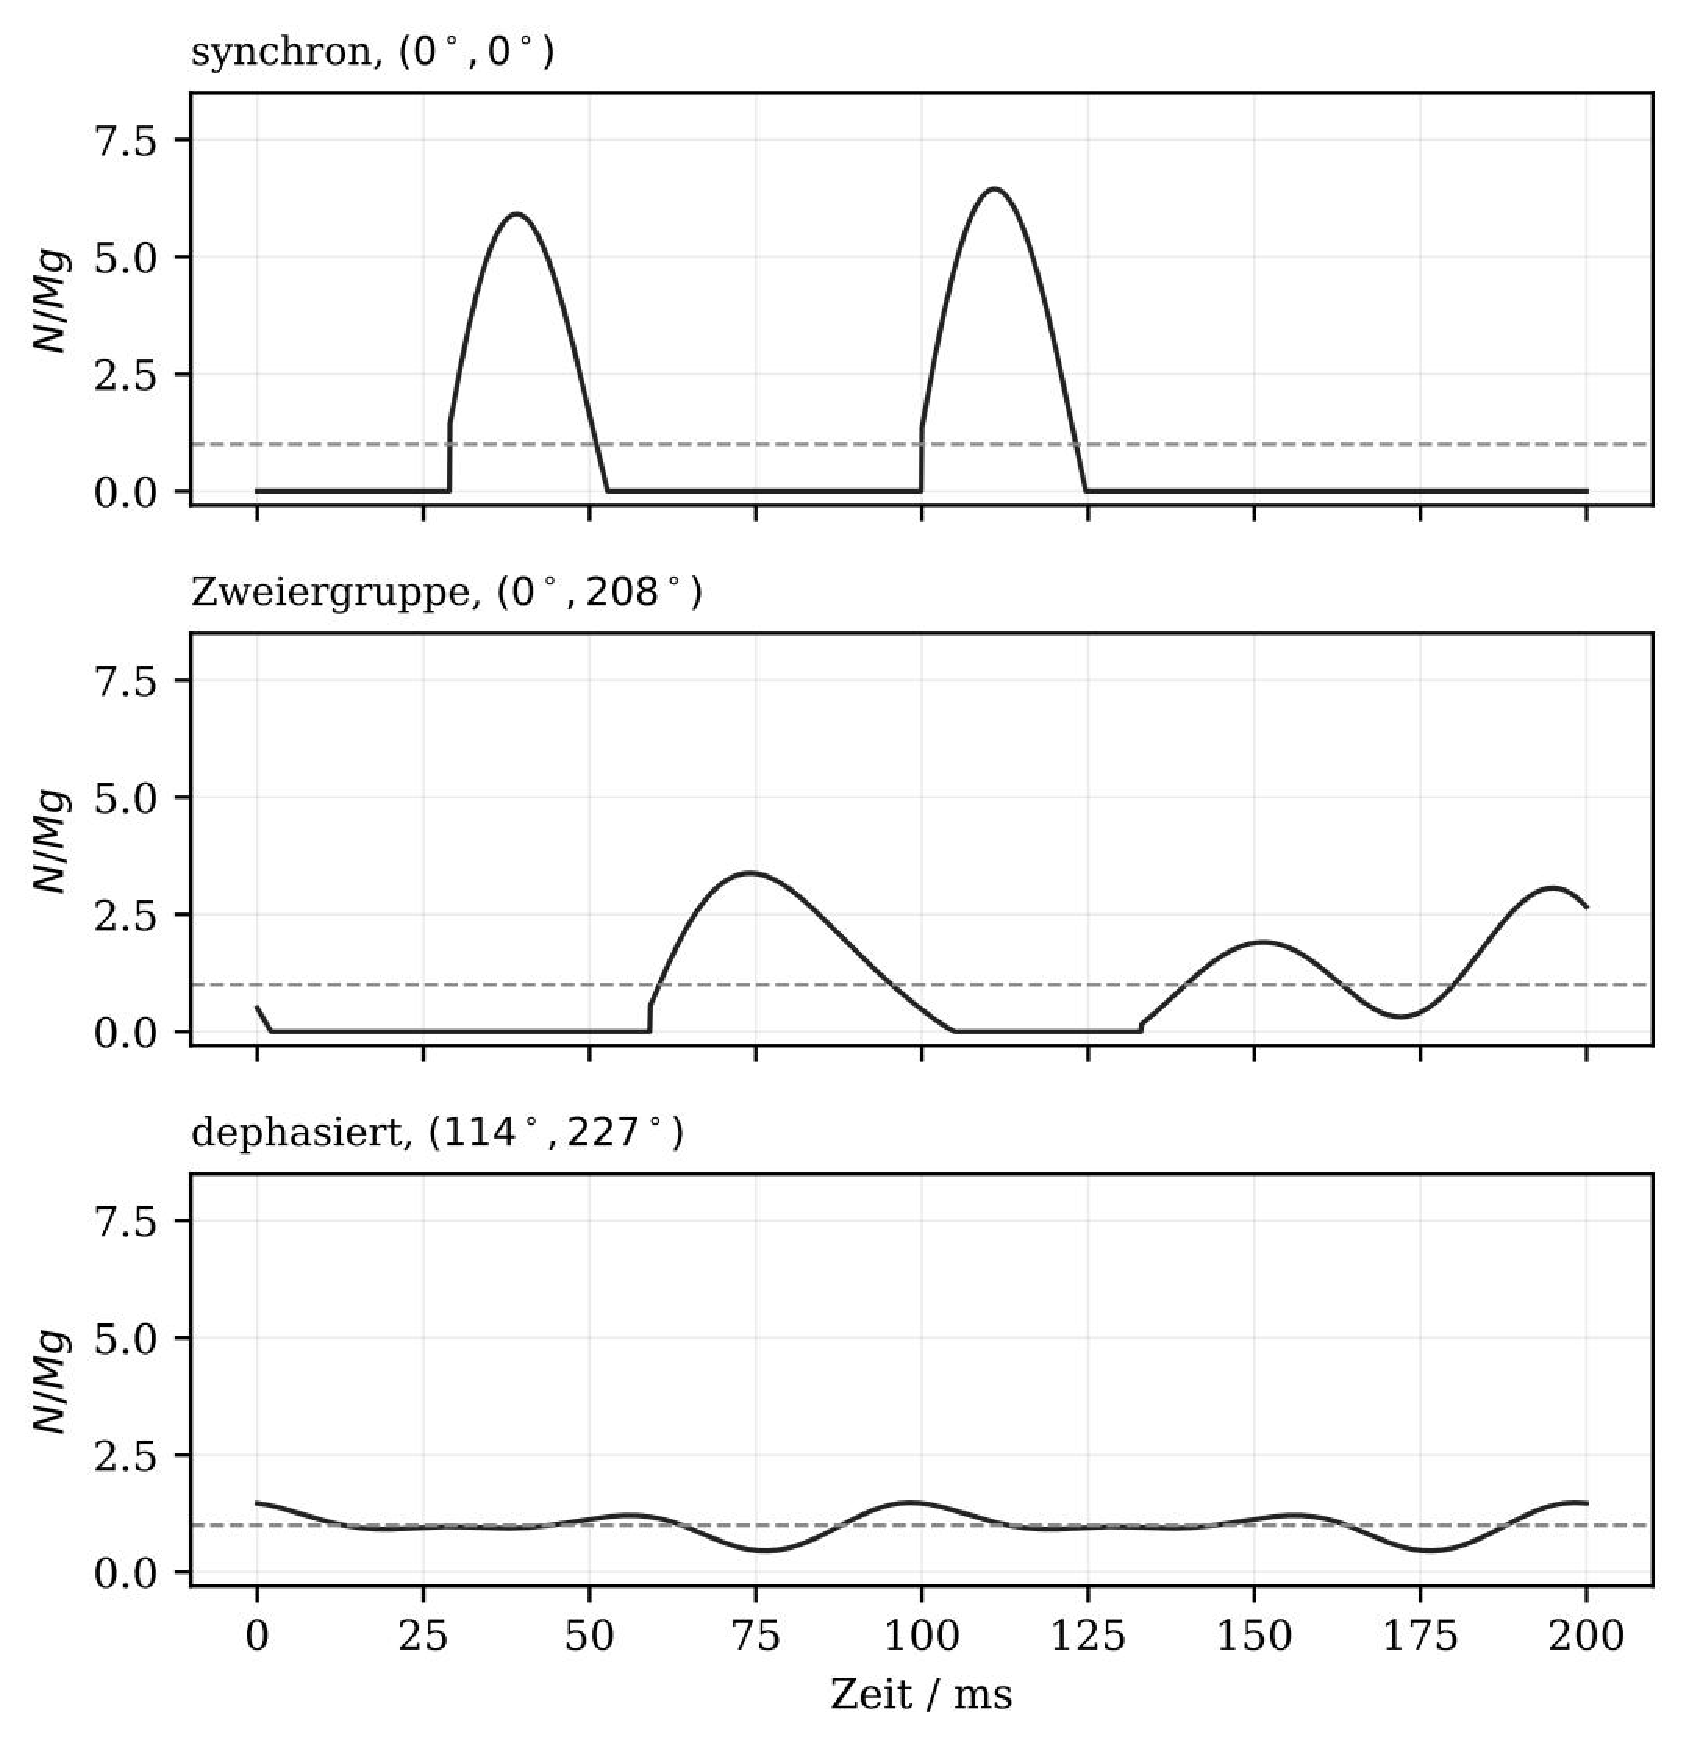
\includegraphics[width=0.78\textwidth]{Plots/zeitverlauf_regime.pdf}
  \caption{Simulierter Kraftverlauf über zwei Anregungsperioden für drei
  Regime, normiert auf die Basislinie. Gestrichelt: $N = Mg$. Oben und
  Mitte heben ab, unten bleibt der Kontakt erhalten.}
  \label{fig:zeitverlauf}
\end{figure}

Abbildung~\ref{fig:zeitverlauf} zeigt die zugehörigen Verläufe. Die
Flanke ist mit $7$ bis $8\,\mathrm{ms}$ nicht steil; sie wird durch die
Kontakteigenfrequenz $f_n \approx 19{,}7\,\mathrm{Hz}$ des weichen
Kontakts bestimmt. 99 Prozent der Wechselleistung liegen in allen vier
Regimen unterhalb von $65\,\mathrm{Hz}$, also unterhalb von etwa
$3{,}3\,f_n$.

\paragraph{Ableitung der Anforderungen.}
Damit die Flanke unverzerrt und der Liftoff-Anteil auf ein Prozent der
Periode genau erfasst wird, gelten die folgenden Regeln. Sie sind
parametrisch in $f_n$ formuliert, weil ein steiferer Kontakt --- ein
Metallpad statt Elastomer, eine härtere Feder --- $f_n$ und damit alle
Anforderungen proportional anhebt.

\begin{itemize}
\item Bandbreite der Messkette, $-3\,\mathrm{dB}$:
      $B \geq 3\,f_{99} \approx 10\,f_n$. Für die Simulationswerte
      $B \gtrsim 200\,\mathrm{Hz}$.
\item Abtastrate: $f_s \geq 10\,B$, damit die Flanke mit mindestens zehn
      Stützstellen abgebildet und die Kontaktschwelle $N_{\mathrm{thr}}$
      ohne Interpolation angewandt werden kann. Für die Simulationswerte
      $f_s \gtrsim 2\,\mathrm{kHz}$.
\item Auflösung des Liftoff-Anteils: Ein Prozent der Periode entspricht
      bei $10\,\mathrm{Hz}$ einer Millisekunde, also $f_s \geq 1\,\mathrm{kHz}$
      unabhängig von $f_n$.
\item Antialiasing-Filterung vor der Wandlung, Grenzfrequenz zwischen
      $B$ und $f_s/2$.
\end{itemize}

\paragraph{Folgen für die Wandlerauswahl.}
Ein Wägezellenwandler mit $80$ Abtastungen je Sekunde, wie er in
kostengünstigen Waagen verbreitet ist, scheidet aus: Er liefert acht
Stützstellen je Periode und zwei je Kontaktphase, seine Nyquist-Frequenz
von $40\,\mathrm{Hz}$ liegt unterhalb von $f_{99}$, und der
Liftoff-Anteil wäre auf zwölf Prozent der Periode quantisiert. Ein
24-Bit-Wandler mit programmierbarem Vorverstärker und Abtastraten bis
$30\,\mathrm{kSPS}$, wie in der Laborvariante vorgesehen, erfüllt die
Anforderungen mit einem Faktor zehn Reserve. Die Reserve ist nicht
überflüssig: Sie deckt den Fall eines steiferen Kontakts ab, ohne dass
der Wandler getauscht werden muss.

\section{Rauscheigenschaften}

Das gemessene Signal enthält thermisches Rauschen aus Sensor und
Elektronik, elektronisches Rauschen aus Verstärker und Wandler sowie
mechanisches Rauschen aus Erschütterungen und Strukturkopplung. Es wird
als stochastisch angenommen und über Varianz und spektrale Eigenschaften
charakterisiert.

Für die Wellenformfunktionale zählt weniger das Rauschen je Abtastwert
als sein Einfluss auf die Kontaktschwelle: Rauschen um $N_{\mathrm{thr}}$
herum lässt Abtastwerte zwischen Kontakt und Kontaktverlust springen und
verzerrt $\lambda$ und $N_{\min}$. Die Schwelle ist deshalb auf das
gemessene Rauschniveau zu legen, nicht auf null, und die Empfindlichkeit
gegenüber ihrer Wahl ist Teil der Robustheitsprüfungen.

\section{Drift und Stabilität}

Drift ist eine langsame Änderung des Messsignals, die nicht unmittelbar
an die Systemanregung gebunden ist. Wesentliche Quellen sind
Temperaturänderungen, Alterung des Aufnehmers, mechanische Relaxation
und Offsetdrift der Elektronik. Sie wird durch Kontrolle der
Umgebungsbedingungen gering gehalten und in der Messgleichung
ausdrücklich modelliert.

Drift verschiebt das Zeitmittel und wird deshalb von der Kontrollgröße
erfasst; die Wellenformfunktionale sind gegen einen langsamen Offset
weitgehend unempfindlich, mit der in
Abschnitt~\ref{sec:baseline-and-observables} benannten Ausnahme der
Kontaktschwelle.

\section{Messauflösung und Nachweisgrenze}

Die wirksame Auflösung des Messsystems wird durch Aufnehmerauflösung und
Rauschpegel bestimmt,
$\delta F_{\text{eff}} \approx \sqrt{\delta F_{\text{sensor}}^2 + \sigma_{\text{noise}}^2}$.

$\delta F_{\text{eff}}$ ist eine Eigenschaft der Messkette und wird aus
deren Kenngrößen bestimmt. Sie ist nicht mit der Entscheidungsschwelle
$\varepsilon_{\mathrm{phys}}$ nach Abschnitt~\ref{sec:threshold} zu
verwechseln:

\begin{itemize}
\item $\delta F_{\text{eff}}$ gibt an, welche Kraftdifferenz die
      Messkette im Einzelwert auflöst. Sie folgt aus Aufnehmerauflösung
      und Rauschpegel und lässt sich vorab aus Datenblattangaben
      abschätzen.
\item $\varepsilon_{\mathrm{phys}}$ gibt an, welche Differenz eines
      Wellenformfunktionals zwischen zwei Konfigurationen als Befund
      gelten darf. Sie folgt aus der Streuung zwischen Wiederholungen in
      einer festen Referenzkonfiguration und lässt sich nicht
      abschätzen, sondern nur messen.
\end{itemize}

Die zweite Größe ist regelmäßig deutlich größer als die erste, da sie
neben dem Rauschen auch Aufsetzen, thermischen Zustand und
Reproduzierbarkeit der Antriebe enthält. Eine Auslegung, die
$\delta F_{\text{eff}}$ als Nachweisgrenze führt, unterschätzt daher die
tatsächlich erforderliche Auflösung.

\section{Hilfskanäle}

Zwei Hilfskanäle werden synchron zum Kraftsignal aufgezeichnet.

Ein \textbf{Beschleunigungsaufnehmer am Gehäuse} liefert eine
unabhängige Prüfung des Liftoffs: Während der Kontakt abgehoben ist,
befindet sich das Gehäuse im freien Fall und der Aufnehmer zeigt
näherungsweise null. Der so bestimmte Liftoff-Anteil muss mit dem aus
dem Kraftsignal übereinstimmen; eine Abweichung weist auf eine falsch
gesetzte Kontaktschwelle oder auf ein Problem der Kraftmesskette hin.
Zugleich verifiziert der Aufnehmer die innere Bewegung.

Ein \textbf{Synchronkanal} zeichnet das Phasen- und Antriebssignal der
Steuerung mit. Er ermöglicht phasenstarre Mittelung, Kreuzkorrelation
und die Prüfung, ob ein Signalanteil mit dem Antriebstakt korreliert
statt mit dem mechanischen Zustand --- die Signatur der
elektromagnetischen Einkopplung nach Kapitel~\ref{chap:artefakt}.

Beide Kanäle gelten nicht als primäre Observablen, sondern als
Kontextinformation für Synchronisation, Artefaktanalyse und
Laufvalidierung.

\section{Kontrolle der Umgebungsbedingungen}

Temperatur, Erschütterungen, Luftströmungen und elektromagnetische
Störeinflüsse werden kontrolliert oder überwacht. Wo eine vollständige
Kontrolle nicht möglich ist, werden die Umgebungsgrößen aufgezeichnet
und in die Auswertung einbezogen. Netzbrumm bei $50\,\mathrm{Hz}$ liegt
innerhalb des geforderten Frequenzbereichs und kann nicht weggefiltert
werden, ohne die Flanke zu beschädigen; er ist durch Schirmung und
getrennte Versorgung zu vermeiden und im Leerlauf nachzuweisen.

\section{Messunsicherheit}

Die gesamte Messunsicherheit setzt sich zusammen aus Rauschen, Drift
und Kalibrierunsicherheit,
$\sigma_{\text{total}}^2 = \sigma_{\text{noise}}^2 + \sigma_{\text{drift}}^2 + \sigma_{\text{cal}}^2$.
Die Fortpflanzung erfolgt durchgängig in der gesamten Auswertung. Für die
Wellenformfunktionale tritt die Unsicherheit der Kontaktschwelle als
eigener Beitrag hinzu.

\section{Zusammenfassung}

Das Messsystem wird ausdrücklich als Teil des experimentellen Rahmens
modelliert. Seine Auslegung folgt aus der Simulation: Nennlast am
Spitzenwert, Bandbreite an der Kontakteigenfrequenz, Abtastrate an der
Flanke und am Liftoff-Anteil. Die statische Kalibrierung sichert die
Kennlinie um den Arbeitspunkt; ihre Gültigkeit über den gesamten
Kraftbereich und unter intermittierendem Kontakt bleibt die offene
Frage der Messkette.

% ------------------------------------------------------

\chapter{Versuchsprotokoll und Datenerfassung}
\label{chap:protokoll}

\section{Überblick}

Das Versuchsprotokoll soll sicherstellen, dass Messungen unter
verschiedenen Systemzuständen vergleichbar, reproduzierbar und innerhalb
des in den vorangehenden Kapiteln festgelegten Rahmens auslegbar sind. Da
die Zielgrößen Funktionale der Kontaktkraft-Wellenform sind und die
Kontrollgröße einen erhaltungsgarantierten Sollwert besitzt, muss das
Protokoll unkontrollierte Variation gering halten und alle maßgeblichen
Schritte vor der Auslegung der Daten festlegen.

Das experimentelle Vorgehen verbindet daher gesteuerte
Zustandsübergänge, synchronisierte Signalerfassung, wiederholte Messungen
und vorab festgelegte Auswerteregeln.

\section{Messziel}

Das Protokoll bedient die beiden Spuren nach
Kapitel~\ref{chap:statistik} und liefert je Lauf zwei Arten von Größen.

Für die Spur der Apparaturqualifikation ist dies die Kontrollgröße

\begin{equation}
\Delta \bar{F}_{\text{Zustand}} = \bar{F}_{A} - \bar{F}_{B},
\end{equation}

deren wahrer Wert nach Gleichung~\eqref{eq:baseline-ch3} null ist. Das
Protokoll erzeugt sie nicht, um einen Effekt zu finden, sondern um zu
prüfen, ob die Kette einen bekannten Nullwert als null wiedergewinnt.

Für die Spur der Zielgrößen sind dies die Wellenformfunktionale
$\gamma_1$, $\lambda$, $A$ und $N_{\min}$ nach
Abschnitt~\ref{sec:target-quantities}, berechnet je Erfassungsfenster.

Beide Größenarten werden auf denselben Fenstern gebildet und im selben
Lauf erhoben. Sie werden getrennt ausgewertet und nie zusammengeführt.

\section{Definition eines Messlaufs}

Ein einzelner Messlauf besteht aus den folgenden Stufen:

\begin{enumerate}
\item Initialisierung von System und Messkette,
\item Stabilisierung des Aufbaus unter kontrollierten Randbedingungen,
\item Ausführung des Zustands $A$ und Erfassung des zugehörigen
      Kraftsignals,
\item gesteuerter Übergang zum Zustand $B$,
\item Ausführung des Zustands $B$ und Erfassung des zugehörigen
      Kraftsignals,
\item Beendigung und Sicherung aller aufgezeichneten Daten und
      Metadaten.
\end{enumerate}

Ein Lauf gilt nur dann als gültig, wenn während der Ausführung kein
vorab festgelegtes Ausschlusskriterium verletzt wurde.

\section{Initialisierung}

Vor jedem Messlauf werden die folgenden Schritte durchgeführt:

\begin{itemize}
\item Prüfung der mechanischen Einspannung und der Sensoranbindung,
\item Initialisierung des Datenerfassungssystems,
\item Prüfung der Sensor-Nulllage und der Signalverfügbarkeit,
\item Aktivierung der Umgebungsüberwachung,
\item Festlegung der Aktuierungsparameter für den bevorstehenden Lauf.
\end{itemize}

Bei Bedarf wird nach dem Start eine Beruhigungszeit eingelegt, damit
Einschwingvorgänge aus Aktivierung, thermischer Angleichung oder
mechanischer Relaxation vor Beginn der Datenerfassung abklingen.

\section{Definition der Versuchszustände}

Die Versuchszustände $A$ und $B$ werden operativ über verschiedene Sätze
innerer Steuerparameter definiert. Diese können sich in
Phasenkonfiguration, Zeitverlauf oder innerem Anregungsmuster
unterscheiden, während die äußeren Randbedingungen unverändert bleiben.

Zweck der Zustandsdefinition ist nicht die Kodierung einer theoretischen
Auslegung, sondern die Festlegung zweier reproduzierbarer
Betriebsbedingungen, deren gemessene Ausgangsgrößen statistisch
verglichen werden können.

Zur Sicherung der Vergleichbarkeit werden alle Parameter, die nicht
ausdrücklich zur Definition des Zustandswechsels dienen, innerhalb eines
Versuchs festgehalten.

\section{Zustandsfolge und Zeitablauf}

Innerhalb jedes Laufs sind Reihenfolge und Dauer der Messabschnitte
vorab festgelegt. Jeder Zustand wird hinreichend lange gehalten, damit
ein statistisch belastbarer Signalabschnitt erfasst werden kann.

Eine typische Folge kann bestehen aus:

\begin{enumerate}
\item einem Basisabschnitt vor der Aktuierung,
\item einem Stabilisierungsintervall nach Eintritt in den Zustand $A$,
\item dem Erfassungsfenster für den Zustand $A$,
\item einem gesteuerten Übergangsintervall,
\item einem Stabilisierungsintervall nach Eintritt in den Zustand $B$,
\item dem Erfassungsfenster für den Zustand $B$,
\item einem wahlweisen Basisabschnitt nach dem Lauf.
\end{enumerate}

Die Stabilisierungsintervalle verringern die Verunreinigung durch
Einschwingvorgänge unmittelbar nach einem Zustandswechsel.

\section{Datenerfassung}

Das gemessene Kraftsignal wird als Zeitreihe

\begin{equation}
F_{\text{meas}}(t)
\end{equation}

mit einem synchronisierten Datenerfassungssystem aufgezeichnet. Neben dem
primären Kraftsignal können Hilfskanäle aufgezeichnet werden, darunter:

\begin{itemize}
\item Taktsignale der Aktuierung,
\item Phasenreferenzen,
\item Temperaturdaten,
\item Erschütterungs- oder Beschleunigungssignale,
\item Statusmerkmale des Systems.
\end{itemize}

Diese Hilfssignale gelten nicht als primäre Observablen des
Hypothesentests, sondern als Kontextinformation für Synchronisation,
Artefaktanalyse und Laufvalidierung.

\section{Abtaststrategie}
\label{sec:abtaststrategie}

Die Abtastrate wird so gewählt, dass sowohl dynamische Änderungen als
auch statistische Eigenschaften des gemessenen Signals hinreichend
aufgelöst werden. Die Wahl der Abtastfrequenz muss zwei Bedingungen
erfüllen:

\begin{itemize}
\item die maßgeblichen zeitlichen Änderungen des Signals werden ohne
      Aliasing erfasst,
\item innerhalb jedes Erfassungsfensters stehen genügend Datenpunkte zur
      verlässlichen Schätzung von Mittelwert und Varianz zur Verfügung.
\end{itemize}

Bei Bedarf kann überabgetastet und in der Nachverarbeitung kontrolliert
zusammengefasst oder gefiltert werden. Die konkreten Anforderungen ---
Bandbreite $B \geq 10\,f_n$, Abtastrate $f_s \geq 10\,B$, mindestens
$1\,\mathrm{kHz}$ --- sind in Abschnitt~\ref{sec:bandbreite} aus der
Kontaktflanke abgeleitet.

\paragraph{Fensterlänge und Konvergenz.}
Je Phasenkonfiguration werden mindestens $100$ Anregungszyklen
ausgewertet. Diese Zahl ist eine Untergrenze, keine Vorgabe: Nach
Abschnitt~\ref{sec:track1-sim} trägt das Fenstermittel der Kontrollgröße
einen Randterm $\delta_w = \Delta v_S/(g\,T_w)$, der bei aperiodischer
Bewegung nur mit $T_w^{-1}$ fällt; ein Fenster von $100$ Zyklen lässt dort
noch Residuen im Promillebereich. Die
erforderliche Fensterlänge wird deshalb nicht angenommen, sondern
nachgewiesen: Für die intermittenteste Konfiguration der Kampagne wird
die Auswertung mit verdoppeltem Fenster wiederholt, und die Fensterlänge
gilt erst dann als ausreichend, wenn die Kontrollgröße dabei um weniger
als $\varepsilon_{\mathrm{phys}}$ wandert. Das Fenster umfasst in jedem Fall eine ganze Zahl von Anregungsperioden
und wird erst nach abgeschlossenem Einschwingen geöffnet. Für den
Randterm gilt die Schranke $|\delta_w| \le 2\,v_{S,\max}/(g\,T_w)$ nach
Gleichung~\eqref{eq:randterm}.

\section{Aufgezeichnete Metadaten}

Für jeden Lauf werden die folgenden Metadaten dokumentiert:

\begin{itemize}
\item Datum und Uhrzeit des Versuchs,
\item Kennung des Laufs,
\item Parametersatz zur Definition der Zustände $A$ und $B$,
\item Dauer aller Erfassungsfenster,
\item Umgebungsbedingungen,
\item Sensorkonfiguration und Kalibrierstatus,
\item Vermerke zu Auffälligkeiten oder Unterbrechungen.
\end{itemize}

Die Aufzeichnung der Metadaten sichert die Nachvollziehbarkeit und trägt
die spätere Artefaktanalyse.

\section{Messlogik}

Die Logik des Versuchs folgt einem messzentrierten Vorgehen. Die
Leitfrage ist, ob das gemessene Signal einen reproduzierbaren Unterschied
im mittleren Verhalten zwischen den Zuständen $A$ und $B$ aufweist.

Jeder Messlauf liefert entsprechend zwei Signalabschnitte, die den beiden
Zuständen zugeordnet sind. Für jeden Abschnitt werden statistische
Kennwerte berechnet, mindestens:

\begin{itemize}
\item Mittelwert,
\item Standardabweichung,
\item Abschnittsdauer,
\item Anzahl der Abtastwerte.
\end{itemize}

Der wesentliche Schätzwert je Lauf ergibt sich dann als Differenz der
Abschnittsmittelwerte,

\begin{equation}
\Delta \bar{F}^{(i)}_{\text{Zustand}} = \bar{F}^{(i)}_{A} - \bar{F}^{(i)}_{B},
\end{equation}

wobei der hochgestellte Index $(i)$ den $i$-ten Lauf bezeichnet.

Über wiederholte Läufe hinweg wird die Verteilung von
$\Delta \bar{F}^{(i)}_{\text{Zustand}}$ statistisch ausgewertet.

\section{Wiederholte Messungen}

Ein einzelner Lauf trägt keinen belastbaren Schluss. Der Versuch wird
daher unter nominell identischen Bedingungen mehrfach wiederholt.

Wiederholte Läufe dienen mehreren Zwecken:

\begin{itemize}
\item der Schätzung der Streuung zwischen Läufen,
\item der Beurteilung der Reproduzierbarkeit,
\item der Verringerung der zufälligen Unsicherheit,
\item dem Erkennen instabilen oder nichtstationären Verhaltens.
\end{itemize}

Die Zahl der Wiederholungen richtet sich nach dem erwarteten
Signal-Rausch-Verhältnis und der geforderten statistischen Sicherheit.

\section{Ausschluss- und Gültigkeitskriterien}

Um nachträgliche Auswahlverzerrung zu vermeiden, werden die
Gültigkeitskriterien für Läufe vor der Datenauswertung festgelegt. Ein
Lauf kann beispielsweise ausgeschlossen werden, wenn

\begin{itemize}
\item das Datenerfassungssystem ausfällt oder die Synchronisation
      verliert,
\item das Sensorsignal in die Sättigung geht,
\item eine vorab festgelegte Umgebungsschwelle überschritten wird,
\item die Aktuierungsfolge von der vorgegebenen Zustandsdefinition
      abweicht,
\item starke Störungen oder Unterbrechungen während des
      Erfassungsfensters auftreten.
\end{itemize}

Alle Ausschlüsse sind zu dokumentieren und ausdrücklich zu begründen.

\section{Behandlung von Drift und Einschwingvorgängen}

Die Abgrenzung der Zielgröße gegen Drift und Einschwingvorgänge
erfordert besondere Sorgfalt. Deshalb gilt:

\begin{itemize}
\item nach Zustandswechseln werden Stabilisierungsfenster eingelegt,
\item vor und nach der Hauptmessung können Basisabschnitte aufgezeichnet
      werden,
\item Langzeittrends über die Läufe hinweg werden überwacht,
\item Zustandsvergleiche erfolgen innerhalb einer kontrollierten
      zeitlichen Struktur.
\end{itemize}

Es wird nicht angenommen, dass Drift verschwindet; das Protokoll soll
vielmehr das Risiko verringern, dass Drift als zustandsabhängige
Mittelwertverschiebung fehlgedeutet wird.

\section{Datenaufbereitung}

Vor der formalen statistischen Auswertung können die Rohdaten begrenzte
Vorverarbeitungsschritte durchlaufen, sofern diese einheitlich definiert
und auf alle Läufe gleich angewandt werden. Dazu können gehören:

\begin{itemize}
\item die Synchronisation der Signalkanäle,
\item die Segmentierung in Basis-, Übergangs- und Zustandsfenster,
\item das Entfernen ungültiger Abtastwerte aus Erfassungsfehlern,
\item eine wahlweise Filterung, begründet durch die
      Sensoreigenschaften.
\end{itemize}

Jede Vorverarbeitung muss die Auslegbarkeit der gemessenen Mittelwerte
erhalten und darf keine zustandsabhängige Verzerrung einbringen.

\section{Anschluss an die statistische Auswertung}

Ergebnis des Messprotokolls ist ein strukturierter Datensatz aus
wiederholten Schätzwerten von $\Delta \bar{F}_{\text{Zustand}}$, den
zugehörigen Varianzen und den Metadaten der Läufe.

Diese Ausgaben bilden die Grundlage des statistischen
Entscheidungsrahmens im folgenden Kapitel. Das Protokoll selbst
entscheidet nicht über die Ablehnung der Nullhypothese; es stellt
sicher, dass die aufgezeichneten Daten für einen gültigen statistischen
Test geeignet sind.

\section{Zwischenfazit}

Das Versuchsprotokoll legt ein kontrolliertes Vorgehen zum Vergleich
zweier Systemzustände anhand gemessener Kraftsignale fest. Seine
zentralen Elemente sind vorab festgelegte Zustandsdefinitionen,
synchronisierte Datenerfassung, wiederholte Läufe und ausdrückliche
Gültigkeitskriterien.

Diese Struktur soll sicherstellen, dass jeder beobachtete Unterschied
zwischen den Zuständen $A$ und $B$ innerhalb eines durchsichtigen und
falsifizierbaren Messrahmens bewertet werden kann.

\section{Systematische Artefaktanalyse}

\begin{table}[htbp]
\centering
\caption{Systematische Artefaktanalyse für Messungen
zustandsabhängiger Mittelwertverschiebungen.}
\small
\begin{tabular}{@{}>{\raggedright\arraybackslash}p{2.6cm} >{\raggedright\arraybackslash}p{3.8cm} >{\raggedright\arraybackslash}p{3.8cm} >{\raggedright\arraybackslash}p{4.5cm}@{}}
\toprule
Artefakt & Physikalischer Mechanismus & Erwartete Signalsignatur & Gegenmaßnahme / Prüfstrategie \\
\midrule

Thermische Drift
& Temperaturabhängige Ausdehnung mechanischer Bauteile oder Offsetdrift des Sensors
& Langsame monotone oder niederfrequente Änderung, unabhängig vom Anregungszustand
& Temperaturüberwachung, Abzug der Basislinie, Nullversuche ohne Anregung \\

Mechanisches Spiel und Lose
& Nichtlineare Kontakteffekte, Spalte, Hysterese in bewegten Teilen
& Zustandsabhängige Asymmetrie, gegebenenfalls Hystereseschleifen im Kraftsignal
& Versuche mit beidseitiger Anregung, Prüfung der Umkehrsymmetrie \\

Offsetdrift des Sensors
& Elektronische Drift im Messsystem, Analog-Digital-Wandler und Verstärker
& Über die Zeit gleichmäßige Verschiebung, alle Zustände gleichermaßen betreffend
& Kalibrierung vor und nach den Läufen, Referenzmessungen \\

Elektro\-magnetische Kopplung
& Von Aktoren induzierte Ströme, die auf die Sensorelektronik wirken
& Korrelation mit dem Aktuierungstakt statt mit dem mechanischen Zustand
& Schirmung, getrennte Spannungsversorgung, Kontrollversuche \\

Schwingungs\-kopplung
& Äußere oder innere Schwingungen, die in die Messachse einkoppeln
& Oszillatorische Signalanteile, frequenzkorreliert mit Systemmoden
& Frequenzanalyse, entkoppelnde Lagerung, Kontrollläufe \\

Verzerrung durch Datenverarbeitung
& Artefakte aus Filterung, Fensterung oder Mittelung
& Künstliche Glättung oder systematische Verzerrung der Mittelwertschätzung
& Vergleich von Roh- und verarbeiteten Daten, Validierung der Algorithmen \\

Abtast- und Synchronisationsfehler
& Versatz zwischen Anregungs- und Messzeitbasis
& Phasenabhängige Verzerrungen oder künstliche Mittelwertverschiebungen
& Prüfung der Zeitsynchronisation, hochauflösende Zeitstempel \\

\bottomrule
\end{tabular}
\end{table}

\clearpage

\subsection{Artefaktunterscheidung und Signalzuordnung}

Der Nachweis einer echten zustandsabhängigen Mittelwertverschiebung
erfordert eine klare Abgrenzung gegen mögliche Artefaktbeiträge. Jeder
maßgeblichen Artefaktklasse ist eine kennzeichnende Signalsignatur
zugeordnet, die sich systematisch mit dem beobachteten Messverhalten
vergleichen lässt.

Der experimentelle Rahmen ist daher so angelegt, dass eine Unterscheidung
dieser Signaturen anhand ihrer strukturellen Eigenschaften möglich ist.

\vspace{0.5em}

\textbf{Grundsätze der Artefaktunterscheidung:}

\begin{itemize}
    \item \textbf{Zeitabhängigkeit:}
    Driftbedingte Effekte zeigen typischerweise langsame, monotone oder
    niederfrequente Änderungen, die nicht unmittelbar an den
    Systemzustand gekoppelt sind.

    \item \textbf{Zustandskorrelation:}
    Ein echter Effekt muss mit dem gesteuerten Systemzustand korrelieren
    und nicht mit äußeren oder unkontrollierten Größen.

    \item \textbf{Symmetrieverhalten:}
    Mechanische Nichtlinearitäten wie Lose oder Hysterese führen häufig
    zu asymmetrischen oder richtungsabhängigen Signalmustern, die sich
    durch Umkehrversuche prüfen lassen.

    \item \textbf{Frequenzmerkmale:}
    Schwingungs- oder elektromagnetische Artefakte sind typischerweise
    an bestimmte Frequenzanteile gebunden und lassen sich durch
    Spektralanalyse erkennen.

    \item \textbf{Systemunabhängigkeit:}
    Artefakte aus der Messkette, etwa Sensordrift, betreffen alle
    Zustände gleichermaßen und lassen sich durch Referenzmessungen
    isolieren.
\end{itemize}

\vspace{0.5em}

\textbf{Zuordnung zum gemessenen Signal:}

Eine echte zustandsabhängige Mittelwertverschiebung ist durch die
folgenden Kriterien bestimmt:

\begin{itemize}
    \item Übereinstimmung über unabhängige Versuchsläufe hinweg
    \item Reproduzierbare Abhängigkeit vom Systemzustand
    \item Stabilität unter Variation der Versuchsparameter
    \item Fehlende Korrelation mit bekannten Artefaktsignaturen
\end{itemize}

\vspace{0.5em}

Artefaktbedingte Signale verletzen demgegenüber typischerweise
mindestens eine dieser Bedingungen. Die gemeinsame Anwendung der
genannten Kriterien erlaubt eine strukturierte Klassifikation
beobachteter Signalanteile und trägt die Trennung echter Effekte von
Messartefakten.

\vspace{0.5em}

Dieses Vorgehen setzt die Existenz eines physikalischen Effekts nicht
voraus. Es liefert vielmehr einen systematischen Rahmen zur Falsifikation,
indem geprüft wird, ob sich das beobachtete Signalverhalten vollständig
durch bekannte Artefaktmechanismen erklären lässt.

\begin{quote}
Ein Signal wird nur dann als Kandidat für eine echte zustandsabhängige
Mittelwertverschiebung eingestuft, wenn es sämtliche definierten
Kriterien gleichzeitig erfüllt. Wird ein einziges Kriterium verfehlt,
erfolgt die Einstufung als möglicher Artefaktbeitrag.
\end{quote}

\subsection{Statistische Anforderungen an das Protokoll}

Der statistische Entscheidungsrahmen selbst steht in
Kapitel~\ref{chap:statistik}. Der vorliegende Unterabschnitt legt fest,
was das Protokoll liefern muss, damit dieser Rahmen überhaupt anwendbar
ist. Die Trennung ist bewusst: Das Protokoll entscheidet nichts, es
erzeugt die Voraussetzungen einer Entscheidung.

\vspace{0.5em}

\textbf{Was je Lauf entstehen muss.}

Ein gültiger Lauf liefert einen Datensatz aus:

\begin{itemize}
    \item den beiden Fenstermittelwerten $\bar{F}_{A}^{(i)}$ und
    $\bar{F}_{B}^{(i)}$ nach den Gleichungen~\eqref{eq:fenster-a}
    und~\eqref{eq:fenster-b}, aus denen die Kontrollgröße gebildet wird,
    \item den vier Zielfunktionalen je Fenster,
    \item der Fensterlänge in ganzen Anregungsperioden sowie der Zahl der
    Abtastwerte je Fenster,
    \item den Hilfskanälen und Umgebungsgrößen des Laufs,
    \item dem Prüfergebnis gegen die Gültigkeitskriterien.
\end{itemize}

Fehlt eine dieser Angaben, ist der Lauf für die Auswertung nicht
verwendbar. Das gilt insbesondere für die Fensterlänge in ganzen
Perioden: Bei angeschnittenem Zyklus sind Schiefe und Liftoff-Anteil
verzerrt, ohne dass dies im Ergebnis sichtbar würde.

\vspace{0.5em}

\textbf{Was vor der ersten Messung festzulegen ist.}

Die folgenden Größen werden vor Beginn der Datenerhebung festgeschrieben
und danach nicht mehr verändert:

\begin{itemize}
    \item das Signifikanzniveau $\alpha$ und das Verfahren zur
    Berücksichtigung der Multiplizität,
    \item die Zahl der Läufe $N$, abgeleitet aus
    $\hat{\sigma}_{\mathrm{ref}}$ der Wiederholmesskampagne,
    \item die Zahl der Bootstrap-Resamples,
    \item die operative Kontaktschwelle $N_{\mathrm{thr}}$ aus
    Gleichung~\eqref{eq:liftoff},
    \item die Schwellen $\varepsilon_{\mathrm{phys}}$,
    $\varepsilon_{\perp}$ und $\varepsilon_{\mathrm{ctrl}}$,
    \item die Ausschluss- und Gültigkeitskriterien für Läufe.
\end{itemize}

Die Reihenfolge ist zwingend: Die Wiederholmesskampagne in der
Referenzkonfiguration $S_{\mathrm{ref}}$ geht dem Phasensweep voraus,
weil $\hat{\sigma}_{\mathrm{ref}}$ sowohl die Schwellen als auch die
erforderliche Laufzahl bestimmt. Eine nachträgliche Festlegung dieser
Werte aus den Sweep-Daten selbst wäre zirkulär.

\vspace{0.5em}

\textbf{Anforderungen an die Messreihenfolge.}

\begin{itemize}
    \item Die Reihenfolge der Phasenkonfigurationen wird randomisiert.
    Ein monotoner Sweep verläuft parallel zur thermischen Drift der
    Apparatur und erzeugt eine scheinbare Phasenabhängigkeit, die von
    einer echten nicht zu unterscheiden ist.
    \item Die Referenzkonfiguration wird in den Sweep eingestreut, nicht
    nur an dessen Anfang und Ende gemessen. Nur so lässt sich eine
    Veränderung der Wiederholpräzision im Verlauf der Kampagne erkennen.
    \item Zustandspaare $A$ und $B$ werden innerhalb eines Laufs erhoben
    und nicht über Läufe hinweg gebildet, damit eine zeitgebundene
    Verschiebung beide Fenster gleichermaßen trifft.
    \item Der Sweep wird zweistufig gefahren: zunächst ein grobes Raster
    über der gesamten Phasenebene, dann eine Verfeinerung an den
    Regimegrenzen und um die triphasische Konfiguration. Die Verfeinerung
    wird vor der Grobmessung als Regel festgelegt, nicht nach Sichtung
    der Daten als Auswahl.
\end{itemize}

\vspace{0.5em}

\textbf{Pflichtläufe vor dem Sweep.}

\begin{itemize}
    \item Der \textbf{Leerlauf mit bestromter, aber blockierter
    Aktuierung}, nach Abschnitt~\ref{sec:kontrollgrenze} der
    wichtigste Einzelversuch der Kampagne. Er wird vor dem Sweep und
    nach jedem Umbau wiederholt.
    \item Die \textbf{Wiederholmesskampagne} in $S_{\mathrm{ref}}$,
    aus der $\hat{\sigma}_{\mathrm{ref}}$ und damit
    $\varepsilon_{\mathrm{phys}}$ folgen. Sie schließt Neuaufsetzen
    des Gehäuses zwischen den Wiederholungen ein.
    \item Ein \textbf{Sinus-Referenzlauf}, falls ein sinusförmiger
    Antrieb verfügbar ist: Er liefert nach
    Abschnitt~\ref{sec:sinus-sweep} die aus Transmissibilität und Hub
    berechenbare Liftoff-Schwelle $R_c$ als zweite Prüfgröße mit
    bekannter Antwort
    und beziffert in der Messung den Beitrag der Profilasymmetrie.
\end{itemize}

\vspace{0.5em}

\textbf{Anforderungen an die Unabhängigkeit.}

Die Auswertung nach Kapitel~\ref{chap:statistik} setzt näherungsweise
unabhängige Läufe voraus. Das Protokoll trägt dieser Annahme durch
Stabilisierungszeiten, durch die Überwachung von Langzeittrends und durch
die Aufzeichnung der Laufreihenfolge Rechnung. Vollständig sichern lässt
sie sich nicht: Thermische Relaxation und Setzvorgänge in der Einspannung
wirken über Laufgrenzen hinweg. Wo die Annahme fraglich bleibt, ist dies
im Ergebnis auszuweisen und nicht durch die Wahl des Testverfahrens zu
verdecken.

\vspace{0.5em}

\textbf{Was das Protokoll ausdrücklich nicht festlegt.}

Das Protokoll trifft keine Entscheidung über Hypothesen. Insbesondere
wird die in früheren Fassungen dieser Arbeit verwendete
Go/No-Go-Klassifikation, in der die Ablehnung der Nullhypothese den
positiven Ausgang darstellte, nicht mehr angewandt. Unter
Gleichung~\eqref{eq:baseline-ch3} ist der wahre Wert der Kontrollgröße
null; eine Ablehnung der zugehörigen Nullhypothese wäre ein
Apparaturfehler und kein Befund. Die maßgebliche Klassifikation steht in
Abschnitt~\ref{sec:decision-class}.


% ------------------------------------------------------

\chapter{Statistischer Entscheidungsrahmen}
\label{chap:statistik}

\section{Überblick}

Der statistische Rahmen arbeitet auf zwei Spuren, die nacheinander
ausgewertet und nie zusammengeführt werden:

\begin{description}
  \item[Spur~1 --- Qualifikation der Apparatur.] Auswertung der
        Kontrollgröße gegen ihren bekannten Nullwert. Legt die
        Nachweisschwelle fest und begrenzt die unentdeckte systematische
        Verschiebung.
  \item[Spur~2 --- Auswertung der Zielgrößen.] Auswertung der
        Wellenformfunktionale gegen die Phasenkonfiguration unter
        Verwendung der aus Spur~1 gewonnenen Schwelle.
\end{description}

Alle Entscheidungskriterien werden vor der Auswertung festgelegt. Spur~2
wird nicht ausgewertet, wenn Spur~1 scheitert.

\section{Spur 1: Kontrollgröße}

\subsection{Schätzer}

Für $N$ Läufe sind Stichprobenmittel und Stichprobenvarianz der
Kontrollgröße

\begin{align}
  \hat{\mu}_{\Delta} &= \frac{1}{N}\sum_{i=1}^{N}
      \Delta \bar{F}^{(i)}_{\mathrm{Zustand}},
  \label{eq:mu-hat}\\[4pt]
  \hat{\sigma}^{2}_{\Delta} &= \frac{1}{N-1}\sum_{i=1}^{N}
      \Bigl( \Delta \bar{F}^{(i)}_{\mathrm{Zustand}}
             - \hat{\mu}_{\Delta} \Bigr)^{2}.
  \label{eq:sigma-hat}
\end{align}

\subsection{Spezifitätstest}

Die Prüfgröße

\begin{equation}
  T = \frac{\hat{\mu}_{\Delta}}{\hat{\sigma}_{\Delta}/\sqrt{N}}
  \label{eq:t-stat}
\end{equation}

folgt unter $H_{0}^{\mathrm{ctrl}}$ einer Student-$t$-Verteilung mit
$N-1$ Freiheitsgraden. Da der wahre Wert von $\mu_{\Delta}$ nach
Gleichung~\eqref{eq:baseline-ch3} null ist, entscheidet dieser Test keine
physikalische Frage. Er misst das Falsch-Positiv-Verhalten der
vollständigen Schlusskette gegen eine bekannte Grundwahrheit.

Die Auslegung ist gegenüber dem üblichen Hypothesentest umgekehrt, und
sie folgt einer Äquivalenzlogik, nicht einer Signifikanzlogik. Der
Grund: Das Ausbleiben eines signifikanten Ergebnisses ist kein Beleg.
Bei kleiner Laufzahl und großer Streuung ist $|T| \leq t_{\alpha/2,\,N-1}$
mühelos erfüllt und sagt über die Apparatur nichts. Qualifiziert ist die
Kette erst, wenn sie nachweislich \emph{keine} Verschiebung oberhalb
einer vorab festgelegten Toleranz trägt. Mit dem Konfidenzintervall

\begin{equation}
  \bigl[\,\hat{\mu}_{\Delta} - t_{\alpha/2,\,N-1}\,\hat{\sigma}_{\Delta}/\sqrt{N},\;
        \hat{\mu}_{\Delta} + t_{\alpha/2,\,N-1}\,\hat{\sigma}_{\Delta}/\sqrt{N}\,\bigr]
  \label{eq:ci-control}
\end{equation}

und der Toleranz $\varepsilon_{\mathrm{ctrl}}$ nach
Abschnitt~\ref{sec:threshold} gilt:

\begin{itemize}
  \item Das Intervall schließt null aus: Die Kette meldet eine
        Differenz, die nicht existieren kann. \textbf{Apparaturfehler.}
        Die Kampagne wird angehalten und der Artefaktkatalog des
        Kapitels~\ref{chap:artefakt} vor jeder weiteren Messung
        abgearbeitet.
  \item Das Intervall liegt vollständig innerhalb
        $\pm\varepsilon_{\mathrm{ctrl}}$: Die Kette trägt keine
        Verschiebung, die für die Zielgrößen erheblich wäre.
        \textbf{Qualifiziert.}
  \item Das Intervall schließt null ein, reicht aber über
        $\pm\varepsilon_{\mathrm{ctrl}}$ hinaus: Die Präzision genügt
        nicht, um zwischen den beiden vorigen Fällen zu unterscheiden.
        \textbf{Unbestimmt.} Die Laufzahl ist zu erhöhen; Spur~2 wird
        nicht ausgewertet.
\end{itemize}

Der dritte Fall ist der häufigste zu Beginn einer Kampagne. Er ist kein
Ergebnis, sondern die Feststellung, dass noch keines vorliegt.

\subsection{Schranke für die systematische Verschiebung}

Das Konfidenzintervall nach Gleichung~\eqref{eq:ci-control}
begrenzt die systematische Verschiebung, welche die Apparatur tragen
kann, ohne entdeckt zu werden. Seine halbe Breite wird unabhängig vom
Ausgang der Spur~2 als eigenständiges Ergebnis der Arbeit berichtet. Sie
ist der quantitative Gehalt der Aussage, die Apparatur könne eine
Abweichung höchstens dieser Größenordnung nachweisen.

\subsection{Wiederholpräzision der Referenz}

Die Referenzkonfiguration $S_{\mathrm{ref}}$ wird unter nominell
identischen Bedingungen wiederholt gemessen. Für jedes Zielfunktional
$X \in \{\gamma_1, \lambda, A, N_{\min}\}$ wird die Standardabweichung
zwischen den Wiederholungen, $\hat{\sigma}_{\mathrm{ref}}(X)$, geschätzt
und die Schwelle nach Gleichung~\eqref{eq:eps-phys} festgelegt. Diese
Werte werden protokolliert und vor Beginn des Phasensweeps eingefroren.

\section{Spur 2: Wellenformfunktionale}

\subsection{Schätzwerte je Lauf}

Für jede Phasenkonfiguration $(\varphi_2, \varphi_3)$ und jeden Lauf $i$
werden die vier Funktionale aus
Abschnitt~\ref{sec:target-quantities} aus der segmentierten Wellenform
berechnet; dies ergibt Schätzwerte
$\hat{X}^{(i)}(\varphi_2, \varphi_3)$ je Lauf.

\subsection{Intervallschätzung}

Konfidenzintervalle der Funktionale werden durch Bootstrap-Resampling
über die Läufe gewonnen, nicht über normalverteilungsbasierte
Intervalle. Der Grund ist für dieses Problem spezifisch: Bei hohem
Liftoff-Anteil wird die Verteilung der Kontaktkraft bimodal, mit einer
Masse bei null und einer Masse in der Kontaktphase. Das dritte Moment ist
dann schlecht konditioniert und reagiert empfindlich auf die Fensterwahl,
so dass die Stichprobenverteilung von $\hat{\gamma}_1$ durch eine
Normalapproximation nicht angemessen beschrieben wird. Zur Einheitlichkeit
werden Bootstrap-Intervalle für alle vier Funktionale berichtet; die
Anzahl der Resamples wird vorab festgelegt.

\subsection{Entscheidungsregel}

Für ein Funktional $X$ und ein Konfigurationspaar $A$, $B$ gilt:

\begin{equation}
  \bigl| \hat{X}_A - \hat{X}_B \bigr| > \varepsilon_{\mathrm{phys}}(X)
  \quad \text{und} \quad
  \text{das Bootstrap-Intervall der Differenz schließt null aus}
  \label{eq:decision-target}
\end{equation}

Beide Bedingungen müssen erfüllt sein. Das Schwellenkriterium verhindert,
dass statistisch signifikante, aber physikalisch nicht auflösbare
Unterschiede als Befund berichtet werden.

Ein Nullergebnis ist ebenfalls nachzuweisen, nicht bloß festzustellen.
Für ein Funktional $X$ gilt eine Abhängigkeit als ausgeschlossen, wenn
das Bootstrap-Intervall der Differenz vollständig innerhalb
$\pm\varepsilon_{\mathrm{phys}}(X)$ liegt:

\begin{equation}
  \bigl[\, \hat{X}_A - \hat{X}_B \,\bigr]_{\mathrm{KI}}
  \;\subset\; \bigl[-\varepsilon_{\mathrm{phys}}(X),\; +\varepsilon_{\mathrm{phys}}(X)\bigr].
  \label{eq:decision-null}
\end{equation}

Ist weder Gleichung~\eqref{eq:decision-target} noch
Gleichung~\eqref{eq:decision-null} erfüllt --- das Intervall schließt
null ein, reicht aber über die Schwelle hinaus ---, ist der Ausgang für
dieses Funktional unbestimmt. Die Unterscheidung ist wesentlich: Ein
Intervall, das null enthält, weil die Streuung groß ist, ist kein
Nullergebnis. Es ist ein fehlendes Ergebnis.

\subsection{Multiplizität}

Vier Funktionale werden über ein Raster von Phasenkonfigurationen
ausgewertet. Die Zahl der Vergleiche liegt durch die Sweep-Auslegung
vorab fest. Das Signifikanzniveau wird entsprechend angepasst, und das
Anpassungsverfahren wird vor der Datenerhebung erklärt.

Dabei ist zu berücksichtigen, dass die vier Funktionale nicht unabhängig
sind. Im Modell korrelieren Schiefe, Liftoff-Anteil und
Asymmetrieverhältnis untereinander mit $r \geq 0{,}93$, während
$N_{\min}$ mit Korrelationen zwischen $-0{,}21$ und $-0{,}29$ als
einzige Größe weitgehend eigenständige Information trägt; die Einzelheiten
stehen in Abschnitt~\ref{sec:korrelation}. Eine Korrektur, die
Unabhängigkeit unterstellt, ist daher zu konservativ. Das gewählte
Verfahren wird mit dieser Struktur begründet und nicht mit der bloßen
Zahl der Tests. Einzelne
Rasterpunkte werden nicht nach Sichtung der Daten zur Berichterstattung
ausgewählt.

\section{Effektstärke}

Für jedes Funktional wird neben der Intervallschätzung eine
skalenunabhängige Effektstärke berichtet:

\begin{equation}
  d(X) = \frac{\hat{X}_A - \hat{X}_B}{\hat{\sigma}_{\mathrm{ref}}(X)}
  \label{eq:effect-size}
\end{equation}

normiert auf die Wiederholpräzision der Referenz statt auf die gepoolte
Stichprobenstandardabweichung, so dass die Effektstärke unmittelbar in
Einheiten der Apparaturauflösung ausgedrückt ist.

\section{Anforderungen an die Reproduzierbarkeit}

Ein Ergebnis gilt nur dann als reproduzierbar, wenn

\begin{itemize}
  \item das Vorzeichen der Differenz über die Läufe hinweg einheitlich
        ist,
  \item der Betrag bei Betrachtung von Teilmengen der Läufe stabil
        bleibt,
  \item kein systematischer Trend mit dem Laufindex vorliegt,
  \item das Ergebnis über unabhängig vorbereitete Messsitzungen hinweg
        Bestand hat, einschließlich Neueinspannung des Prüflings,
  \item die Kontrollgröße der Spur~1 durchgängig null bleibt.
\end{itemize}

Die letzte Bedingung ist fortlaufend und kein einmaliges Tor: Die
Kontrollgröße wird für jede Sitzung ausgewertet und mit jedem Ergebnis
berichtet.

\section{Klassifikation des Ausgangs}
\label{sec:decision-class}

Die Kampagne endet in genau einem von vier Zuständen:

\begin{description}
  \item[Apparaturfehler.] Das Intervall der Kontrollgröße schließt null
        aus. Über die Zielgrößen wird keine Aussage gemacht. Die
        beobachtete Verschiebung wird charakterisiert und dokumentiert.
  \item[Unbestimmt.] Spur~1 ist unbestimmt, oder Spur~1 besteht und für
        mindestens ein Funktional ist weder
        Gleichung~\eqref{eq:decision-target} noch
        Gleichung~\eqref{eq:decision-null} erfüllt. Die Präzision reicht
        für eine Entscheidung nicht aus. Berichtet werden die
        Intervallbreiten und die Laufzahl, die für eine Entscheidung
        erforderlich wäre. Dieser Ausgang ist kein Scheitern, aber auch
        kein Ergebnis.
  \item[Nullergebnis.] Spur~1 besteht, und für jedes Funktional ist
        Gleichung~\eqref{eq:decision-null} erfüllt. $H_{0}^{A}$ wird für
        den geprüften Bereich des Konfigurationsraums beibehalten, und
        $\varepsilon_{\mathrm{phys}}$ ist die nachgewiesene obere
        Schranke. Dies ist ein vollständiger und publikationsfähiger
        Ausgang --- und er ist es nur, weil er nachgewiesen ist.
  \item[Nachgewiesene Abhängigkeit.] Spur~1 besteht, mindestens ein
        Funktional erfüllt Gleichung~\eqref{eq:decision-target}
        reproduzierbar. Die Abhängigkeit wird als Beobachtung berichtet;
        ein Mechanismus wird nicht behauptet.
\end{description}

Der Ausgang \emph{unbestimmt} unterscheidet sich von dem früher
verwendeten \emph{unentschieden} bei grenzwertiger Signifikanz. Er
beschreibt keine Grauzone der Deutung, sondern ein bezifferbares
Defizit an Präzision, das durch weitere Läufe behebbar ist.

Die frühere Go/No-Go-Klassifikation, bei der die Ablehnung der
Nullhypothese den positiven Ausgang darstellte, wird nicht verwendet.
Unter Gleichung~\eqref{eq:baseline-ch3} würde sie ausgerechnet einen
Apparaturfehler mit „Go" bezeichnen.

\section{Robustheitsprüfungen}

\begin{itemize}
  \item Variation von Fensterlänge und Phasenlage der Auswertung,
  \item Vergleich früher und später Segmente innerhalb eines Laufs,
  \item Empfindlichkeit gegenüber der operativen Kontaktschwelle
        $N_{\mathrm{thr}}$ aus Gleichung~\eqref{eq:liftoff},
  \item Empfindlichkeit gegenüber Entscheidungen der Vorverarbeitung,
  \item Stabilität beim Weglassen einzelner Läufe,
  \item wiederholte Messung der Referenzkonfiguration, verschachtelt mit
        dem Sweep und in randomisierter Reihenfolge.
\end{itemize}

Die Randomisierung der Reihenfolge, in der die Phasenkonfigurationen
gemessen werden, ist zwingend. Eine monotone Sweep-Sequenz verläuft
parallel zur thermischen Drift der Apparatur und erzeugt eine scheinbare
Phasenabhängigkeit.

\section{Grenzen des Verfahrens}

\begin{itemize}
  \item Kleine Laufzahlen begrenzen die Teststärke; das erforderliche $N$
        folgt aus $\hat{\sigma}_{\mathrm{ref}}$ und wird nach der
        Wiederholmesskampagne festgelegt.
  \item Bootstrap-Intervalle setzen Austauschbarkeit der Läufe voraus,
        was durch Neueinspannung zwischen Sitzungen verletzt sein kann.
  \item Die dynamische Kalibrierung bei intermittierendem Kontakt ist
        ungelöst. Die statische Rückführbarkeit des Kraftsensors ist
        verfügbar; ihre Übertragung auf einen Kontakt, der zyklisch
        abhebt, ist nicht abgesichert, und das begrenzt die absolute
        Interpretation von $N_{\max}$ und $A$.
  \item Statistischer Nachweis ist keine Zuordnung.
\end{itemize}

\section{Zwischenfazit}

Der Rahmen trennt die Qualifikation der Apparatur von der Auswertung der
Zielgrößen und gründet die erste auf einen Erhaltungssatz. Er gewinnt
damit eine Nachweisschwelle aus einer Größe, deren wahrer Wert bekannt
ist, und wendet diese Schwelle auf Größen an, deren Werte offen sind.
Sowohl eine nachgewiesene Phasenabhängigkeit als auch ein Nullergebnis
sind wohldefinierte Ausgänge; ein Apparaturfehler ist von beiden
unterscheidbar.

% ------------------------------------------------------

\chapter{Simulationsstudie: Prüfung der Auswertekette und Auslegungsgrundlage}
\label{chap:simulation}

\section{Status dieses Kapitels}

Dieses Kapitel berichtet Modellausgaben. Zum Zeitpunkt der Abfassung
liegen keine Messdaten vor, und es werden keine dargestellt. Das Kapitel
berichtet damit kein experimentelles Ergebnis und kann das zugrunde
liegende Modell nicht bestätigen.

Seine Funktion ist zweifach, und beide Funktionen sind Voraussetzungen
der Messkampagne und kein Ersatz für sie:

\begin{enumerate}
  \item \textbf{Prüfung der Auswertekette.} Die Kontrollgröße aus
        Abschnitt~\ref{sec:baseline-and-observables} hat einen bekannten
        wahren Wert. Die Anwendung der vollständigen Auswertekette auf
        synthetische Daten prüft, ob die Kette diesen Wert wiedergewinnt,
        und lokalisiert die Bedingungen, unter denen sie es nicht tut.
  \item \textbf{Auslegungsgrundlage.} Der Bereich, über den die
        Zielfunktionale im Modell variieren, bestimmt die Auflösung, die
        das Experiment erreichen muss. Ohne diesen Bereich lässt sich die
        erforderliche Auflösung nicht angeben.
\end{enumerate}

Die Unterscheidung wird hier ausdrücklich benannt, weil die vorangehende
Fassung dieser Arbeit Material dieser Art unter der Überschrift
gemessener Ergebnisse dargestellt hat. Diese Darstellung ist
zurückgezogen.

\section{Simulationsmodell und Parameter}

Das Modell umfasst drei Module der Gesamtmasse
$M = 0{,}650\,\mathrm{kg}$ in einem gemeinsamen Rahmen. Jedes Modul führt
eine innere Masse entlang einer vorgegebenen periodischen Bahn mit einer
Haltephase und einer schnellen Rückholphase, am Nahtpunkt $C^1$-stetig
verbunden. Der Kontakt zur Unterlage ist als unilaterale linear-elastische
Feder mit viskoser Dämpfung modelliert, bei null abgeschnitten, so dass
nur Druck übertragen wird.

\begin{table}[htbp]
  \centering
  \begin{tabular}{lll}
    \hline
    Größe & Symbol & Wert \\
    \hline
    Gesamtmasse             & $M$              & $0{,}650\,\mathrm{kg}$ \\
    Basislinienkraft        & $Mg$             & $6{,}3765\,\mathrm{N}$ \\
    Zyklusfrequenz          & $f$              & $10{,}0\,\mathrm{Hz}$ \\
    Halteanteil             & $\beta_h = T_{\mathrm{hold}}/T$ & $0{,}65$ \\
    Oberer Halteradius      & $r_{\mathrm{top}}$ & $5{,}0\,\mathrm{mm}$ \\
    Kontaktsteifigkeit      & $k$              & $10^{4}\,\mathrm{N/m}$ \\
    Kontaktdämpfung         & $c$              & $16\,\mathrm{N\,s/m}$ \\
    Integrationsschritt     & $\Delta t$       & $5\times10^{-5}\,\mathrm{s}$ \\
    Simulierte Dauer        & $T_{\mathrm{sim}}$ & $15\,\mathrm{s}$ \\
    Verworfener Einschwingteil & $T_{\mathrm{burn}}$ & $5\,\mathrm{s}$ \\
    \hline
  \end{tabular}
  \caption{Parameter der Simulationsengine. Mit diesen Werten wurden die
  Ergebnisse dieses Kapitels erzeugt.}
  \label{tab:sim-params}
\end{table}

\paragraph{Status der Parameter.}
Die Werte in Tabelle~\ref{tab:sim-params} sind die Simulationsparameter.
An anderer Stelle dieses Projekts werden eine Zyklusfrequenz von
$2{,}2\,\mathrm{Hz}$ und ein Vorwärtsanteil $\beta \approx 0{,}80$ als
Auslegungswerte der geplanten Apparatur geführt. Der Vorwärtsanteil
$\beta$ gehört zu einer anderen Profilfestlegung als der Hold-Zeitanteil
$\beta_h = 0{,}65$ des Simulationsprofils nach
Gleichung~\eqref{eq:eggprofil}; die beiden Größen sind nicht ungeprüft
gleichzusetzen (Symbolverzeichnis, Version~2.5, Abschnitte~10.6 und 10.7
sowie Anhang~B.2). Jede Zahl dieses Kapitels gehört
zum Simulationssatz. Kein Ergebnis dieses Kapitels wird ohne einen
ausdrücklichen Abgleich der beiden Parametersätze auf die Auslegung der
Apparatur übertragen; dieser Abgleich steht aus.

\section{Auslegung des Sweeps}

Der Raum der relativen Phasenkonfigurationen wird auf einem gleichmäßigen
$19\times19$-Raster abgetastet,

\begin{equation}
  (\varphi_2, \varphi_3) \in
  \bigl\{\, n \cdot 18{,}947^\circ \,:\, n = 0,\dots,18 \,\bigr\}^{2},
  \label{eq:grid}
\end{equation}

was $361$ Konfigurationen ergibt. Jede Konfiguration wird unabhängig
integriert; die ersten $5\,\mathrm{s}$ werden verworfen, alle Funktionale
werden auf den verbleibenden $10\,\mathrm{s}$ ausgewertet.

\section{Prüfung gegen die erhaltene Basislinie}
\label{sec:track1-sim}

Für jede Konfiguration muss die zeitgemittelte Kontaktkraft nach
Gleichung~\eqref{eq:baseline-ch3} gleich $Mg = 6{,}3765\,\mathrm{N}$
sein. Die Abweichung

\begin{equation}
  \delta = \frac{\langle N \rangle - Mg}{Mg}
  \label{eq:residual-def}
\end{equation}

ist daher ein reines Residuum der Auswertekette mit bekanntem Sollwert
null.

Über alle $361$ Konfigurationen beträgt die Standardabweichung von
$\langle N \rangle$ $0{,}072\,\%$ von $Mg$, der Median des
Residuumbetrags liegt bei $29\,\mathrm{ppm}$, sein Mittelwert bei
$133\,\mathrm{ppm}$. So aggregiert läse sich das
Ergebnis als gleichmäßig genaue Wiedergewinnung der Basislinie. Sie ist
nicht gleichmäßig, und das geschichtete Ergebnis ist der eigentliche
Befund dieses Kapitels.

\begin{table}[htbp]
  \centering
  \begin{tabular}{lrr}
    \hline
    Teilmenge & Konfigurationen & $\max |\delta|$ \\
    \hline
    Dauerkontakt ($\lambda = 0$)              & 12  & $0{,}2\,\mathrm{ppm}$ \\
    Alle Konfigurationen                      & 361 & $6816\,\mathrm{ppm}$ \\
    Starke Intermittenz ($\lambda > 50\,\%$)  & 146 & $6816\,\mathrm{ppm}$ \\
    \hline
  \end{tabular}
  \caption{Residuum gegen die erhaltene Basislinie, geschichtet nach dem
  Liftoff-Anteil $\lambda$; Archivlauf mit festem Burn-in von
  $5\,\mathrm{s}$.}
  \label{tab:residual-strat}
\end{table}

Abbildung~\ref{fig:residuum} zeigt den Zusammenhang im Einzelnen. Das
Residuum überspannt zwischen Dauerkontakt und stark intermittierendem
Kontakt vier Größenordnungen. Bei Dauerkontakt gewinnt
die Auswertekette die Basislinie auf $0{,}2\,\mathrm{ppm}$ zurück; das
ist der numerische Boden der Integration. Bei starker Intermittenz wächst
das Residuum auf $0{,}68\,\%$, mit den größten Werten bei
Liftoff-Anteilen oberhalb von $70\,\%$.

\paragraph{Deutung.}
Das Residuum verletzt den Schwerpunktsatz nicht, es ist seine exakte
Folge für ein endliches Fenster. Integriert man $N - Mg$ über ein Fenster
der Länge $T_w$, bleibt die Impulsänderung des Schwerpunkts übrig:

\begin{equation}
  \delta = \delta_w + \delta_Q, \qquad
  \delta_w = \frac{\Delta v_S}{g\,T_w}, \qquad
  |\delta_w| \le \frac{2\,v_{S,\max}}{g\,T_w}.
  \label{eq:randterm}
\end{equation}

Dabei ist $\Delta v_S$ die Änderung der Schwerpunktsgeschwindigkeit
zwischen Fensteranfang und -ende, $v_{S,\max}$ ihr größter Betrag und
$\delta_Q$ der Quadraturfehler der numerischen Mittelung. Im Grenzwert
langer Fenster verschwindet $\delta_w$; das Impulsdefizit während der
Trennung wird während des Kontakts exakt ausgeglichen. Bei endlichem
Fenster bleibt der Randterm. Er ist eine Eigenschaft der Bewegung im
Fenster, nicht der Integration.

Die Abhängigkeit von der Fensterlänge lässt sich direkt prüfen. Für die Konfiguration mit dem größten Residuum ergibt eine
Wiederholung der Rechnung mit wachsendem Fenster den in
Tabelle~\ref{tab:konvergenz} und Abbildung~\ref{fig:konvergenz}
dargestellten Verlauf.

\begin{table}[htbp]
  \centering
  \begin{tabular}{rrrr}
    \hline
    Fenster / s & Zyklen & $\langle N \rangle$ / N & $\delta$ / ppm \\
    \hline
     10 &  100 & 6{,}333041 & $-6816$ \\
     30 &  300 & 6{,}361711 & $-2319$ \\
     70 &  700 & 6{,}369854 & $-1042$ \\
    150 & 1500 & 6{,}373122 & $-530$ \\
    \hline
  \end{tabular}
  \caption{Basislinienresiduum bei $(\varphi_2, \varphi_3) =
  (0{,}0^\circ,\, 208{,}4^\circ)$, $\lambda = 74{,}3\,\%$, in
  Abhängigkeit von der Länge des Auswertefensters.}
  \label{tab:konvergenz}
\end{table}

\begin{figure}[htbp]
  \centering
  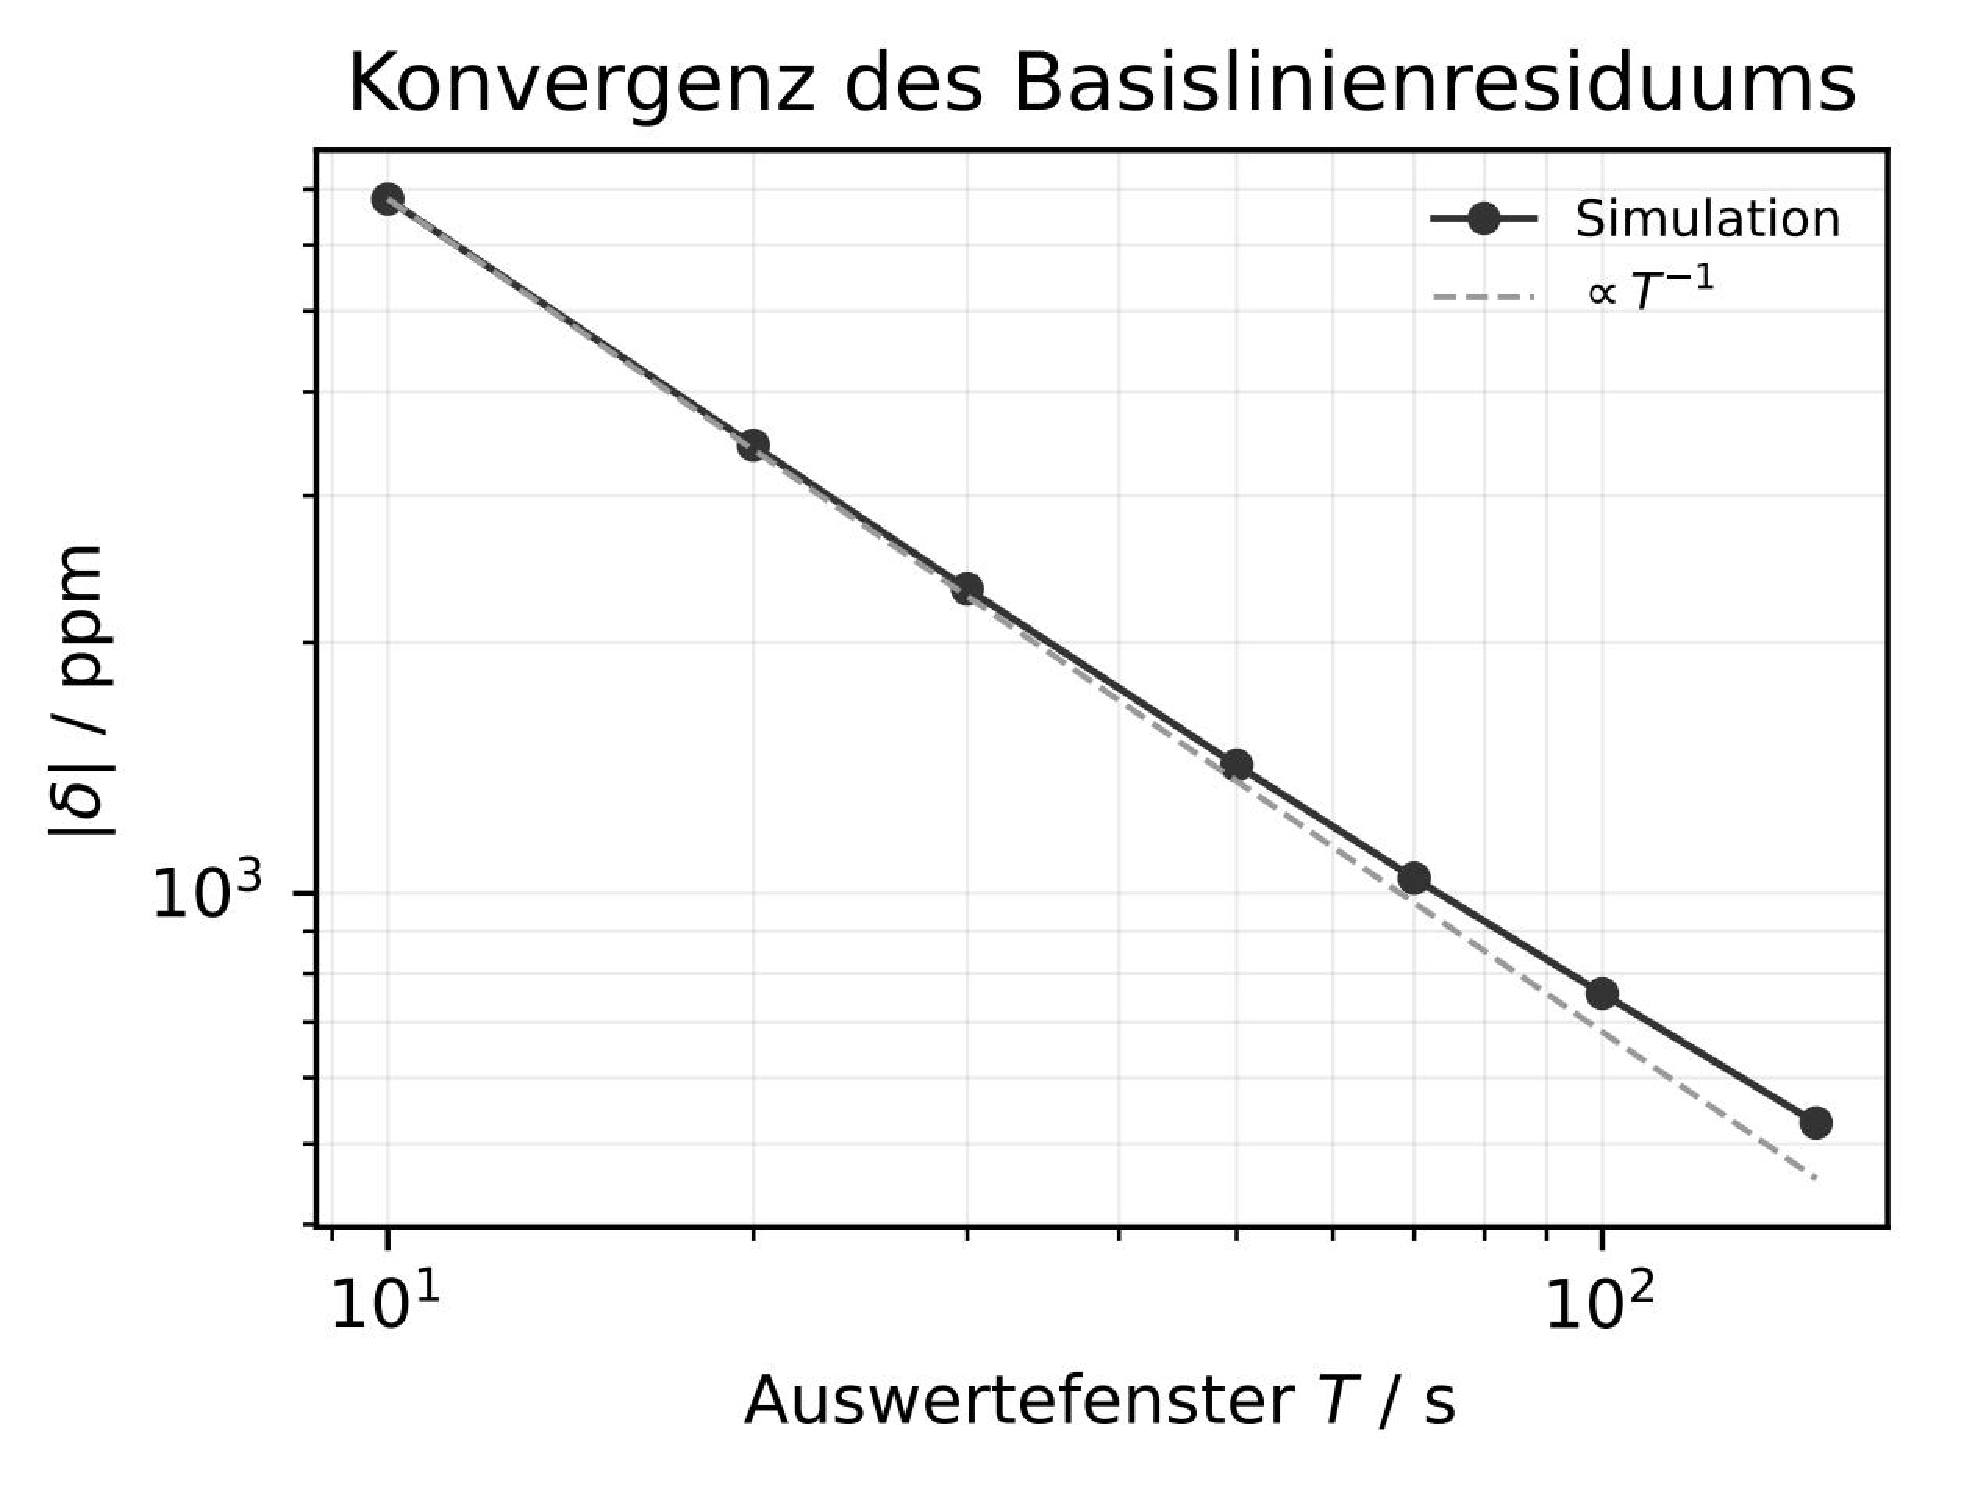
\includegraphics[width=0.72\textwidth]{Plots/konvergenz_residuum.pdf}
  \caption{Doppeltlogarithmische Darstellung des Residuums gegen die
  Fensterlänge. Der angepasste Exponent beträgt $-0{,}945$; die gestrichelte Gerade zeigt $\propto T_w^{-1}$. Die Achsenbeschriftung
  $T$ entspricht $T_w$.}
  \label{fig:konvergenz}
\end{figure}

Das Residuum fällt mit $T_w^{-0{,}945}$, also praktisch mit $T_w^{-1}$,
wie Gleichung~\eqref{eq:randterm} es für eine beschränkte
Geschwindigkeitsänderung verlangt. Ein Integrationsfehler, der je
Zeitschritt entsteht, bliebe von der Fensterlänge unabhängig. In der Kontrollkonfiguration mit
Dauerkontakt ist das Residuum bei $10\,\mathrm{s}$ wie bei
$70\,\mathrm{s}$ unverändert null.

Eine Nachrechnung aller $361$ Konfigurationen mit adaptivem Burn-in
trennt beide Anteile (Tabelle~\ref{tab:randterm}). Das Fenster wird dort
erst geöffnet, wenn die Zustände zu Zyklusbeginn wiederkehren. Der
Quadraturanteil bleibt überall unter $100\,\mathrm{ppm}$; jedes größere
Residuum ist Randterm.

\begin{table}[htbp]
  \centering
  \begin{tabular}{lr}
    \hline
    Größe & Wert \\
    \hline
    Konfigurationen mit $|\delta_w| \le 10\,\mathrm{ppm}$ (stationär) & 315 \\
    Konfigurationen mit $10 < |\delta_w| \le 100\,\mathrm{ppm}$ & 24 \\
    Konfigurationen mit $|\delta_w| > 100\,\mathrm{ppm}$ & 22 \\
    $\max |\delta_w|$ & $3714\,\mathrm{ppm}$ \\
    $\delta_Q$: Median; 5.\ bis 95.~Perzentil & $0$; $-51$ bis $+39\,\mathrm{ppm}$ \\
    $\max |\delta_Q|$ & $93\,\mathrm{ppm}$ \\
    \hline
  \end{tabular}
  \caption{Zerlegung des Residuums nach Gleichung~\eqref{eq:randterm}
  über $361$ Konfigurationen, Nachrechnung mit adaptivem Burn-in vom
  13.~September 2026, Fenster je $100$ Zyklen. Der größte Randterm liegt
  bei $(\varphi_2, \varphi_3) = (18{,}9^\circ, 303{,}2^\circ)$,
  $\lambda = 71{,}9\,\%$. Datensatz
  \texttt{sweep\_19x19\_burnin\_2026-09-13.csv}.}
  \label{tab:randterm}
\end{table}

Der Randterm hat drei Ursachen:

\begin{enumerate}
  \item \emph{Unvollständiges Einschwingen.} Der Archivlauf öffnete das
  Fenster nach festen $5\,\mathrm{s}$. An der Konfiguration von
  Tabelle~\ref{tab:konvergenz} dauert der Übergang $18{,}8\,\mathrm{s}$;
  danach liegt ein Orbit der Periode~1 vor, und der Randterm beträgt
  $-2\,\mathrm{ppm}$. Der Wert $-6816\,\mathrm{ppm}$ war Einschwingen.
  \item \emph{Fenster ohne ganze Orbitperioden.} Bei Orbits der
  Periode~3, 6 oder 30 verschwindet der Randterm, sobald das Fenster
  ganze Orbitperioden umfasst.
  \item \emph{Aperiodische Bewegung.} Hier bleibt $\delta_w$ bei jedem
  Fenster von der Ordnung $\Delta v_S/(g\,T_w)$, im Fenster von
  $10\,\mathrm{s}$ bis $0{,}37\,\%$.
\end{enumerate}

Eine langsame Modulation, wie sie frühere Fassungen als Ursache
annahmen, wird dafür nicht benötigt.

Die Kontrollgröße erfüllt damit genau die Funktion, die ihr in
Abschnitt~\ref{sec:baseline-and-observables} zugewiesen wurde: Sie hat einen Randterm des Auswertefensters sichtbar gemacht, die ohne bekannten
Sollwert als konfigurationsabhängiger Effekt erschienen wäre.

\begin{figure}[htbp]
  \centering
  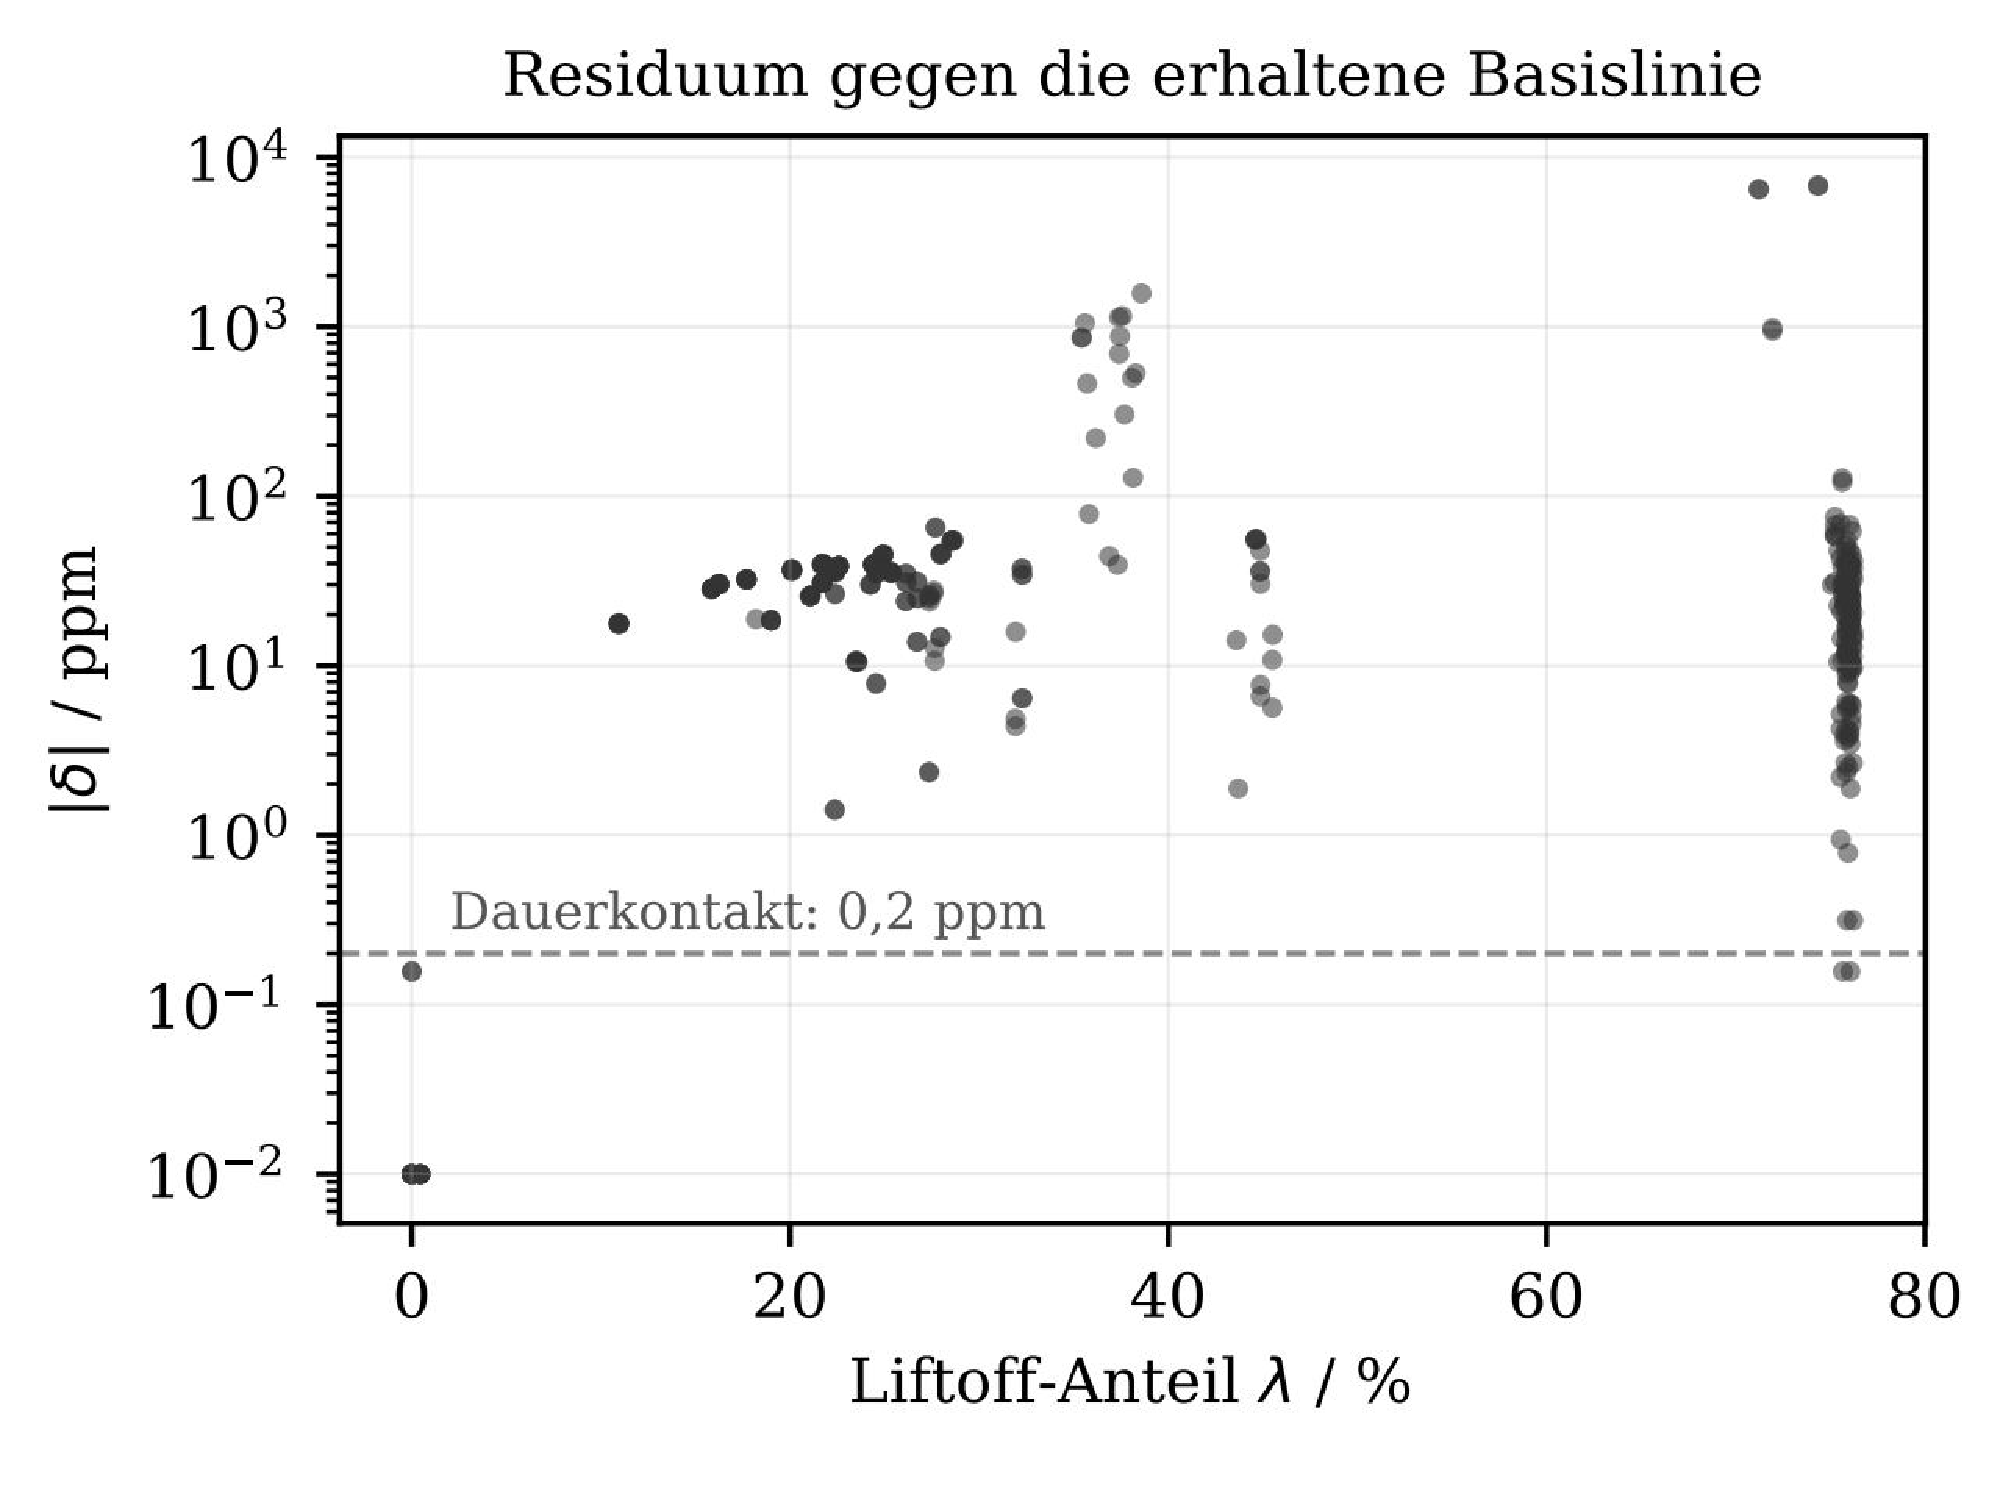
\includegraphics[width=0.72\textwidth]{Plots/residuum_liftoff.pdf}
  \caption{Betrag des relativen Residuums $|\delta|$ nach
  Gleichung~\eqref{eq:residual-def} gegen den Liftoff-Anteil, für alle 361 Konfigurationen des Archivlaufs (Burn-in fest $5\,\mathrm{s}$). Logarithmische Ordinate. Bei Dauerkontakt liegt
  das Residuum am numerischen Boden der Integration; mit wachsender
  Intermittenz steigt es um vier Größenordnungen.}
  \label{fig:residuum}
\end{figure}

\paragraph{Bezug zum zurückgezogenen Ergebnis.}
Eine frühere Phase dieses Projekts berichtete eine persistente
Mittelwertverschiebung der Kontaktkraft.
Tabelle~\ref{tab:residual-strat} ist die quantitative Signatur des dafür
verantwortlichen Mechanismus: ein konfigurationsabhängiger Randterm des Auswertefensters, der bei
Dauerkontakt verschwindet und bei starker Intermittenz den
Sub-Prozent-Bereich erreicht. Da der Liftoff-Anteil und mit ihm
Einschwingdauer und Periodizität von der Phasenkonfiguration abhängen,
erscheint dieser Randterm beim Vergleich von Konfigurationen über den
Intermittenzbereich hinweg als systematischer, phasenabhängiger Effekt
--- und ist doch nur die Impulsänderung über ein endliches, teils zu früh
geöffnetes Fenster. Auf dieser Grundlage wurde das frühere Ergebnis
zurückgezogen.

\paragraph{Folge für die Messkampagne.}
Daraus folgen drei Festlegungen. Erstens erfordern Konfigurationen mit
hohem Liftoff-Anteil eine gesonderte Auswertung der Kontrollgröße statt
einer gepoolten; eine einzelne aggregierte Kennzahl verdeckt die
Abhängigkeit und darf nicht als Qualifikationskriterium dienen.

Zweitens ist die Länge des Auswertefensters keine freie Wahl, sondern
eine Anforderung. Sie muss so bemessen sein, dass der Randterm nach Gleichung~\eqref{eq:randterm} unter die Nachweisschwelle fällt, und die
Konvergenz ist für die intermittenteste geprüfte Konfiguration
nachzuweisen, nicht anzunehmen. Die Wiederholung der Auswertung mit
verdoppeltem Fenster wird deshalb als Bestandteil der
Robustheitsprüfungen nach Kapitel~\ref{chap:statistik} geführt.

Drittens wird das Auswertefenster erst nach nachgewiesenem Einschwingen
geöffnet und bei periodischen Zuständen über ganze Orbitperioden gelegt;
die Schranke nach Gleichung~\eqref{eq:randterm} wird je Konfiguration
angegeben.

\section{Symmetrieprüfung}

Das Modell ist gegenüber der Vertauschung der beiden relativen Phasen
$(\varphi_2, \varphi_3) \rightarrow (\varphi_3, \varphi_2)$ invariant, da
die drei Module nominell identisch sind. Dies liefert eine zweite Prüfung
mit bekannter Antwort, unabhängig von der Basislinienprüfung.

Über die $171$ nichtdiagonalen Rasterpaare beträgt die mittlere Differenz
in $\langle N \rangle$ zwischen vertauschten Konfigurationen exakt null,
das Maximum $7{,}5\,\mathrm{mN}$. Die von null verschiedenen Fälle
konzentrieren sich in derselben Region hohen Liftoffs, die in
Abschnitt~\ref{sec:track1-sim} identifiziert wurde, was mit einem
numerischen statt einem strukturellen Ursprung vereinbar ist.

\section{Wertebereich der Zielfunktionale}
\label{sec:wertebereich}

Tabelle~\ref{tab:functional-range} gibt den Bereich an, über den die vier
Zielfunktionale über das Raster variieren. Diese Werte bilden die
Auslegungsgrundlage für die Spezifikation der Messtechnik.

\begin{table}[htbp]
  \centering
  \begin{tabular}{llrrr}
    \hline
    Funktional & Symbol & Minimum & Median & Maximum \\
    \hline
    Schiefe                 & $\gamma_1$   & $-0{,}288$ & $0{,}866$  & $1{,}979$ \\
    Liftoff-Anteil          & $\lambda$    & $0\,\%$    & $32{,}3\,\%$ & $76{,}2\,\%$ \\
    Asymmetrieverhältnis    & $A$          & $0{,}881$  & $2{,}445$  & $6{,}928$ \\
    Minimale Kraft          & $N_{\min}$   & $0$\,N     & $0$\,N     & $2{,}882$\,N \\
    Maximale Kraft          & $N_{\max}$   & $9{,}46$\,N & $21{,}97$\,N & $50{,}55$\,N \\
    \hline
  \end{tabular}
  \caption{Wertebereich der Zielfunktionale über 361
  Phasenkonfigurationen. Basislinie durchgehend
  $Mg = 6{,}3765\,\mathrm{N}$.}
  \label{tab:functional-range}
\end{table}

\begin{figure}[htbp]
  \centering
  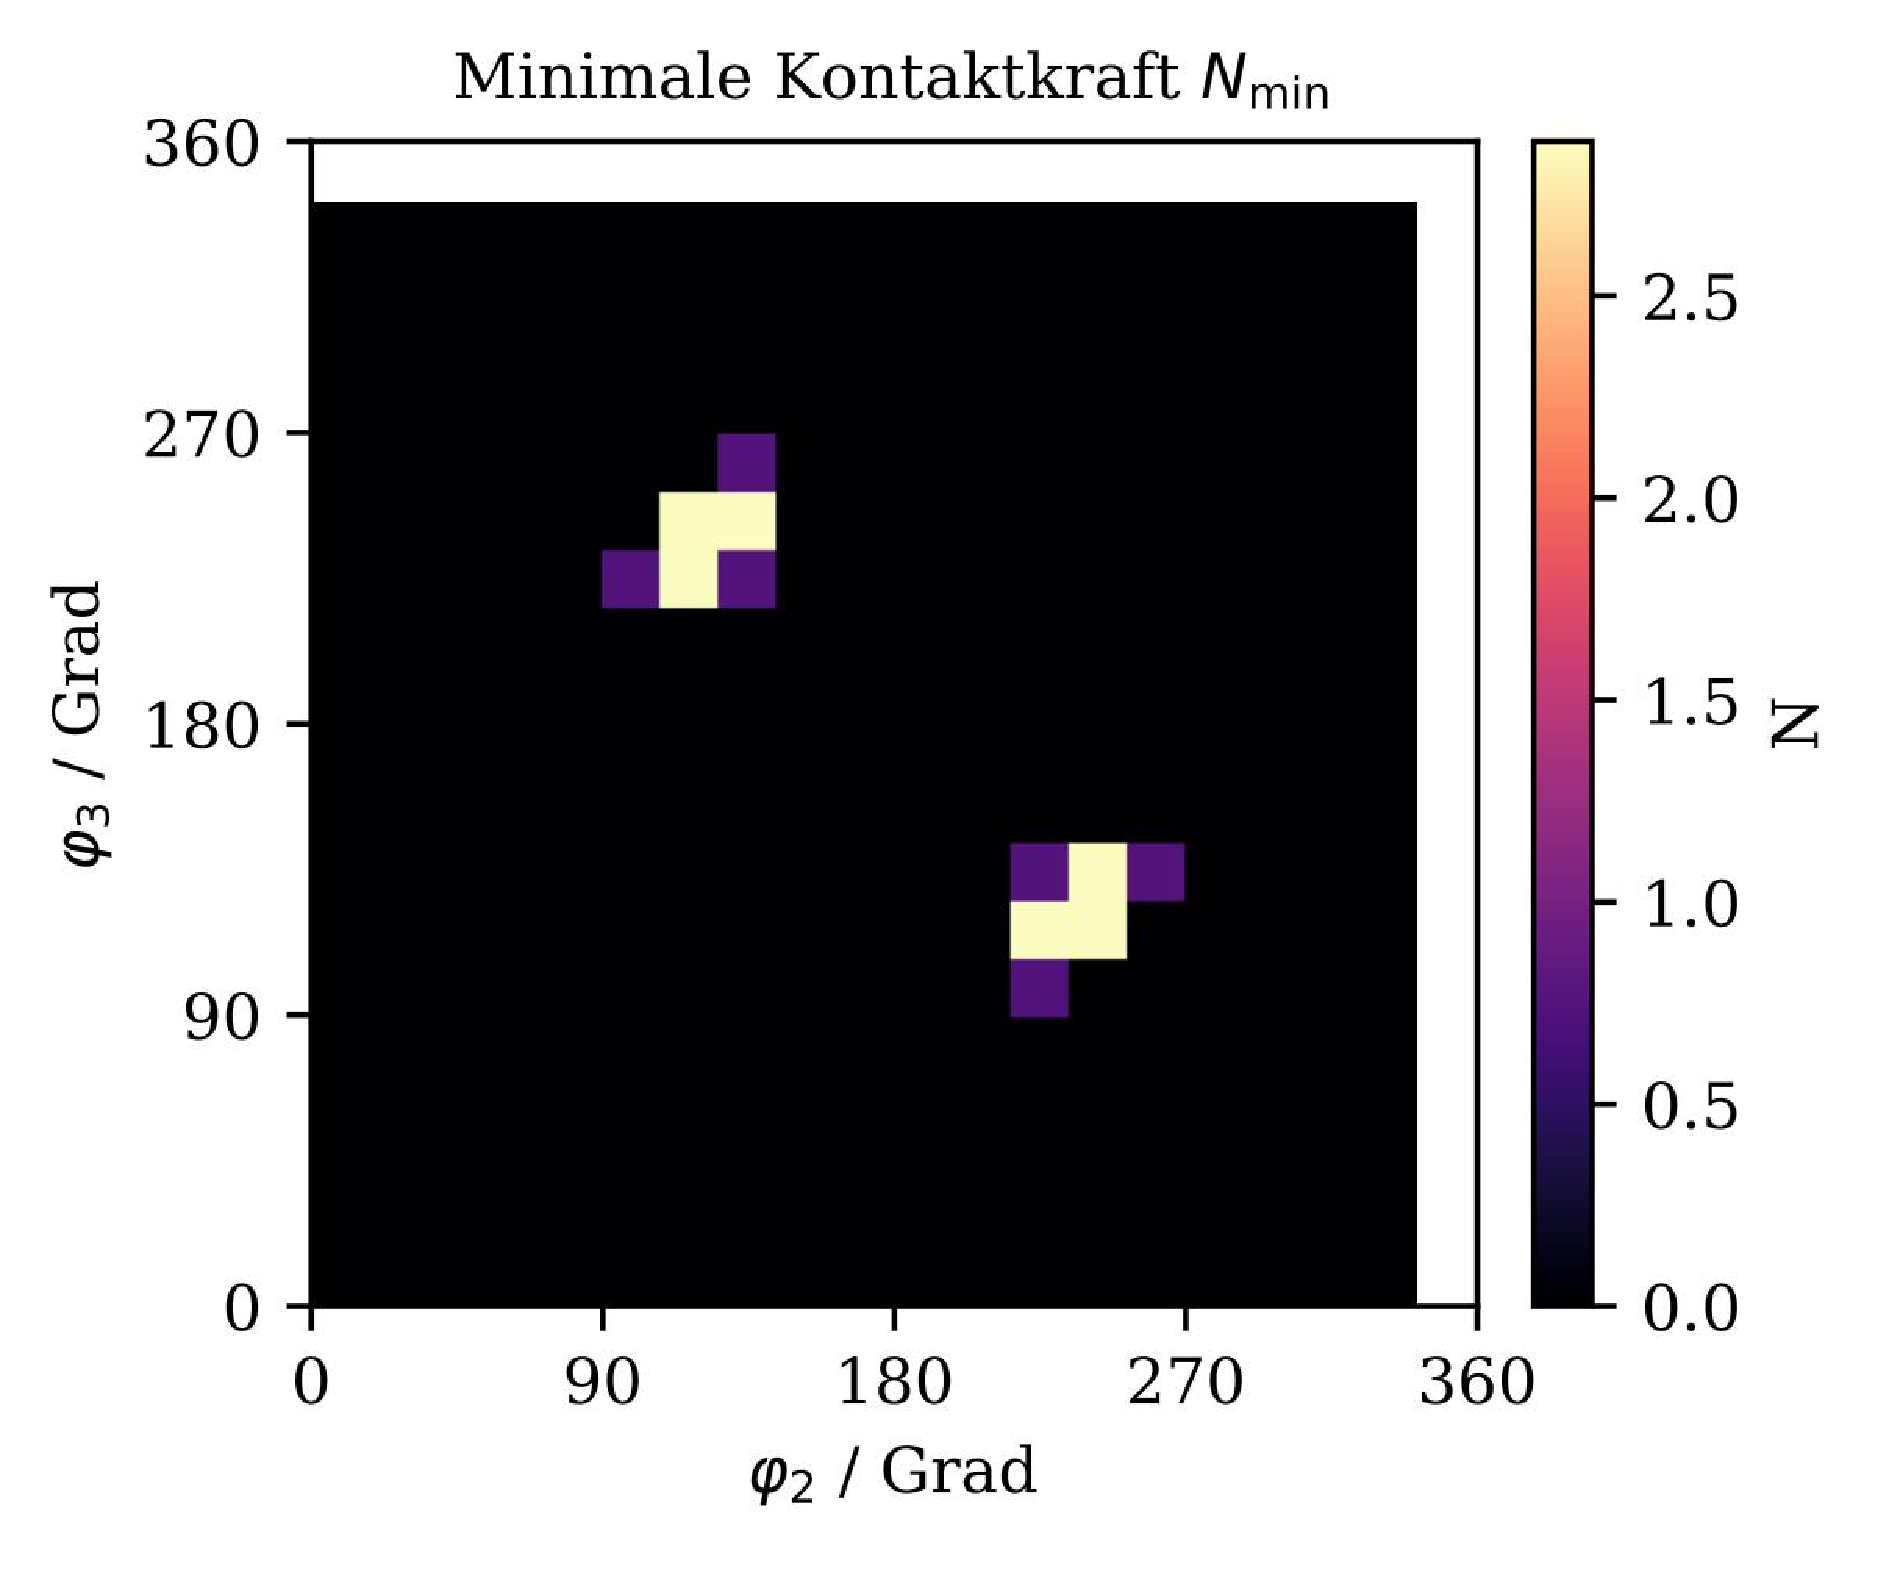
\includegraphics[width=0.48\textwidth]{Plots/karte_nmin.pdf}
  \hfill
  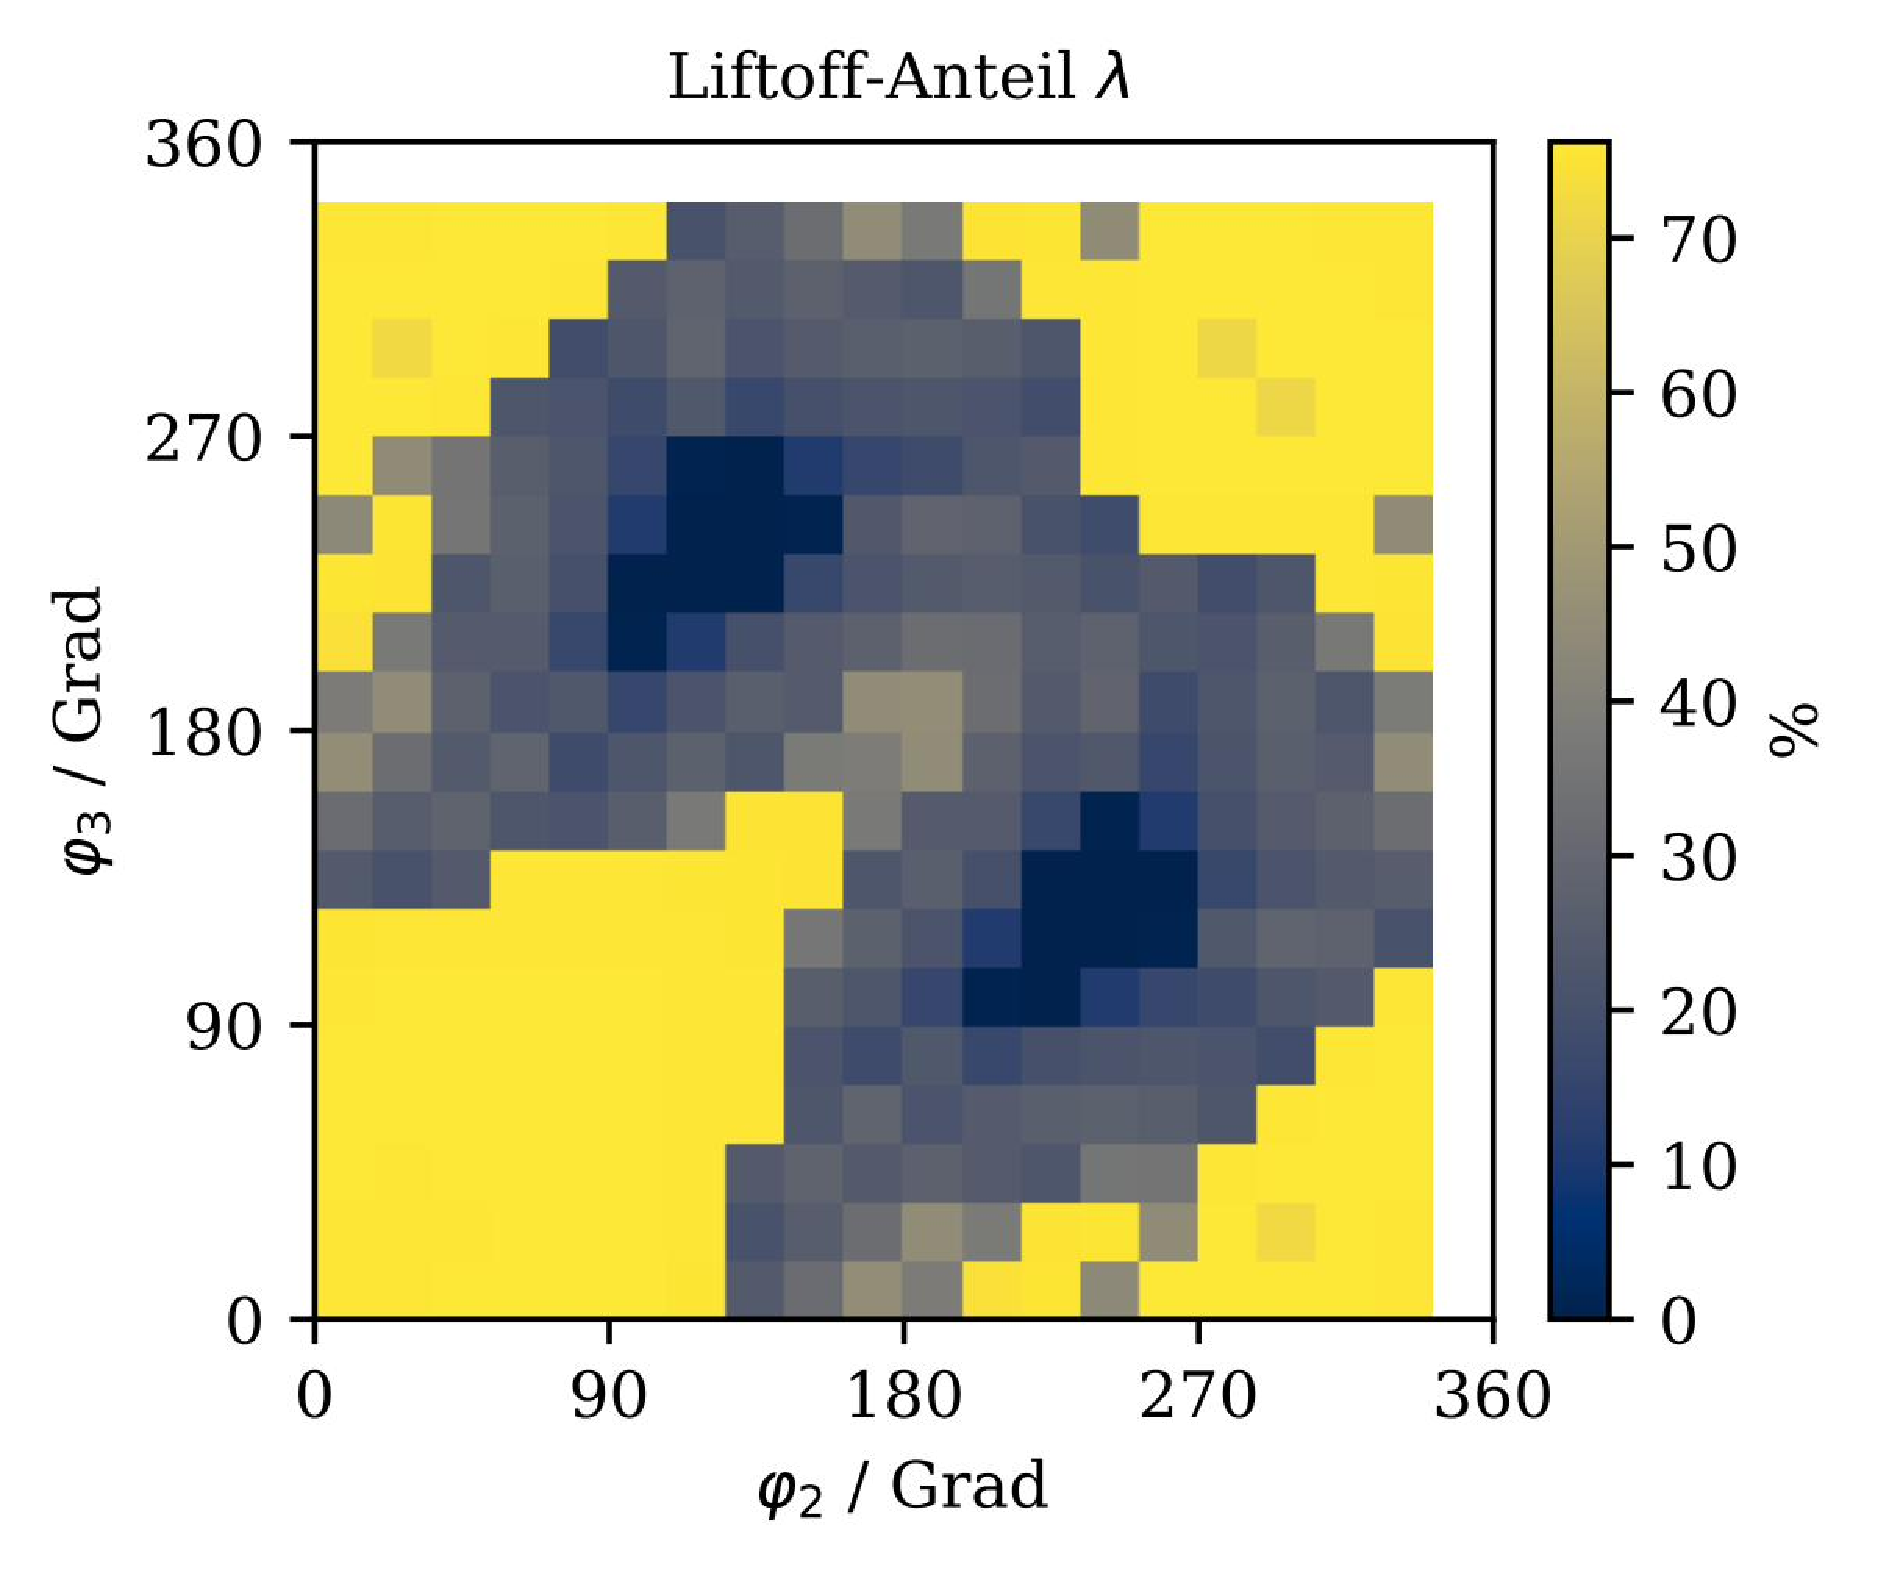
\includegraphics[width=0.48\textwidth]{Plots/karte_liftoff.pdf}\\[0.6em]
  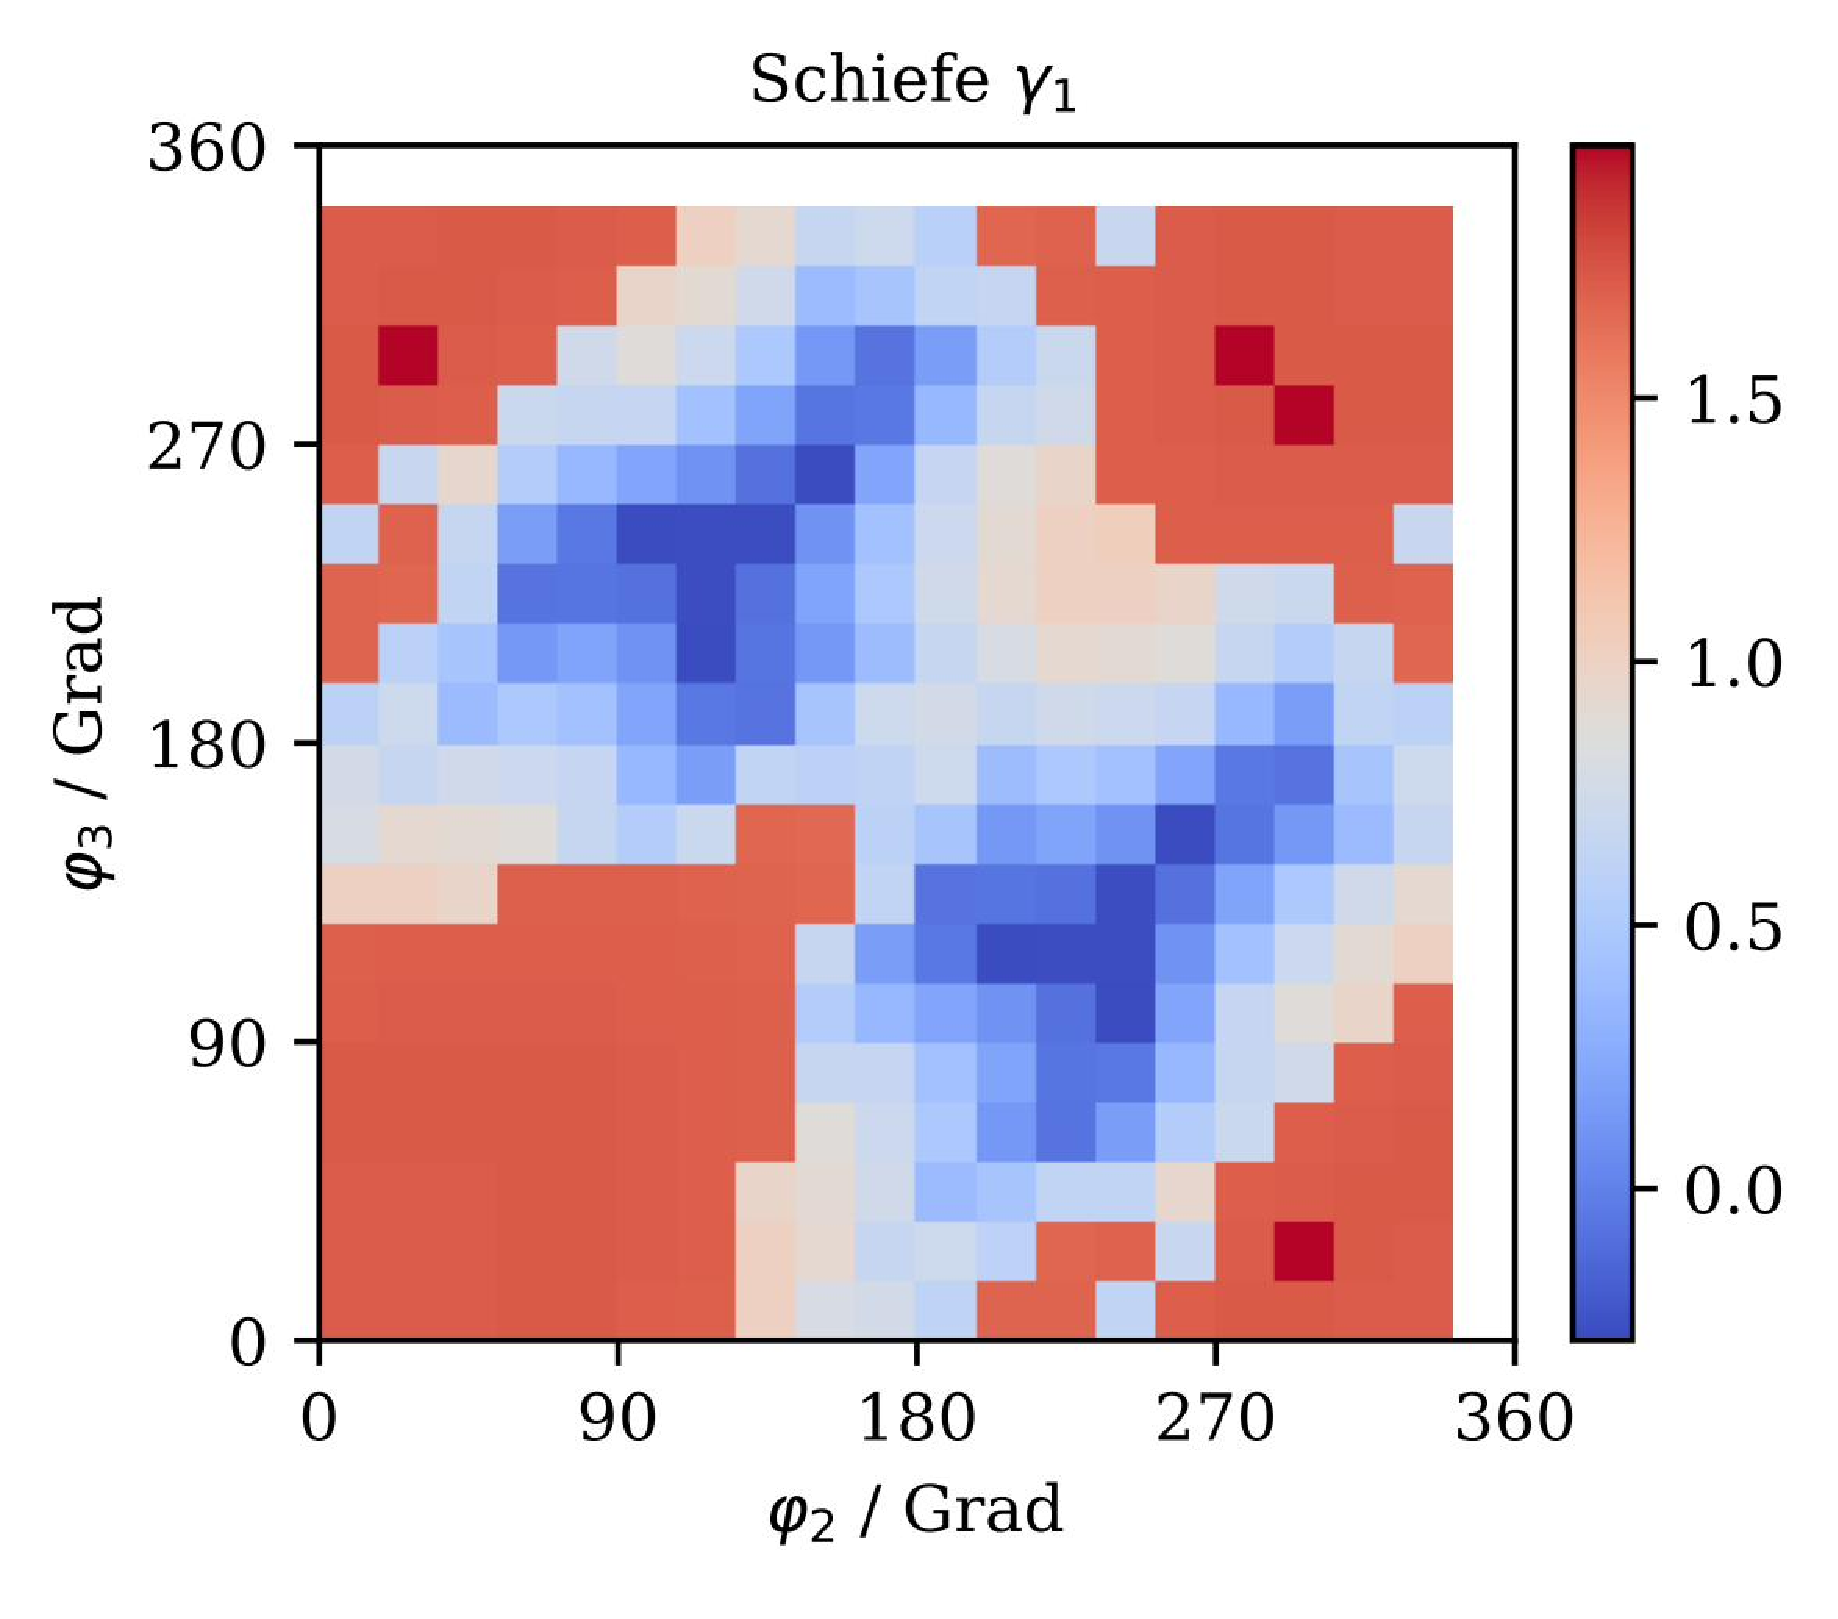
\includegraphics[width=0.48\textwidth]{Plots/karte_schiefe.pdf}
  \caption{Zielfunktionale über dem Raster der relativen
  Phasenkonfigurationen. Oben links die minimale Kontaktkraft
  $N_{\min}$, oben rechts der Liftoff-Anteil $\lambda$, unten die
  Schiefe $\gamma_1$. Die drei Karten zeigen dieselbe Struktur aus
  verschiedenen Blickwinkeln: Der Bereich mit $N_{\min} > 0$ ist genau
  der Bereich mit $\lambda = 0$.}
  \label{fig:karten}
\end{figure}

Zwei Merkmale sind für die Versuchsauslegung erheblich.

Erstens variieren die Funktionale um Faktoren und nicht um Prozente. Die
Spitzenkontaktkraft überstreicht über das Raster einen Faktor von $5{,}3$
und erreicht im Maximum das Achtfache der Basislinie, während das
Zeitmittel innerhalb von $0{,}07\,\%$ festliegt. Dies ist die
quantitative Form der Aussage, dass die Erhaltungsbedingung
ausschließlich das erste Moment betrifft.

Zweitens ist Dauerkontakt auf diesem Raster selten: Nur $12$ von $361$
Konfigurationen sind liftoff-frei, sämtlich mit
$\varphi_2 \in [94{,}7^\circ,\, 265{,}3^\circ]$. Innerhalb dieser
Teilmenge erreicht $N_{\min}$ den Wert $2{,}88\,\mathrm{N}$ bei
$(113{,}7^\circ,\, 227{,}4^\circ)$, dem Rasterpunkt, der der
triphasischen Konfiguration am nächsten liegt.
Abbildung~\ref{fig:schnitt} zeigt den zugehörigen Schnitt.

\begin{figure}[htbp]
  \centering
  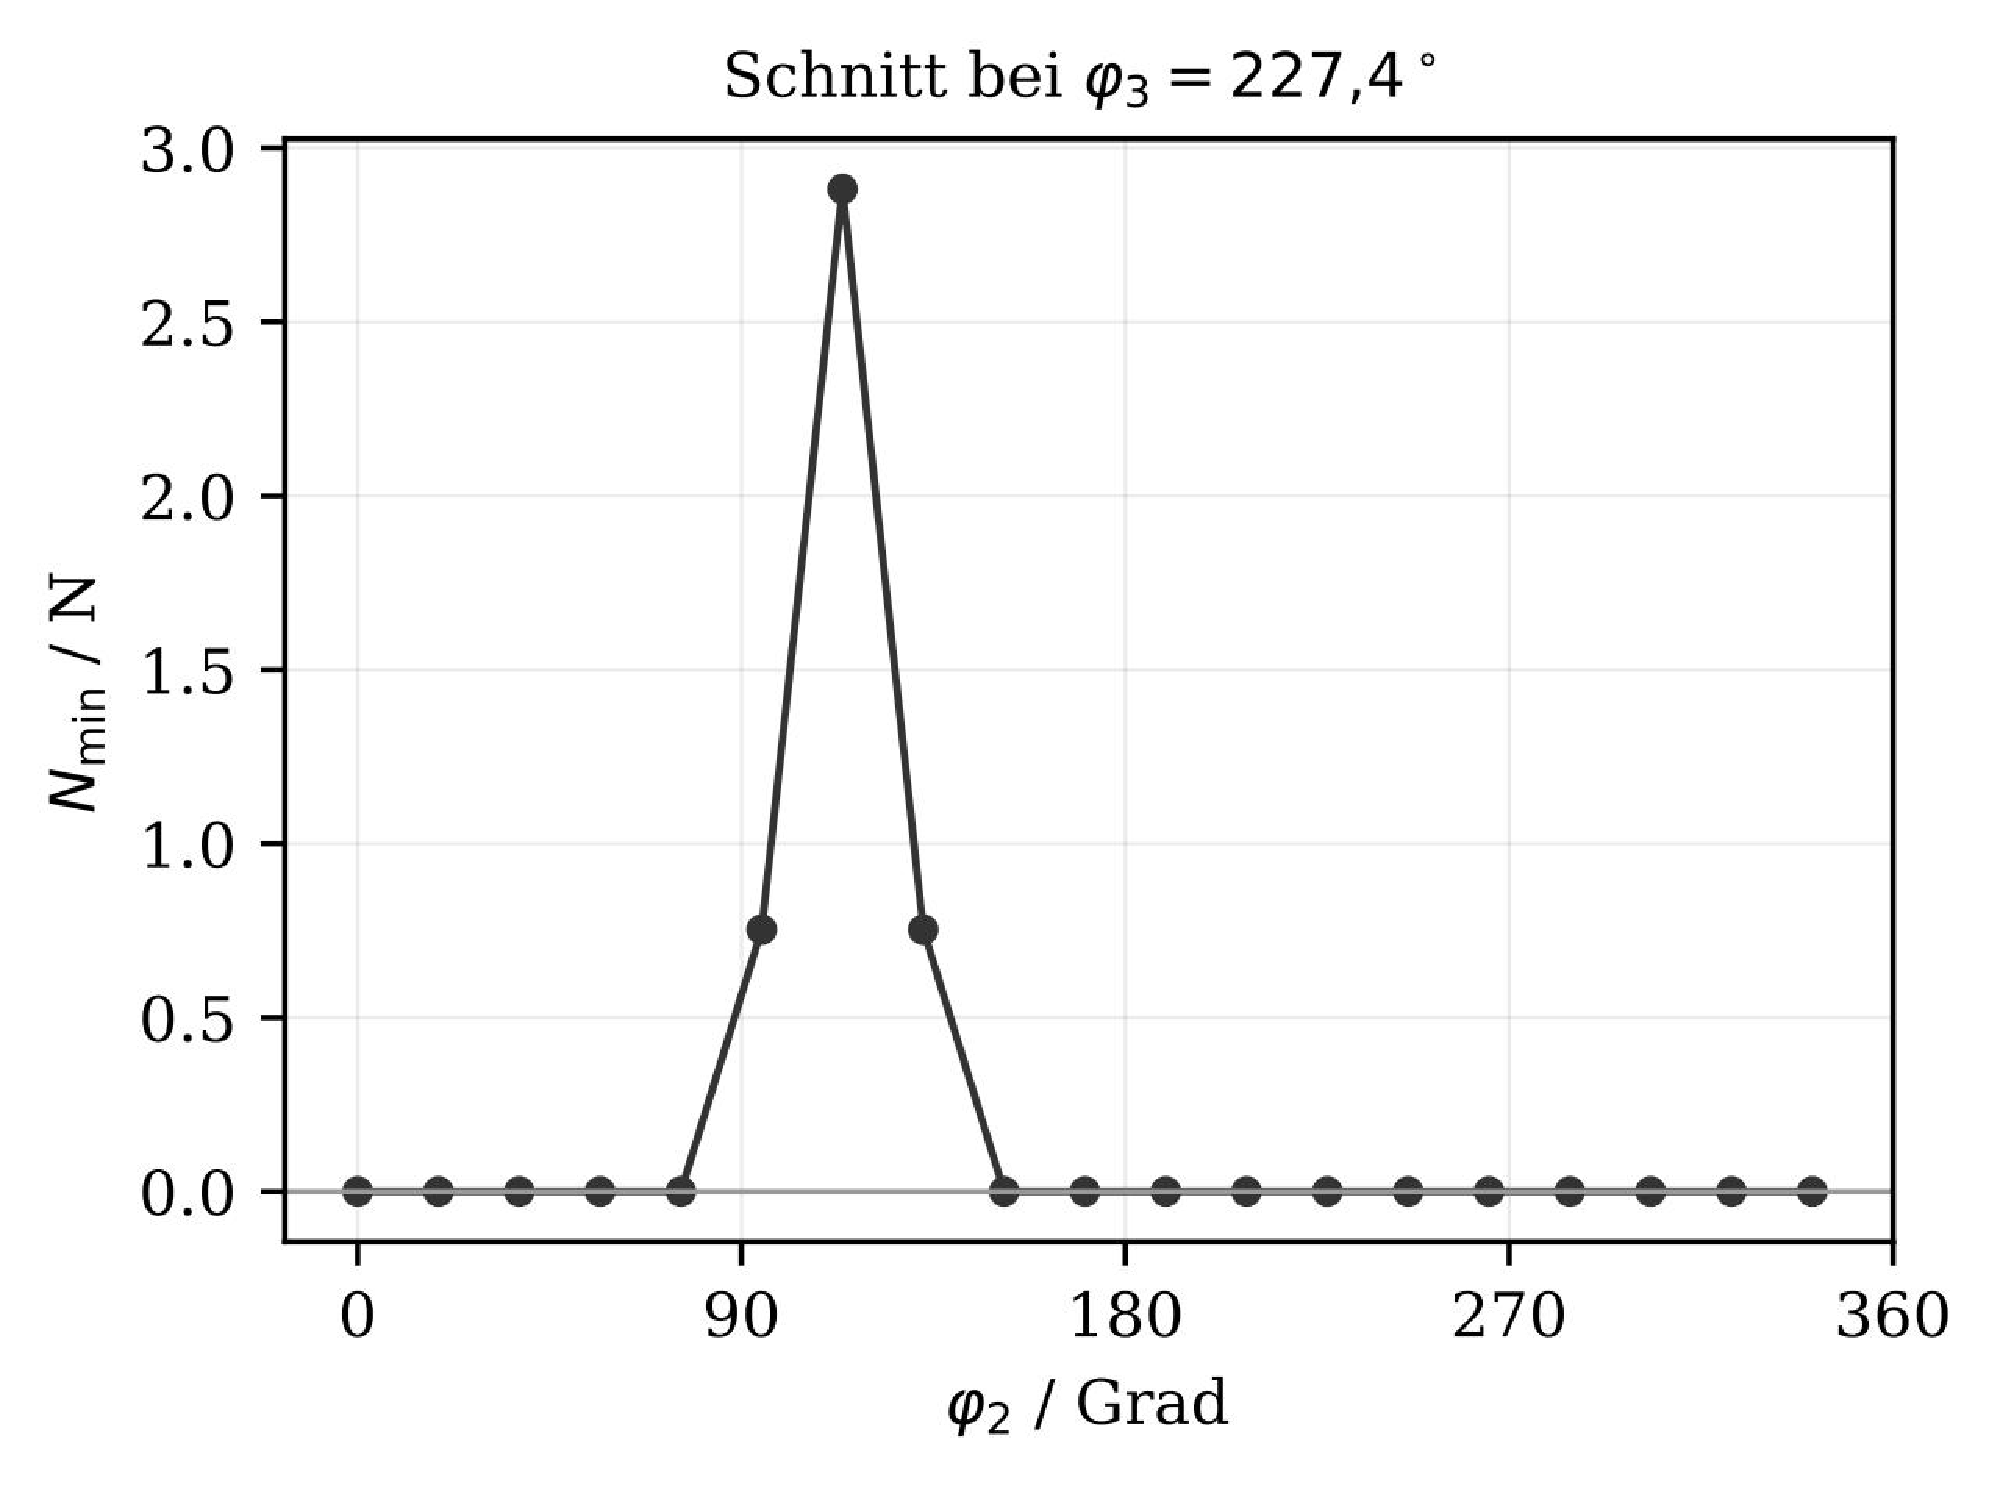
\includegraphics[width=0.72\textwidth]{Plots/schnitt_nmin.pdf}
  \caption{Minimale Kontaktkraft entlang $\varphi_2$ bei festem
  $\varphi_3 = 227{,}4^\circ$. Drei der neunzehn Rasterpunkte dieses
  Schnitts sind liftoff-frei. Die Rasterweite von $18{,}9^\circ$ löst
  den Verlauf zwischen ihnen nicht auf.}
  \label{fig:schnitt}
\end{figure}

Das Grobraster löst das Innere dieser Region nicht auf: Von den neunzehn
Punkten des Schnitts liegen nur drei im Dauerkontakt, und die Rasterweite
von $18{,}9^\circ$ ist größer als die Breite der Struktur, die sie
abbilden soll. Eine feinere Abtastung liegt inzwischen vor: ein Sweep mit
$2^\circ$-Raster über $\varphi_2 \in [100^\circ, 140^\circ]$ und
$\varphi_3 \in [220^\circ, 260^\circ]$, also $441$ Konfigurationen, mit
derselben Engine und demselben Parametersatz wie
Tabelle~\ref{tab:sim-params} (Datensatz
\texttt{finesweep\_2deg\_120\_240.csv} im Repository-Stand 2026-09
\cite{frueh2026repo}). Die minimale Kontaktkraft bildet dort eine
Zeltkurve mit Spitze $N_{\min} = 5{,}3304\,\mathrm{N}$ genau am
triphasischen Punkt $(120^\circ, 240^\circ)$. Entlang $\varphi_3 =
240^\circ$ fällt sie mit etwa $0{,}23\,\mathrm{N}$ je Grad zu kleineren
und etwa $0{,}19\,\mathrm{N}$ je Grad zu größeren $\varphi_2$ ab; die
Zeltkurve ist also nicht symmetrisch. $400$ der $441$ Konfigurationen,
$90{,}7\,\%$ des Fensters, sind liftoff-frei, und
$|\langle N \rangle - Mg| \le 0{,}2\,\mathrm{mN}$ gilt im gesamten
Fenster. Der Feinsweep bestätigt damit den Befund des Grobrasters und
liefert die Breite der Dauerkontaktregion, die das $18{,}9^\circ$-Raster
nicht auflöst.

\section{Sweep mit sinusförmigem Bahnprofil}
\label{sec:sinus-sweep}

Die kostengünstige Laborvariante treibt die Modulmassen mit Exzenter oder
Kurbel an (Kapitel~\ref{chap:system}). Ein Exzenter mit Flachstößel
erzeugt eine exakt sinusförmige Bewegung, eine Schubkurbel eine
näherungsweise sinusförmige mit schwacher zweiter Harmonischer. Beides
unterscheidet sich grundlegend vom asymmetrischen Profil des
Simulationsmodells mit langsamer Halte- und schneller Rückholphase. Um
zu prüfen, ob die Vorhersagen dieses Kapitels den Übergang zum
sinusförmigen Antrieb überstehen, wurde der Sweep mit einem
sinusförmigen Profil gleichen Hubs wiederholt: Spitze-Spitze
$7{,}69\,\mathrm{mm}$, Amplitude $A = 3{,}85\,\mathrm{mm}$, alle übrigen
Parameter unverändert. Ein $7\times7$-Raster mit Schrittweite
$51{,}4^\circ$ genügt, aus einem Grund, der sich aus dem Ergebnis selbst
ergibt.

\paragraph{Kollaps auf einen Parameter.}
Drei gleichfrequente Sinusschwingungen mit den relativen Phasen
$0$, $\varphi_2$, $\varphi_3$ addieren sich zu einer einzigen
Sinusschwingung,

\begin{equation}
\sum_{k} \sin(\omega t - \varphi_k)
= R\,\sin(\omega t - \psi),
\qquad
R = \bigl|\,1 + e^{i\varphi_2} + e^{i\varphi_3}\,\bigr| .
\label{eq:R}
\end{equation}

Der Rahmen erfährt damit eine sinusförmige Trägheitskraft der Amplitude
$M A \omega^{2} R / 3$, und die gesamte Phasenkonfiguration wirkt
ausschließlich über den Betrag $R \in [0, 3]$. Die zweidimensionale
Phasenkarte degeneriert zu einer einparametrigen Schar.
Tabelle~\ref{tab:sinus-kollaps} bestätigt dies numerisch: Rasterpunkte mit
gleichem $R$ liefern identische Observablen.

\begin{table}[htbp]
  \centering
  \begin{tabular}{rrrrr}
    \hline
    $R$ & Punkte & $\gamma_1$ & $\lambda$ / \% & Streuung von $\gamma_1$ \\
    \hline
    0{,}555 & 6  & 0{,}000 & 0{,}0  & $< 10^{-4}$ \\
    0{,}802 & 6  & 0{,}000 & 0{,}0  & $< 10^{-4}$ \\
    1{,}182 & 6  & 0{,}000 & 0{,}0  & $< 10^{-4}$ \\
    1{,}414 & 12 & 0{,}000 & 0{,}0  & $< 10^{-4}$ \\
    2{,}027 & 6  & 1{,}707 & 76{,}0 & $< 10^{-4}$ \\
    2{,}247 & 6  & 1{,}823 & 73{,}8 & 0{,}081 \\
    2{,}738 & 6  & 1{,}687 & 75{,}2 & 0{,}0002 \\
    \hline
  \end{tabular}
  \caption{Sinusförmiges Profil, $7\times7$-Raster: Observablen
  gruppiert nach der resultierenden Amplitude $R$. Innerhalb jeder
  Gruppe fallen die Werte zusammen; die einzige nennenswerte Streuung
  bei $R = 2{,}25$ stammt aus dem stark intermittierenden Bereich.}
  \label{tab:sinus-kollaps}
\end{table}

\begin{figure}[htbp]
  \centering
  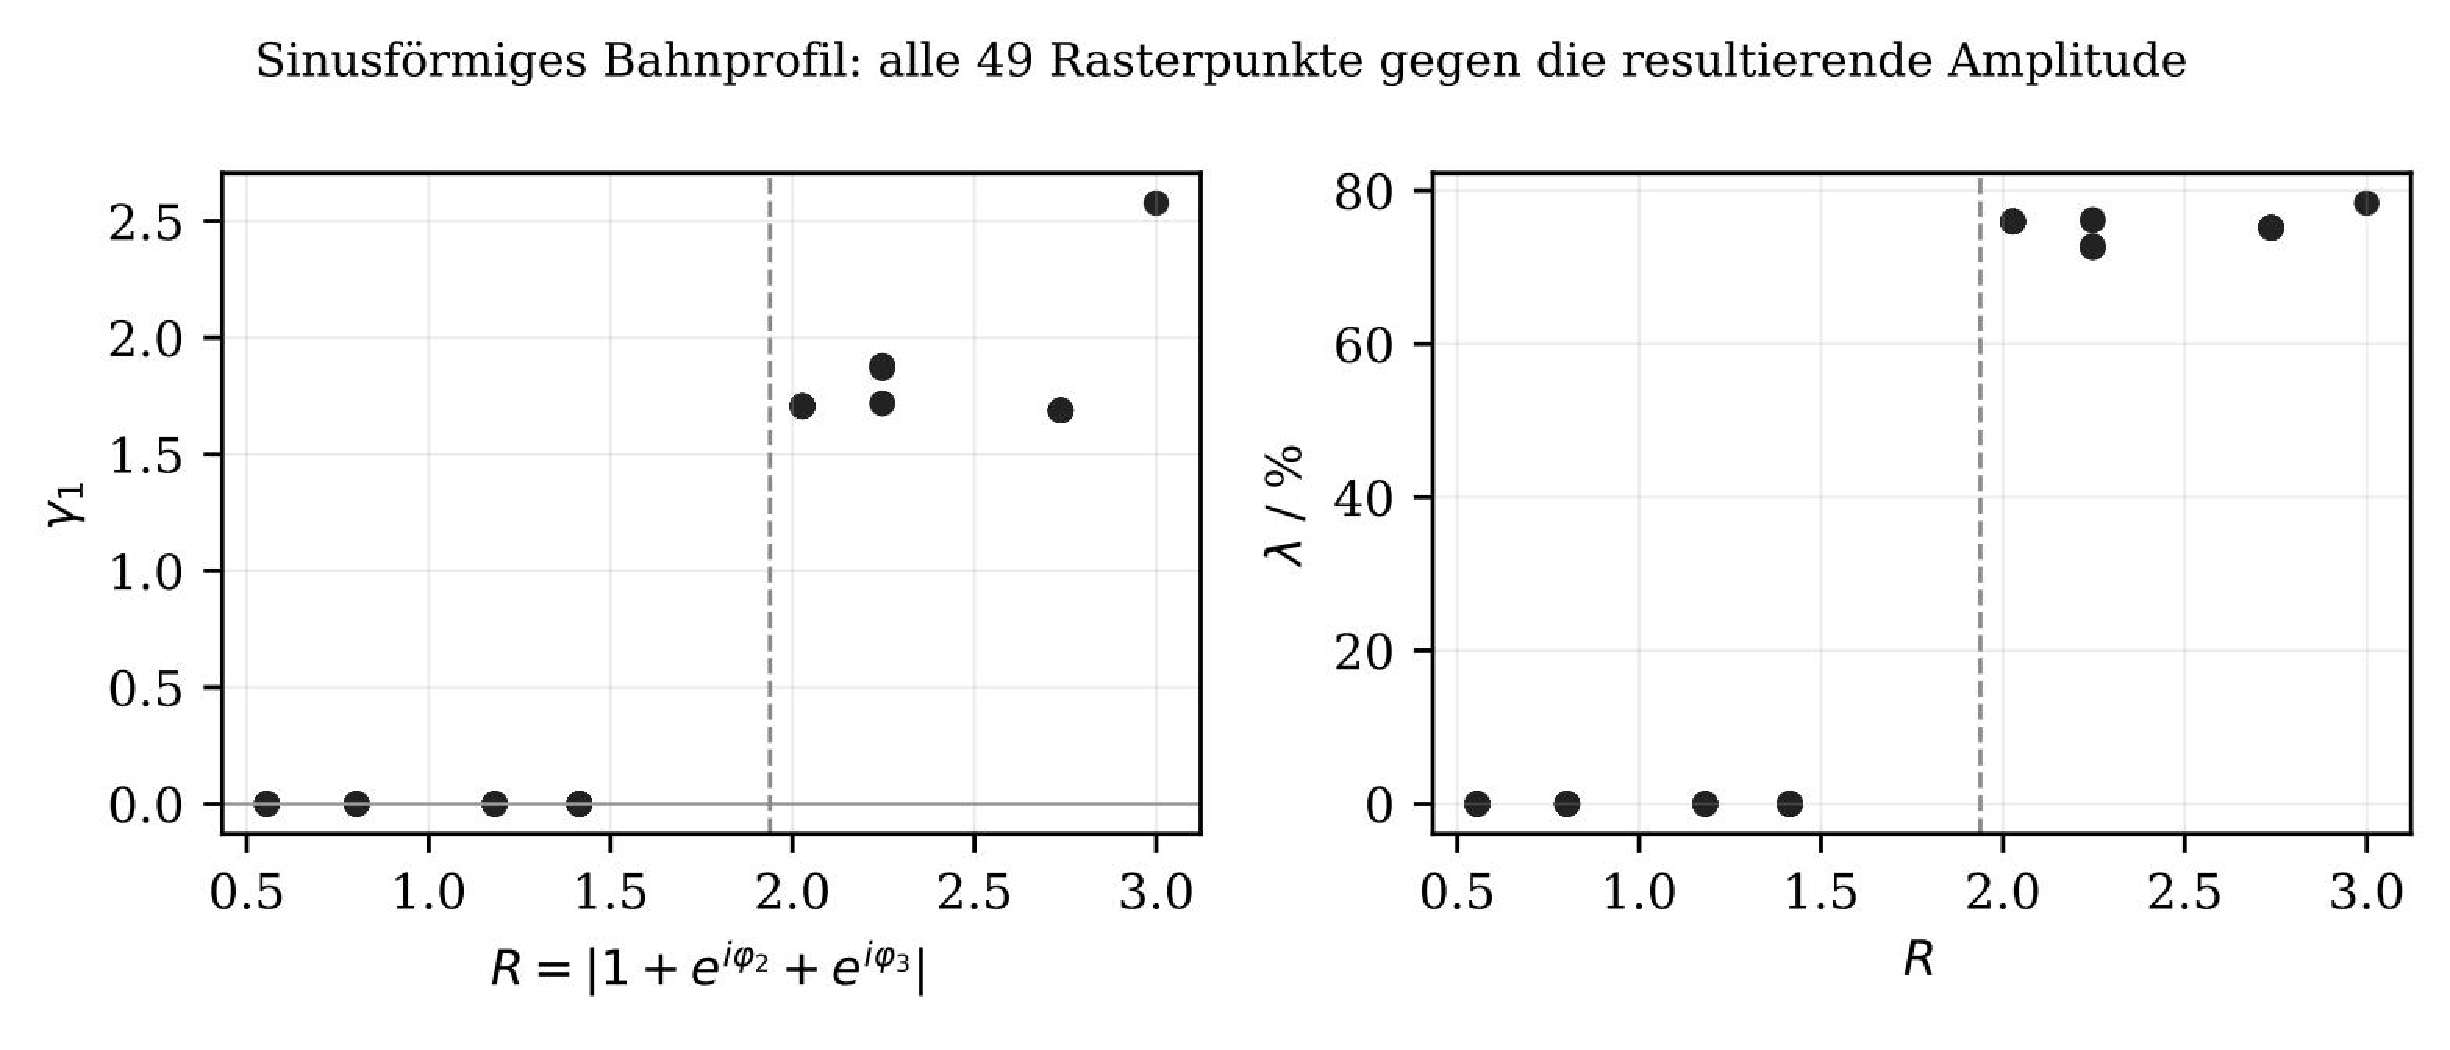
\includegraphics[width=0.9\textwidth]{Plots/sinus_kollaps.pdf}
  \caption{Alle 49 Rasterpunkte des Sinus-Sweeps gegen $R$. Links die
  Schiefe, rechts der Liftoff-Anteil. Gestrichelt die quasistatische
  Schwelle $R_c^{\mathrm{qs}} = 1{,}94$; die tatsächliche Schwelle liegt
  nach Gleichung~\eqref{eq:Rc-dyn} bei $1{,}45$.}
  \label{fig:sinus-kollaps}
\end{figure}

\paragraph{Liftoff-Schwelle.}
Auf starrer Unterlage hebt der Kontakt ab, sobald die
Trägheitsbeschleunigung die Erdbeschleunigung übersteigt,
$A \omega^{2} R / 3 > g$, also für

\begin{equation}
R > R_c^{\mathrm{qs}} = \frac{3g}{A\omega^{2}} = 1{,}94 .
\label{eq:Rc}
\end{equation}

Das ist die quasistatische Schwelle, und sie gilt hier nicht. Der
Kontakt ist nachgiebig; mit $r = f/f_n = 0{,}51$ und $\zeta = 0{,}10$
überträgt er die Trägheitskraft mit der Transmissibilität

\begin{equation}
T = \sqrt{\frac{1 + (2\zeta r)^{2}}{(1-r^{2})^{2} + (2\zeta r)^{2}}} = 1{,}34 ,
\label{eq:transmissibilitaet}
\end{equation}

so dass die Kontaktkraft stärker schwankt als auf starrer Unterlage und
die Schwelle entsprechend früher erreicht wird:

\begin{equation}
R_c = \frac{R_c^{\mathrm{qs}}}{T} = 1{,}45 .
\label{eq:Rc-dyn}
\end{equation}

Eine feine Abtastung entlang der Diagonale $\varphi_2 = \varphi_3$
bestätigt dies: Bei $R = 1{,}44$ erreicht die minimale Kontaktkraft mit
$0{,}005\,Mg$ gerade noch nicht null, bei $R = 1{,}48$ hebt der Kontakt
während $8{,}5\,\%$ des Zyklus ab. Die Schwelle liegt damit zwischen
$1{,}44$ und $1{,}48$, in Übereinstimmung mit
Gleichung~\eqref{eq:Rc-dyn} und $34\,\%$ unterhalb der quasistatischen
Formel. Von den 49 Rasterpunkten bleiben 30 im Dauerkontakt.

Oberhalb der Schwelle wächst der Liftoff-Anteil zunächst langsam ---
$8{,}5\,\%$ bei $R = 1{,}48$, $18\,\%$ bei $R = 1{,}62$ --- und springt
zwischen $R = 1{,}62$ und $1{,}70$ auf $75\,\%$. Der Übergang vom
kurzzeitigen Abheben zum prellenden Betrieb ist also kein stetiger,
sondern ein Umschlag.

\paragraph{Schiefe.}
Unterhalb der Schwelle ist die Kontaktkraft eine reine Sinusschwingung
um $Mg$ und damit symmetrisch verteilt: $\gamma_1 = 0$ in allen 30
liftoff-freien Konfigurationen, auf vier Nachkommastellen. Oberhalb der
Schwelle ist $\gamma_1$ positiv, zwischen $+1{,}69$ und $+2{,}58$.
\textbf{Negative Schiefe tritt mit sinusförmigem Profil nirgends auf.}

\paragraph{Spitzenkraft.}
Im synchronen Fall $R = 3$ erreicht die Spitzenkontaktkraft das
$13{,}6$-fache der Basislinie, rund $87\,\mathrm{N}$ --- deutlich mehr
als die $7{,}9\,Mg$ des asymmetrischen Profils, weil sich drei
Sinusschwingungen kohärent addieren, während sich drei asymmetrische
Profile bei jeder Phasenlage teilweise verteilen.

\paragraph{Folgerung.}
Das Ergebnis ist eindeutig und für die Versuchsauslegung bindend. Mit
sinusförmigem Antrieb ist das Dreimodulsystem einem einzelnen
Schwingerreger mit einstellbarer Amplitude äquivalent. Die
Phasenkonfiguration $(\varphi_2, \varphi_3)$ trägt dann keine
Information, die nicht in $R$ enthalten wäre; ein Raster über der
Phasenebene misst dieselbe eindimensionale Kurve vielfach. Die
Vorhersage zum Vorzeichen der Schiefe nach
Abschnitt~\ref{sec:vorhersage-schiefe} ist mit diesem Antrieb nicht
prüfbar, weil der Fall $\gamma_1 < 0$ nicht auftritt. Und die
Anordnung reproduziert im Ergebnis das Experiment von Rigaud und
Perret-Liaudet \cite{rigaud2003} --- harmonisch angeregter unilateraler
Kontakt mit variabler Amplitude --- statt die in
Kapitel~\ref{chap:stand} benannte Lücke zu adressieren.

Die Asymmetrie des Bahnprofils ist demnach kein Detail der Umsetzung,
sondern die Quelle der gesamten Phasenabhängigkeit jenseits der
Amplitude. Für die Laborvariante folgt: Ein Antrieb, der ein asymmetrisches Profil
erzeugt --- Nocke oder programmierbarer Aktor ---, ist zwingend;
Exzenter und Kurbel bei konstanter Drehzahl scheiden aus. Der Sinus-Sweep behält
dennoch einen Nutzen: Er ist die Referenz, gegen die der Beitrag der
Profilasymmetrie in der Messung beziffert werden kann, und er liefert
mit Gleichung~\eqref{eq:Rc-dyn} eine aus Transmissibilität und
Hub berechenbare Liftoff-Schwelle als zusätzliche Prüfgröße mit
bekannter Antwort.

\section{Sensitivität gegenüber Steifigkeit und Dämpfung}
\label{sec:sens-k}

Alle bisherigen Ergebnisse dieses Kapitels gelten für einen einzigen
Kontaktparametersatz, $k = 10^{4}\,\mathrm{N/m}$ und
$c = 16\,\mathrm{N\,s/m}$. Da die Steifigkeit des Kontaktelements in der
Laborvariante frei wählbar ist --- Elastomerpad, Feder, Metallauflage ---
wurde der Sweep für fünf Steifigkeiten über zwei Dekaden wiederholt, bei
festem Dämpfungsgrad $\zeta = 0{,}10$ und unverändertem asymmetrischem
Profil. Je Steifigkeit ein $7\times7$-Raster; die Vergleichbarkeit mit
dem $19\times19$-Raster ist entsprechend eingeschränkt.

\begin{table}[htbp]
  \centering
  \resizebox{\textwidth}{!}{%
\begin{tabular}{rrrrrrrr}
    \hline
    $k$ / N/m & $f_n$ / Hz & $3f/f_n$ & liftoff-frei & $\max\lambda$ / \% & $\min\gamma_1$ & $\max N_{\max}/Mg$ & $\gamma_1{<}0$ bei Paar \\
    \hline
    $10^{3}$          &  6{,}2 & 4{,}81 & 48 & 12{,}4 & $-0{,}331$ &  1{,}94 & 16 von 34 \\
    $3\cdot10^{3}$    & 10{,}8 & 2{,}77 &  0 & 56{,}7 & $+0{,}361$ &  3{,}52 & 0 von 0 \\
    $10^{4}$          & 19{,}7 & 1{,}52 &  0 & 76{,}1 & $-0{,}128$ &  7{,}09 & 0 von 6 \\
    $3\cdot10^{4}$    & 34{,}2 & 0{,}88 & 18 & 86{,}2 & $-0{,}495$ & 13{,}96 & 0 von 12 \\
    $10^{5}$          & 62{,}4 & 0{,}48 & 30 & 92{,}1 & $-0{,}945$ & 26{,}05 & 0 von 18 \\
    \hline
  \end{tabular}%
}
  \caption{Sensitivität gegenüber der Kontaktsteifigkeit, je
  $7\times7$-Raster, $\zeta = 0{,}10$. Letzte Spalte: Zahl der
  Konfigurationen mit negativer Schiefe, in denen zwei Module gleichphasig
  laufen, bezogen auf alle Konfigurationen mit negativer Schiefe.}
  \label{tab:sens-k}
\end{table}

\begin{figure}[htbp]
  \centering
  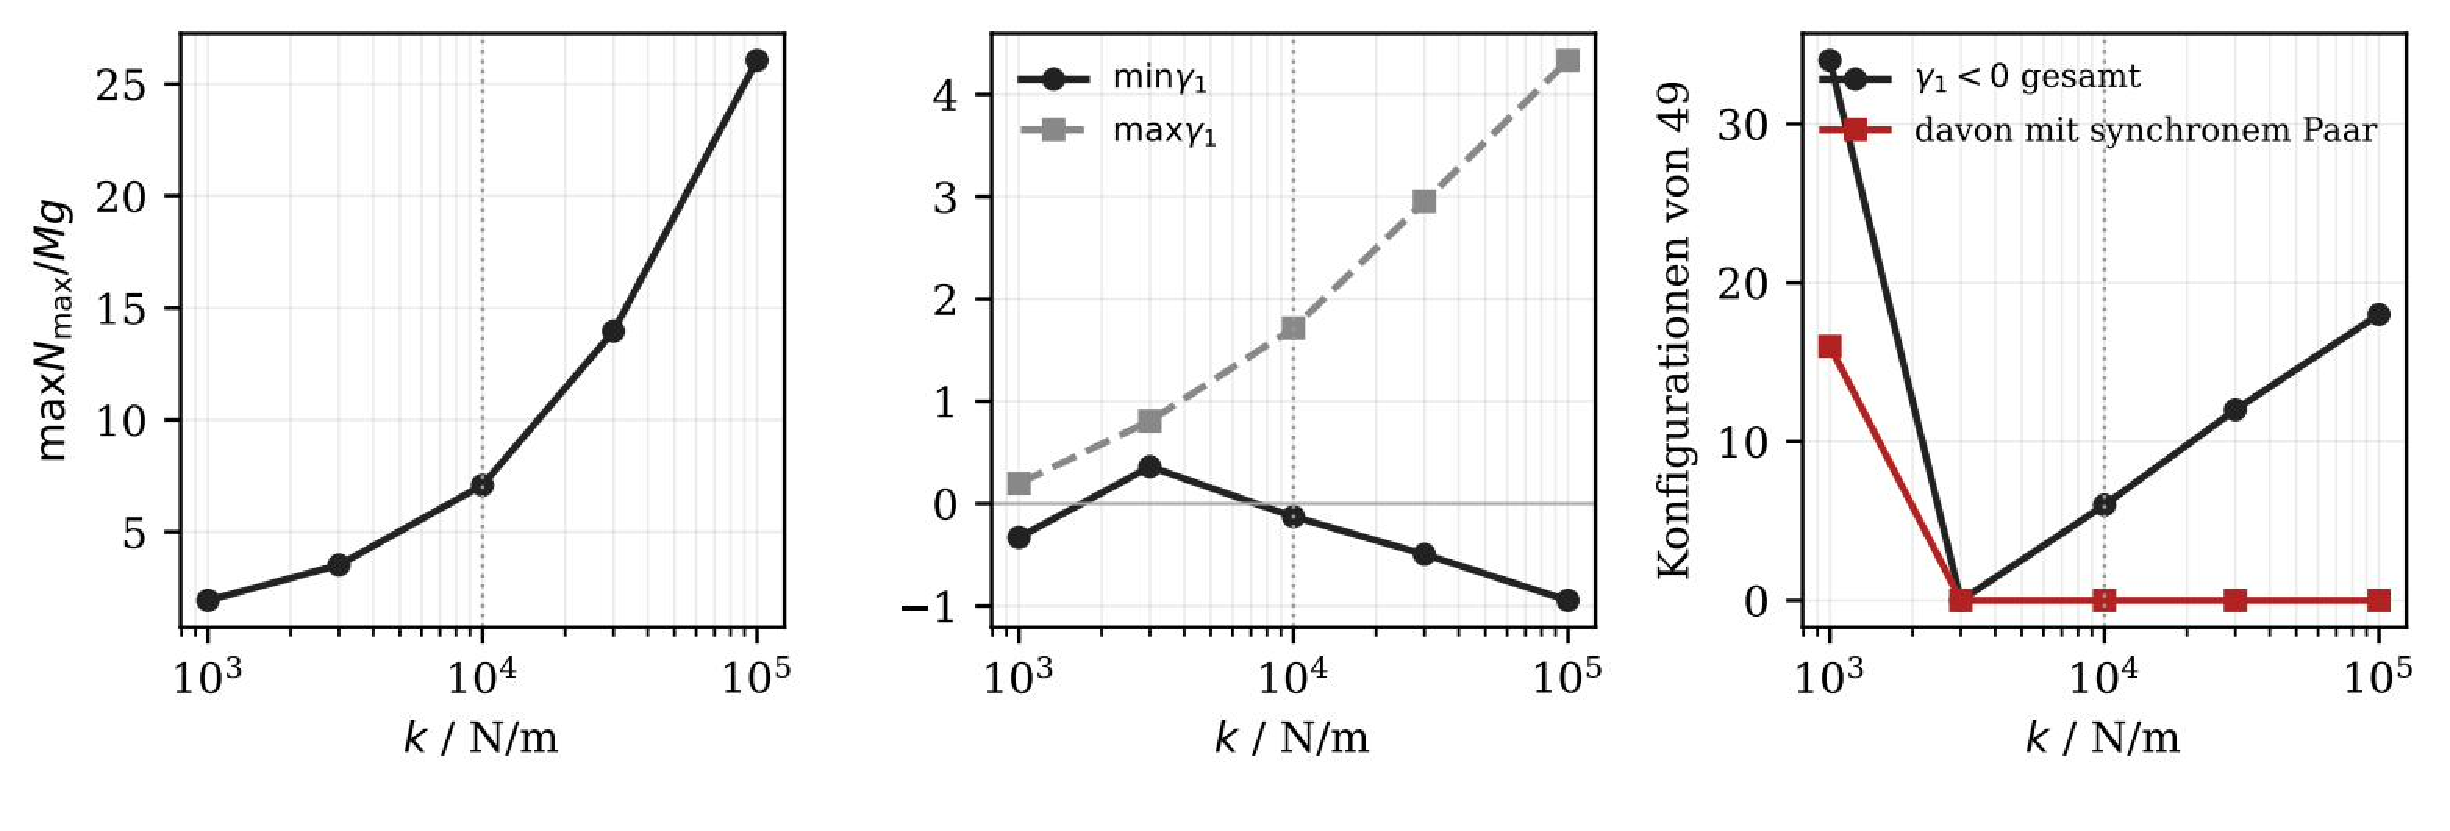
\includegraphics[width=\textwidth]{Plots/sens_k.pdf}
  \caption{Kennzahlen gegen die Kontaktsteifigkeit. Links die maximale
  Spitzenkraft, Mitte die Spannweite der Schiefe, rechts die Zahl der
  Konfigurationen mit negativer Schiefe und davon jene mit synchronem
  Modulpaar. Punktiert der Basisparametersatz.}
  \label{fig:sens-k}
\end{figure}

Vier Befunde, in der Reihenfolge ihrer Bedeutung für die Auslegung.

\paragraph{Die Vorzeichenregel hat einen Gültigkeitsbereich.}
Für $k \geq 3\cdot10^{3}\,\mathrm{N/m}$, also $3f/f_n \leq 2{,}8$, tritt
negative Schiefe in keiner Konfiguration mit gleichphasigem Modulpaar
auf; die Vorhersage aus Abschnitt~\ref{sec:vorhersage-schiefe} hält über
anderthalb Dekaden. Bei $k = 10^{3}\,\mathrm{N/m}$ bricht sie: 16 der 34
Konfigurationen mit negativer Schiefe enthalten ein synchrones Paar. Der
Grund ist die Lage der Anregung zur Kontaktresonanz. Bei
$k = 10^{3}\,\mathrm{N/m}$ liegt $f_n = 6{,}2\,\mathrm{Hz}$ unterhalb
der Anregungsfrequenz; der Kontakt arbeitet im Isolationsbereich mit
einer Transmissibilität von rund $0{,}66$. Der Rahmen bewegt sich dann
weitgehend mit den inneren Massen mit, und der Kontakt überträgt nur
einen gedämpften, zu höheren Harmonischen hin zunehmend abgeflachten
Anteil der Trägheitskraft. Die Kontaktkraft variiert entsprechend wenig
--- $N_{\max}$ erreicht nur das $1{,}9$-fache der Basislinie ---, ihre
Schiefe bleibt klein, $|\gamma_1| \leq 0{,}33$, und deren Vorzeichen ist
nicht mehr an die Phasenpaarung gebunden. Im entgegengesetzten Grenzfall
des steifen Kontakts, $3f/f_n \to 0$, überträgt die Unterlage die
Trägheitskraft nahezu unverzögert, $N(t) \approx Mg - (M/3)\sum
\ddot{z}_{\mathrm{egg}}$, und dort hält die Regel. Die Vorzeichenregel
ist also keine Eigenschaft des Profils allein, sondern des Zusammenspiels
von Profil und Kontaktdynamik --- und sie gilt nur, wo der Kontakt die
Profilform überträgt statt sie zu filtern.

\paragraph{Die Spitzenkraft wächst steil mit der Steifigkeit.}
$\max N_{\max}/Mg$ steigt von $1{,}9$ bei $k = 10^{3}$ auf $26$ bei
$k = 10^{5}$, näherungsweise proportional zu $\sqrt{k}$. Die
Nennlastforderung aus Abschnitt~\ref{sec:auslegung-sim} ist damit an
$k$ gebunden: Ein Metallkontakt statt eines Elastomerpads verlangt eine
um eine Größenordnung höhere Nennlast --- bei
$k = 10^{5}\,\mathrm{N/m}$ rund $170\,\mathrm{N}$ --- und verliert
entsprechend Auflösung um $Mg$.

\paragraph{Nahe der Kontaktresonanz verschwindet die Struktur.}
Bei $k = 3\cdot10^{3}\,\mathrm{N/m}$ liegt $f_n$ mit $10{,}8\,\mathrm{Hz}$
fast auf der Anregungsfrequenz. Dort hebt der Kontakt in jeder der 49
Konfigurationen ab, negative Schiefe tritt nirgends auf, und die
Spannweite der Schiefe ist die kleinste der Serie. Die Resonanz
verwischt die Regime. Ein Aufbau, dessen Kontakteigenfrequenz nahe $f$
liegt, ist für die Fragestellung ungeeignet, unabhängig von seiner
sonstigen Qualität.

\paragraph{Steifer Kontakt schärft die Regime.}
Mit wachsendem $k$ wird die negative Schiefe ausgeprägter --- von
$-0{,}13$ bei $10^{4}$ auf $-0{,}95$ bei $10^{5}$ --- und die
liftoff-freie Insel um die triphasische Konfiguration größer. Das
Signal, das die Vorzeichenregel prüft, wird also mit der Steifigkeit
deutlicher. Der Preis ist die Spitzenkraft, und die Flanke: Bandbreite
und Abtastrate skalieren nach Abschnitt~\ref{sec:bandbreite} mit $f_n$.

\paragraph{Anhaltspunkte für ein Auslegungsfenster.}
Aus den vier Befunden ergeben sich Anhaltspunkte für ein Fenster in
$3f/f_n$ --- Anhaltspunkte, weil fünf Steifigkeiten auf einem
$7\times7$-Raster kein durchgehend abgesichertes Fenster in Steifigkeit,
Dämpfung und Phasenlage begründen. Oberhalb von etwa
$3$ ist der Kontakt zu weich: Die Anregung liegt über der
Kontaktresonanz, der Kontakt filtert die Profilform, wenig Liftoff,
Schiefe klein und ohne Vorzeichenbindung, Regel ungültig. Um $3f/f_n \approx 3$ liegt die
Resonanz, die alles verwischt. Unterhalb von etwa $1$ ist der Kontakt
steif: Regel robust, Signal deutlich, aber Spitzenkraft und Bandbreite
teuer. Der Basisparametersatz mit $3f/f_n = 1{,}5$ liegt im Fenster;
$k = 3\cdot10^{4}\,\mathrm{N/m}$ mit $3f/f_n = 0{,}88$ würde das
Vorzeichensignal vervierfachen und die Spitzenkraft verdoppeln. Diese
Abwägung ist vor der Wahl des Kontaktelements zu treffen, und sie ist
mit den Zahlen der Tabelle~\ref{tab:sens-k} treffbar.

\subsection*{Dämpfung}

Die Dämpfung wurde bei festem $k = 10^{4}\,\mathrm{N/m}$ an den vier
Regimepunkten der Tabelle~\ref{tab:flanke} variiert, nicht über ein
Raster; die Aussagen sind entsprechend punktuell.

\begin{table}[htbp]
  \centering
  \begin{tabular}{rr|rr|rr|rr}
    \hline
    & & \multicolumn{2}{c|}{synchron} & \multicolumn{2}{c|}{Zweiergruppe} & \multicolumn{2}{c}{dephasiert} \\
    $\zeta$ & $c$ / N\,s/m & $\gamma_1$ & $N_{\max}/Mg$ & $\gamma_1$ & $\lambda$ / \% & $\gamma_1$ & $\lambda$ / \% \\
    \hline
    0{,}02 &  3{,}2 & $+2{,}91$ & 13{,}0 & $+1{,}66$ & 73{,}9 & $+0{,}01$ & 9{,}4 \\
    0{,}05 &  8{,}1 & $+2{,}99$ & 15{,}9 & $+1{,}66$ & 74{,}4 & $-0{,}08$ & 0{,}0 \\
    0{,}10 & 16{,}1 & $+1{,}71$ &  6{,}5 & $+1{,}66$ & 75{,}1 & $-0{,}28$ & 0{,}0 \\
    0{,}20 & 32{,}2 & $+1{,}77$ &  6{,}5 & $-0{,}07$ & 34{,}5 & $-0{,}63$ & 0{,}0 \\
    0{,}40 & 64{,}5 & $+2{,}05$ &  7{,}5 & $+0{,}08$ & 25{,}4 & $-0{,}74$ & 0{,}0 \\
    \hline
  \end{tabular}
  \caption{Dämpfungssensitivität an drei Regimepunkten,
  $k = 10^{4}\,\mathrm{N/m}$. Die vierte Konfiguration (stark
  intermittent) verhält sich über den gesamten Bereich wie die
  synchrone und ist nicht aufgeführt.}
  \label{tab:sens-zeta}
\end{table}

Drei Befunde.

\paragraph{Das Vorzeichensignal wächst mit der Dämpfung.} In der
dephasierten Konfiguration fällt $\gamma_1$ monoton von $-0{,}08$ bei
$\zeta = 0{,}05$ auf $-0{,}74$ bei $\zeta = 0{,}40$. Bei sehr schwacher
Dämpfung, $\zeta = 0{,}02$, verliert dieselbe Konfiguration den
Dauerkontakt --- $\lambda = 9{,}4\,\%$ --- und die Schiefe geht auf
null. Die liftoff-freie Insel um die triphasische Konfiguration setzt
also eine Mindestdämpfung voraus; ein sehr schwach gedämpfter Kontakt
prellt sie weg.

\paragraph{Die Vorzeichenregel hat auch in der Dämpfung einen
Gültigkeitsbereich.} Bei $\zeta = 0{,}20$ zeigt die Zweiergruppe
$\gamma_1 = -0{,}07$: eine Konfiguration mit gleichphasigem Modulpaar
und schwach negativer Schiefe, im Widerspruch zur Regel. Die Verletzung
ist klein, aber sie ist eine. An den vier geprüften Punkten hält die
Regel für $\zeta \lesssim 0{,}1$ und darüber nicht; für sämtliche
Phasenlagen ist sie damit nicht belegt. Zusammen mit dem Befund zur
Steifigkeit gilt: Die Vorhersage aus
Abschnitt~\ref{sec:vorhersage-schiefe} ist nach den Stichproben an
einen Bereich in $(k, \zeta)$ gebunden, dessen Grenzen vor der Kampagne
durch Ausschwingversuch und eine dichtere Abtastung zu bestimmen sind.

\paragraph{Die Spitzenkraft hängt nicht monoton von der Dämpfung ab.}
Im synchronen Fall erreicht $N_{\max}$ bei $\zeta = 0{,}05$ das
$15{,}9$-fache der Basislinie, rund $101\,\mathrm{N}$ --- mehr als bei
schwächerer wie bei stärkerer Dämpfung. Die Nennlastforderung aus
Abschnitt~\ref{sec:auslegung-sim} ist daher am schwach gedämpften
Fall zu bemessen: Eine Dose mit $10\,\mathrm{kg}$ Nennlast reicht bei
$\zeta = 0{,}10$, wird bei $\zeta = 0{,}05$ überschritten. Da $\zeta$
eines Elastomerpads vor der Messung nur ungefähr bekannt ist, ist die
Reserve entsprechend zu wählen.

\section{Was dieses Kapitel nicht belegt}

\begin{itemize}
  \item \textbf{Das Kontaktmodell ist nicht validiert.} Der Kontakt wird
        als linear-elastisch mit viskoser Dämpfung behandelt, ohne
        Hertz'sche Nichtlinearität, Rauheit oder Stoßverluste. Die Frage,
        die das Experiment behandelt, ist gerade, ob die hier gefundene
        Phasenabhängigkeit den Übergang zum realen Kontakt übersteht.
        Übereinstimmung zwischen Messung und Simulation ist nicht das
        Erfolgskriterium; das Überleben der qualitativen Struktur ist es.
  \item \textbf{Numerische Residuen sind keine Nachweisgrenzen.} Der
        Boden von $0{,}2\,\mathrm{ppm}$ aus
        Abschnitt~\ref{sec:track1-sim} ist eine Eigenschaft des
        Integrators. Er trägt keine Information über die erreichbare
        Messauflösung. Die Schwelle $\varepsilon_{\mathrm{phys}}$ wird
        empirisch aus der Wiederholpräzision der Referenz bestimmt und
        aus nichts sonst.
  \item \textbf{Die Wertebereiche sind keine Vorhersagen.}
        Tabelle~\ref{tab:functional-range} gibt an, wie weit sich die
        Funktionale im Modell bewegen. Sie gibt nicht an, wie weit sie
        sich in der Apparatur bewegen werden.
\end{itemize}

\section{Berichtsformat der Messkampagne}

Das Kapitel, das die Messergebnisse berichtet, ist zum jetzigen Zeitpunkt
bewusst leer. Sein Format wird hier festgelegt, bevor Daten vorliegen,
und nach der Erhebung nicht mehr geändert:

\begin{enumerate}
  \item Wiederholpräzision der Referenz:
        $\hat{\sigma}_{\mathrm{ref}}$ je Funktional und die daraus
        folgende Schwelle $\varepsilon_{\mathrm{phys}}$.
  \item Ergebnis der Spur~1: Kontrollgröße mit Konfidenzintervall,
        getrennt berichtet für Konfigurationen mit niedrigem und mit
        hohem Liftoff-Anteil, sowie die daraus folgende Schranke für die
        systematische Verschiebung.
  \item Ergebnis der Spur~2: die vier Funktionale über die gemessenen
        Konfigurationen, mit Bootstrap-Intervallen.
  \item Klassifikation des Ausgangs nach
        Abschnitt~\ref{sec:decision-class}, mit den ausgeschlossenen
        Läufen und dem angewandten Ausschlusskriterium.
  \item Etwaige Abweichungen von diesem Format, einzeln aufgeführt und
        begründet.
\end{enumerate}

Ein Nullergebnis wird im selben Format und in derselben Ausführlichkeit
berichtet wie ein positives.

% ------------------------------------------------------

\chapter{Artefaktanalyse}
\label{chap:artefakt}

\section{Überblick}

Das Erkennen und Beherrschen experimenteller Artefakte ist eine zentrale
Voraussetzung für die Auslegung kleiner Signalabweichungen. Da die
erwartete Signalgröße mit der Messunsicherheit vergleichbar ist, können
bereits geringe unkontrollierte Effekte scheinbare Unterschiede zwischen
Systemzuständen erzeugen.

Dieses Kapitel benennt, klassifiziert und bewertet systematisch mögliche
Artefaktquellen. Sie sind gegen zwei verschiedene Zielsignaturen zu
prüfen, und die Prüfungen sind nicht austauschbar:

\begin{itemize}
\item Artefakte, die eine Abweichung der Kontrollgröße von null
      erzeugen. Da diese Größe erhaltungsgarantiert null ist, ist jede
      solche Abweichung definitionsgemäß ein Artefakt; die Frage lautet
      nur, welches.
\item Artefakte, die eine scheinbare Abhängigkeit der
      Wellenformfunktionale von der Phasenkonfiguration erzeugen. Diese
      sind schwerer zu erkennen, da hier kein bekannter Sollwert
      vorliegt.
\end{itemize}

Die zweite Klasse ist die kritische. Ein Artefakt, das mit der
Phasenlage der Aktuierung korreliert --- etwa elektromagnetische
Einkopplung oder ein phasengebundener Synchronisationsversatz ---
erzeugt genau die Signatur, die auch ein echter Befund erzeugen würde.

\section{Definition von Artefakten}

Als Artefakt gilt in dieser Arbeit jeder Beitrag zum gemessenen Signal,
der nicht unmittelbar mit der beabsichtigten zustandsabhängigen
Änderung des Systems zusammenhängt, sondern aus dem Messvorgang, aus
Umgebungseinflüssen oder aus unbeabsichtigtem Systemverhalten entsteht.

Artefakte können Signale erzeugen, die

\begin{itemize}
\item zeitabhängig,
\item zustandsabhängig,
\item oder statistisch strukturiert sind,
\end{itemize}

und die daher ohne gezielte Analyse von der Zielgröße nicht
unterscheidbar sein können.

\section{Klassifikation der Artefaktquellen}

Mögliche Artefaktquellen werden in die folgenden Kategorien gegliedert.

\subsection{Mechanische Artefakte}

\begin{itemize}
\item unbeabsichtigte Kopplung zwischen innerer Bewegung und äußerer
      Struktur,
\item Asymmetrien der Massenverteilung,
\item Verformung tragender Bauteile,
\item Reibung und Stick-Slip-Effekte,
\item Lose oder Spiel in mechanischen Verbindungen.
\end{itemize}

\subsection{Sensorbedingte Artefakte}

\begin{itemize}
\item Sensordrift und instabile Nulllage,
\item nichtlineares Sensorverhalten,
\item Hysterese,
\item Querempfindlichkeit gegenüber Temperatur oder Erschütterung,
\item begrenzte Auflösung und Quantisierungseffekte.
\end{itemize}

\subsection{Umgebungsbedingte Artefakte}

\begin{itemize}
\item Temperaturschwankungen,
\item Umgebungserschütterungen,
\item Luftströmungen oder Druckänderungen,
\item elektromagnetische Störeinflüsse.
\end{itemize}

\subsection{Artefakte aus Steuerung und Aktuierung}

\begin{itemize}
\item Ungenauigkeiten im Zeitverhalten der Aktuierung,
\item Phasenjitter,
\item Schwankungen der Spannungsversorgung,
\item Kopplung zwischen Steuerelektronik und Messsystem.
\end{itemize}

\subsection{Artefakte der Datenerfassung}

\begin{itemize}
\item Abtastjitter,
\item Synchronisationsfehler,
\item Signalbegrenzung oder Sättigung,
\item Grenzen der numerischen Genauigkeit.
\end{itemize}

\section{Wirkmechanismen}

Jeder Artefaktquelle ist ein Mechanismus zugeordnet, über den sie das
gemessene Signal beeinflussen kann. Dazu zählen:

\begin{itemize}
\item die Erzeugung eines unmittelbaren Kraftbeitrags,
\item die Veränderung des Kraftflusses,
\item das Einbringen einer zeitabhängigen Verschiebung,
\item die Kopplung zwischen innerer Dynamik und Messschnittstelle,
\item die Verzerrung des aufgezeichneten Signals.
\end{itemize}

Das Verständnis dieser Mechanismen ist notwendig, um zu beurteilen, ob
ein beobachtetes Signal plausibel aus einem Artefakt stammen kann.

\section{Unterscheidungskriterien}

Zur Abgrenzung einer echten zustandsabhängigen Änderung gegen ein
Artefakt werden die folgenden Kriterien herangezogen:

\begin{itemize}
\item die Abhängigkeit von äußeren Größen wie der Temperatur,
\item die Empfindlichkeit gegenüber kleinen Änderungen der
      Aufbaukonfiguration,
\item die Korrelation mit Hilfssignalen, etwa der Erschütterungsmessung,
\item der Bestand über wiederholte Läufe hinweg,
\item Symmetrie oder Asymmetrie gegenüber einer Zustandsumkehr.
\end{itemize}

Ein beobachteter Effekt, der stark mit unkontrollierten Parametern
variiert, ist mit höherer Wahrscheinlichkeit artefaktbedingt.

\section{Kontrollversuche}

Eigene Kontrollversuche dienen dazu, Artefaktbeiträge zu isolieren und
zu bewerten. Beispiele sind:

\begin{itemize}
\item der Betrieb des Systems ohne innere Aktuierung,
\item symmetrische Konfigurationen, bei denen kein Nettounterschied zu
      erwarten ist,
\item die Variation der Umgebungsbedingungen innerhalb kontrollierter
      Grenzen,
\item die Änderung der Einspannbedingungen,
\item der Austausch von Komponenten, etwa des Sensors.
\end{itemize}

Ziel der Kontrollversuche ist nicht die Bestätigung eines Effekts,
sondern die Prüfung alternativer Erklärungen.

\section{Empfindlichkeitsanalyse}

Die Empfindlichkeit der Messgrößen gegenüber Änderungen von
Systemparametern wird bewertet, indem ausgewählte Parameter systematisch
verändert und die resultierende Änderung der Zielfunktionale
$\gamma_1$, $\lambda$, $A$ und $N_{\min}$ beobachtet wird. Die
Kontrollgröße wird dabei mitgeführt: Verändert sie sich mit einem
Parameter, der sie nach Gleichung~\eqref{eq:baseline-ch3} nicht
verändern kann, ist der betreffende Parameter selbst eine Artefaktquelle.

Zu den Parametern können gehören:

\begin{itemize}
\item die Anregungsamplitude,
\item die Phasenbeziehungen,
\item die Frequenz,
\item die Länge des Messfensters,
\item die Umgebungsbedingungen.
\end{itemize}

Eine starke Abhängigkeit von unbeabsichtigten Parametern kann auf ein
Überwiegen von Artefakten hindeuten.

\section{Residualanalyse}

Die durch $C(x,t)$ dargestellten Residualbeiträge werden analysiert,
indem gemessene Daten mit dem unter vereinfachten Annahmen erwarteten
Verhalten verglichen werden. Abweichungen, die das Primärmodell nicht
erklärt, werden Residualeffekten zugeordnet und weiter untersucht.

Die Residualanalyse umfasst:

\begin{itemize}
\item den Vergleich von gemessener und erwarteter Signalstruktur,
\item das Erkennen systematischer Muster in den Residuen,
\item die Bewertung der Korrelation mit Hilfsmessungen.
\end{itemize}

\section{Betrachtung des ungünstigsten Falls}

Um Überinterpretation zu vermeiden, wird ein Vorgehen nach dem
ungünstigsten Fall gewählt. Für jeden beobachteten Effekt wird gefragt:

\begin{quote}
Lässt sich das beobachtete Signal vollständig durch bekannte oder
plausible Artefaktmechanismen erklären?
\end{quote}

Nur wenn keine plausible Artefakterklärung mit den Daten vereinbar
bleibt, gilt das Ergebnis als Kandidat für eine weitergehende Auslegung.

\section{Dokumentation und Nachvollziehbarkeit}

Alle erkannten Artefaktquellen, Kontrollversuche und Analyseschritte
werden ausführlich dokumentiert. Dazu gehören:

\begin{itemize}
\item die Beschreibung der Prüfbedingungen,
\item die Parametereinstellungen,
\item die beobachteten Effekte,
\item die Schlussfolgerungen zur Relevanz des jeweiligen Artefakts.
\end{itemize}

Diese Dokumentation sichert, dass der Bewertungsvorgang durchsichtig und
reproduzierbar bleibt.

\section{Grenzen der Artefaktanalyse}

Eine vollständige Beseitigung aller Artefakte ist nicht erreichbar. Ziel
ist daher nicht der Nachweis ihrer Abwesenheit, sondern die Verringerung
ihres Einflusses und die Beurteilung ihrer Plausibilität im Verhältnis
zum beobachteten Signal.

Unerkannte oder zusammenwirkende Artefakteffekte können weiterhin
vorliegen und sind in der abschließenden Auslegung zu berücksichtigen.

\section{Zwischenfazit}

Die Artefaktanalyse ist integraler Bestandteil der experimentellen
Methodik. Sie liefert ein strukturiertes Vorgehen, um alternative
Erklärungen beobachteter Signalabweichungen zu benennen und zu bewerten.

Der Rahmen betont kritische Bewertung, kontrollierte Prüfung und
zurückhaltende Auslegung, um das Risiko falsch-positiver Schlüsse gering
zu halten.

% ------------------------------------------------------

\chapter{Diskussion}
\label{chap:diskussion}

\section{Überblick}

Dieses Kapitel bewertet, was die Arbeit zum gegenwärtigen Stand
festgestellt hat und was sie ausdrücklich nicht festgestellt hat. Es
liegen keine Messdaten vor; die Erörterung bezieht sich daher auf den
Rahmen selbst und auf die Simulationsstudie nach
Kapitel~\ref{chap:simulation}.

Das ist keine Einschränkung des Diskussionsgegenstands, sondern seine
Bestimmung. Ein prä-experimenteller Rahmen wird nicht danach beurteilt,
welche Ergebnisse er hervorgebracht hat, sondern danach, ob er
Ergebnisse hervorbringen könnte, die belastbar sind --- und ob er die
Bedingungen benennt, unter denen sie es nicht wären.

\section{Was die Simulationsstudie zeigt}
\label{sec:sim-zeigt}

Zwei Befunde liegen vor. Beide sind Modellaussagen und keine Messungen.

\vspace{0.5em}

\textbf{Das Fenstermittel trägt bei intermittierendem Kontakt einen
Randterm.} Über die $361$ Konfigurationen des Rasters gewinnt die Kette
die erhaltene Basislinie bei Dauerkontakt auf $0{,}2\,\mathrm{ppm}$
zurück; im Archivlauf erreichte das Residuum bei Liftoff-Anteilen
oberhalb von $50\,\%$ bis $0{,}68\,\%$. Der Schwerpunktsatz lässt bei
hohem Liftoff keine Ausnahme zu, legt aber für jedes endliche Fenster
einen Randterm fest: die Änderung der Schwerpunktsgeschwindigkeit,
bezogen auf $g$ und Fensterlänge (Gleichung~\eqref{eq:randterm}). Das
Residuum fällt mit $T_w^{-0{,}945}$, also praktisch mit $T_w^{-1}$,
während ein Integrationsfehler von der Fensterlänge unabhängig wäre; der
Quadraturanteil bleibt unter $0{,}01\,\%$. Der Höchstwert des Archivs war
Einschwingen; bei aperiodischer Bewegung bleibt der Randterm im
$10$-s-Fenster bis $0{,}37\,\%$.

Der methodisch erhebliche Teil ist nicht der Wert, sondern die Art seines
Zustandekommens: Der Befund wurde durch eine Größe erzeugt, deren
richtige Antwort vorab bekannt war. Ohne diese Konstruktion wäre der
Randterm nicht als solcher erkennbar gewesen, sondern hätte
als konfigurationsabhängiger Effekt erscheinen können. Genau das ist in
einer früheren Phase dieses Projekts geschehen.

\vspace{0.5em}

\textbf{Die Zielgrößen sind im Modell nicht entartet.} Die
Wellenformfunktionale überstreichen den Raum der Phasenkonfigurationen um
Faktoren, während das Zeitmittel innerhalb von $0{,}07\,\%$ festliegt.
Die Spitzenkontaktkraft erreicht das Achtfache der Basislinie. Damit ist
die erforderliche Messauflösung bezifferbar, und die Frage nach einer
Phasenabhängigkeit ist im Modell nicht trivial beantwortet.

\section{Was die Simulationsstudie nicht zeigt}

Die Grenzen dieser Befunde sind schärfer als ihre Aussage.

\begin{itemize}
\item \textbf{Das Kontaktmodell ist nicht validiert.} Es behandelt den
      Kontakt als linear-elastisch mit viskoser Dämpfung, ohne
      Hertz'sche Nichtlinearität, Rauheit oder Stoßverluste. Ob die im
      Modell gefundene Struktur den Übergang zum realen Kontakt
      übersteht, ist gerade die offene Frage.
\item \textbf{Das numerische Residuum ist keine Nachweisgrenze.} Der
      Boden von $0{,}2\,\mathrm{ppm}$ bei Dauerkontakt ist eine
      Eigenschaft des Integrators, der Anstieg bei Intermittenz eine
      Eigenschaft der gewählten Fensterlänge. Beides sagt nichts über
      die erreichbare Messauflösung.
\item \textbf{Die Parametersätze sind nicht abgeglichen.} Die Simulation
      arbeitet mit $10\,\mathrm{Hz}$ und einem Halteanteil von $0{,}65$,
      während für die Apparatur $2{,}2\,\mathrm{Hz}$ und $0{,}80$ als
      Auslegungswerte geführt werden. Bis dieser Abgleich vorliegt,
      lassen sich die Zahlenwerte des Kapitels~\ref{chap:simulation}
      nicht auf die Apparatur übertragen.
\end{itemize}

\section{Die Kontrollgröße als Instrument --- und ihre Grenze}
\label{sec:kontrollgrenze}

Der zentrale methodische Zug dieser Arbeit ist die Verwendung einer
erhaltungsgarantierten Nullgröße als In-situ-Kontrolle. Seine Stärke ist
unmittelbar: Er liefert eine Nullreferenz ohne Zweitapparatur, ohne
Referenznormal und ohne Modellannahme, und er misst das
Falsch-Positiv-Verhalten der vollständigen Auswertekette gegen eine
bekannte Antwort.

Seine Grenze ist ebenso unmittelbar und wird hier ausdrücklich benannt,
weil sie die Reichweite des gesamten Rahmens bestimmt.

\vspace{0.5em}

\textbf{Die Kontrolle deckt nicht ab, was sie zu decken scheint.} Der
Nachweis, dass die Kette eine erhaltungsgarantierte Nullgröße als null
wiedergewinnt, ist eine Aussage über das \emph{erste Moment}. Die
Zielgrößen sind Funktionale der Wellenform. Aus der Bestätigung der
einen folgt die Verlässlichkeit der anderen nicht.

Konkret bestehen mindestens drei Artefaktklassen die Kontrolle und
verfälschen dennoch das Ergebnis:

\begin{itemize}
    \item \textbf{Phasenkorrelierte Einkopplung.} Ein Störsignal, das
    mit dem Aktuierungstakt korreliert --- elektromagnetische
    Einkopplung, ein phasengebundener Synchronisationsversatz ---
    verändert die Wellenform, kann sich aber über den Zyklus zu null
    mitteln. Die Kontrollgröße bleibt dann unauffällig, während
    $\gamma_1$, $\lambda$ und $A$ systematisch verfälscht sind. Dies ist
    die kritische Klasse.
    \item \textbf{Symmetrischer Kettenfehler.} Ein Fehler, der beide
    Zustände gleichermaßen trifft, hebt sich in der Differenz auf. Die
    Kontrolle besteht, obwohl die Kette einen erheblichen systematischen
    Fehler trägt.
    \item \textbf{Amplitudenabhängige Kennlinie.} Bei zyklischer
    Trennung durchläuft die Eingangskraft den Bereich von null bis zum
    Vielfachen der Basislinie. Eine über diesen Bereich nicht konstante
    Übertragung verzerrt die Wellenform, ohne das Zeitmittel zu
    verschieben.
\end{itemize}

Die Kontrolle ist damit eine \emph{notwendige}, keine hinreichende
Bedingung. Sie schließt eine Fehlerklasse sicher aus --- diejenige, die
in diesem Projekt tatsächlich zu einem zurückgezogenen Befund geführt hat
--- und lässt andere offen.

\vspace{0.5em}

\textbf{Was daraus folgt.} Die verbleibenden Klassen sind nicht
statistisch, sondern nur durch Versuchsanordnung zu behandeln. Drei
Maßnahmen sind dafür vorgesehen und in Kapitel~\ref{chap:artefakt}
ausgeführt:

\begin{itemize}
    \item Leerläufe mit bestromter, aber blockierter Aktuierung. Sie
    trennen elektromagnetische Einkopplung von mechanischer Wirkung,
    weil die elektrische Anregung unverändert bleibt und die mechanische
    entfällt. Dies ist der wichtigste Einzelversuch des gesamten
    Protokolls.
    \item Umkehr der Phasenreihenfolge. Eine echte Abhängigkeit von der
    Phasenkonfiguration ist gegenüber der Messreihenfolge invariant, ein
    taktgebundenes Artefakt nicht notwendig.
    \item Statische Kennlinienaufnahme über den gesamten Kraftbereich
    bis zum Achtfachen der Basislinie, statt nur um den Arbeitspunkt.
\end{itemize}

\section{Bezug zur Artefaktanalyse}

Die Auslegung der Ergebnisse ist von der systematischen Artefaktanalyse
nicht zu trennen. Nach der Unterscheidung in
Abschnitt~\ref{sec:kontrollgrenze} gilt für die beiden Größenklassen
Verschiedenes:

Bei der \textbf{Kontrollgröße} ist die Zuordnung eindeutig. Ihr wahrer
Wert ist null; jede statistisch belastbare Abweichung ist ein Artefakt,
und die Aufgabe der Analyse besteht allein darin, welches. Der
Artefaktkatalog dient hier der Eingrenzung, nicht der Entscheidung.

Bei den \textbf{Wellenformfunktionalen} liegt kein Sollwert vor. Hier
trägt die Analyse die Entscheidungslast, und ein beobachtetes Signal
gilt nur dann als Kandidat, wenn es

\begin{itemize}
    \item über unabhängige Läufe hinweg reproduzierbar ist,
    \item mit dem gesteuerten Systemzustand korreliert und nicht mit dem
    Aktuierungstakt,
    \item unter kontrollierter Parametervariation stabil bleibt,
    \item im Leerlauf mit blockierter Aktuierung verschwindet,
    \item keiner bekannten Artefaktsignatur entspricht.
\end{itemize}

Wird eine dieser Bedingungen verfehlt, erfolgt die Einstufung als
möglicher Artefaktbeitrag. Der vollständige Ausschluss aller
Artefaktbeiträge lässt sich nicht garantieren; die Aufgabe des Rahmens
ist die Verringerung der Fehldeutungswahrscheinlichkeit, nicht der
Beweis der Artefaktfreiheit.

\section{Grenzen der Auslegung}

Der Auslegungsrahmen ist ausdrücklich auf die Messebene beschränkt.

Jede beobachtete Abweichung kann stammen aus

\begin{itemize}
    \item ungeklärten Messartefakten,
    \item unvollständiger oder vereinfachter Systemmodellierung,
    \item Umgebungseinflüssen, die der Aufbau nicht vollständig erfasst,
    \item Residualbeiträgen, dargestellt durch den Term $C(x,t,\theta)$
    in Gleichung~\eqref{eq:zerlegung-voll}.
\end{itemize}

Ein Überschreiten der Schwelle $\varepsilon_{\mathrm{phys}}$ ist daher
eine notwendige, keine hinreichende Bedingung für die Behauptung einer
echten Phasenabhängigkeit. Ohne unabhängige Belege, die
artefaktbasierte Erklärungen ausschließen, wird keine kausale Auslegung
vorgenommen.

Umgekehrt gilt: Das Ausbleiben eines Befunds beweist nicht die
Abwesenheit einer Abhängigkeit. Eine obere Schranke ist nur dann
festgelegt, wenn das Intervall der Differenz nachweislich innerhalb der
Schwelle liegt; andernfalls ist der Ausgang unbestimmt, und es gibt
keine Schranke zu berichten. Und selbst ein nachgewiesenes
Nullergebnis ist nur so aussagekräftig wie die zugrunde liegende
Wiederholpräzision: Bei großem $\hat{\sigma}_{\mathrm{ref}}$ ist die
Schwelle weit, die Schranke schwach --- und muss als solche berichtet
werden, statt als Ausschluss.

\section{Unabhängigkeit und statistische Annahmen}

Die statistische Auswertung setzt voraus, dass die laufweisen Schätzwerte
näherungsweise unabhängig sind.

Verletzungen dieser Annahme können entstehen aus

\begin{itemize}
    \item thermischen Relaxationseffekten zwischen den Läufen,
    \item langsamen Driftvorgängen auf Zeitskalen, die mit der Messfolge
    vergleichbar sind,
    \item Gedächtniseffekten im mechanischen oder elektronischen System,
    insbesondere Setzvorgängen in der Einspannung.
\end{itemize}

Solche Effekte bringen Korrelationen ein, die das statistische
Standardmodell nicht erfasst, und verzerren die Schätzung der Streuung.
Da die Entscheidungsschwelle aus eben dieser Streuung abgeleitet wird,
wirkt sich eine unterschätzte Streuung unmittelbar auf die
Entscheidungsregel aus: Die Schwelle fällt zu niedrig aus, und die
Falsch-Positiv-Rate steigt über das nominelle Niveau.

Für die Wellenformfunktionale kommt hinzu, dass die Annahme
näherungsweiser Normalverteilung der laufweisen Werte nicht
selbstverständlich ist. Bei hohem Liftoff-Anteil ist die
Kontaktkraftverteilung bimodal, mit einer Masse bei null und einer in der
Kontaktphase; das dritte Moment reagiert dann empfindlich auf die
Fensterwahl. Aus diesem Grund werden Bootstrap-Intervalle über die Läufe
verwendet und keine normalverteilungsbasierten Intervalle. Auch der
Bootstrap setzt jedoch Austauschbarkeit der Läufe voraus, die durch
Neueinspannung zwischen Sitzungen verletzt sein kann.

\section{Einschränkungen}

Die vorliegende Arbeit unterliegt den folgenden Einschränkungen:

\begin{itemize}
    \item \textbf{Es liegen keine Messdaten vor.} Alle Zahlenwerte
    stammen aus Simulationen. Der Rahmen ist ausgelegt, nicht erprobt.
    \item \textbf{Die dynamische Kalibrierung bei intermittierendem
    Kontakt ist ungelöst.} Die statische Rückführbarkeit des
    Kraftsensors ist verfügbar; ihre Übertragung auf einen Kontakt, der
    zyklisch abhebt, ist nicht abgesichert. Das begrenzt die absolute
    Auslegung von $N_{\max}$ und $A$ unmittelbar.
    \item \textbf{Die Schwellen sind nicht beziffert.}
    $\varepsilon_{\mathrm{phys}}$ und $\varepsilon_{\perp}$ sind
    definiert, aber ihre Werte folgen erst aus der
    Wiederholmesskampagne. Bis dahin lässt sich ein Nullergebnis nicht
    formal von unzureichender Auflösung unterscheiden.
    \item \textbf{Die Kontrolle deckt nicht alle Fehlerklassen ab}, wie
    in Abschnitt~\ref{sec:kontrollgrenze} ausgeführt.
    \item \textbf{Endliche Auflösung und begrenzte Laufzahl} begrenzen
    die Teststärke.
\end{itemize}

Diese Einschränkungen begrenzen sowohl die Empfindlichkeit des geplanten
Versuchs als auch die Tragfähigkeit jedes daraus abgeleiteten Schlusses.

\section{Alternative Erklärungen}

Auch bei einem statistisch belastbaren und reproduzierbaren Befund sind
alternative Erklärungen zu prüfen. Plausible Quellen sind:

\begin{itemize}
    \item unbeabsichtigte mechanische Kopplung innerhalb des Systems,
    \item Asymmetrien im konstruktiven Aufbau,
    \item eine über den Kraftbereich nicht konstante Übertragung der
    Messkette,
    \item Wechselwirkung zwischen Aktuierungssignalen und
    Sensorelektronik,
    \item das Zusammenwirken mehrerer kleiner Artefaktbeiträge, von denen
    keiner für sich auffällig wäre.
\end{itemize}

Die letzte Möglichkeit ist die am schwersten auszuschließende. Der Rahmen
bevorzugt keine bestimmte Erklärung, verlangt aber den Ausschluss
artefaktbasierter Auslegungen, bevor eine weitergehende Deutung erwogen
wird.

\section{Übertragbarkeit}

Der dargestellte Zugang ist nicht auf das hier untersuchte System
beschränkt. Übertragbar ist insbesondere das konstruktive Prinzip: Wo
eine Erhaltungsgröße eine Messgröße auf einen bekannten Wert festlegt,
lässt sich diese Größe als In-situ-Kontrolle der Auswertekette verwenden,
statt sie als uninteressant zu übergehen.

Die Voraussetzungen dafür sind eng: Es muss eine Größe geben, deren
wahrer Wert theoretisch festliegt, die mit demselben Aufbau und derselben
Kette erfasst wird wie die Zielgröße, und die von den zu prüfenden
Konfigurationsänderungen unberührt bleibt. Wo diese drei Bedingungen
zutreffen, ist der Zugang anwendbar --- etwa bei Experimenten mit
kleinen Signalgrößen im Verhältnis zu Rauschen und Drift, komplexer
Systemdynamik, begrenzter Beobachtbarkeit innerer Zustände und hoher
Empfindlichkeit gegenüber Messartefakten.

Nicht übertragbar ist die Annahme, eine bestandene Kontrolle qualifiziere
die Kette für beliebige Zielgrößen. Die Kontrolle gilt für die Klasse von
Größen, der sie selbst angehört.


% ------------------------------------------------------

\chapter{Fazit}
\label{chap:fazit}

\section{Zusammenfassung der Arbeit}

Die Arbeit hat einen strukturierten Messrahmen für die Untersuchung
kleiner, zustandsabhängiger Abweichungen in Kraftsignalen mechanisch
gekoppelter Systeme entwickelt und angewandt.

Der Rahmen beruht auf:

\begin{itemize}
\item der ausdrücklichen Trennung von Systemdynamik und Messvorgang,
\item der formalen Unterscheidung von Drift, erhaltener Basislinie und
      Wellenformobservablen,
\item der Aufnahme von Residualbeiträgen,
\item vorab festgelegten statistischen Entscheidungskriterien,
\item einer systematischen Artefaktanalyse.
\end{itemize}

Ein Versuchsaufbau wurde entworfen, der kontrollierte Zustandsübergänge
und reproduzierbare Messungen unter definierten Randbedingungen
ermöglichen soll. Er ist zum Stand dieser Arbeit nicht ausgeführt. Die
Arbeit ist prä-experimentell: Sie legt die Kriterien fest, bevor Daten
vorliegen, und macht sie damit der nachträglichen Anpassung
unzugänglich.

\section{Wesentliche Befunde}
\label{sec:befunde}

Zum Stand dieser Arbeit liegen keine Messdaten vor. Die Befunde stammen
aus der Simulationsstudie nach Kapitel~\ref{chap:simulation} und sind
Modellaussagen. Sechs davon binden die Auslegung des Experiments.

\paragraph{Die Kontrollgröße hat einen Fenstereffekt sichtbar
gemacht.} Das Basislinienresiduum liegt bei Dauerkontakt bei
$0{,}2\,\mathrm{ppm}$. Größere Werte sind der Randterm des
Auswertefensters, die Impulsänderung des Schwerpunkts über das Fenster.
Er entsteht bei unvollständigem Einschwingen, bei Fenstern ohne ganze
Orbitperioden und bei aperiodischer Bewegung und fällt mit der
Fensterlänge; die Integration trägt unter $0{,}01\,\%$ bei. Da der
Liftoff-Anteil von der Phasenlage abhängt, erschien dieser Randterm in
einer früheren Projektphase als phasenabhängiger Effekt. Die Größe mit bekannter Antwort hat ihn als Artefakt
ausgewiesen.

\paragraph{Die Wellenformfunktionale sind nicht entartet, aber auch
nicht unabhängig.} Sie variieren über den Phasenraum um Faktoren,
während das Zeitmittel innerhalb von $0{,}07\,\%$ festliegt. Schiefe,
Liftoff-Anteil und Asymmetrieverhältnis korrelieren jedoch mit
$r \geq 0{,}93$; nur die minimale Kontaktkraft trägt eigenständige
Information.

\paragraph{Das Vorzeichen der Schiefe ist eine prüfbare Vorhersage.}
Negative Schiefe tritt nur auf, wenn kein
Modulpaar gleichphasig läuft. Die Regel hält in den geprüften
Stichproben für $3f/f_n \lesssim 2{,}8$ und $\zeta \lesssim 0{,}1$ und
bricht, sobald der Kontakt die Profilform filtert statt sie zu
übertragen. Sie ist mit drei Messungen prüfbar und benötigt keine
Nachweisschwelle.

\paragraph{Die Profilasymmetrie ist die Quelle der Phasenabhängigkeit.}
Mit sinusförmigem Antrieb kollabiert die Phasenkarte auf die
resultierende Amplitude $R$, negative Schiefe tritt nirgends auf, und
das Dreimodulsystem wird einem einzelnen Schwingerreger äquivalent. Für
den Aufbau ist ein Antrieb mit asymmetrischem Profil zwingend; Exzenter
und Kurbel bei konstanter Drehzahl scheiden aus.

\paragraph{Die Kontaktsteifigkeit gibt Anhaltspunkte für ein
Auslegungsfenster.} Zu weich filtert der Kontakt die Profilform, nahe
der Resonanz verwischen die Regime, zu steif wachsen Spitzenkraft und
Bandbreite. Der Basisparametersatz mit $3f/f_n = 1{,}5$ liegt nach den
Stichproben im Fenster; abgesichert ist es nicht.

\paragraph{Drei Zahlen binden die Messtechnik.} Die Nennlast ist am
Spitzenwert zu bemessen: $20\,\mathrm{kg}$ bei ungemessener Dämpfung,
$10\,\mathrm{kg}$ erst nach nachgewiesenem $\zeta \geq 0{,}1$, bei
steifem Kontakt entsprechend mehr. Bandbreite und Abtastrate folgen der
Kontakteigenfrequenz, $B \geq 10\,f_n$ und $f_s \geq 10\,B$. Die
Fensterlänge ist durch Konvergenznachweis zu bestimmen, nicht
anzunehmen.

Die Messkampagne selbst endet nach
Abschnitt~\ref{sec:decision-class} in genau einem von vier Zuständen:
Apparaturfehler, unbestimmt, nachgewiesenes Nullergebnis mit oberer
Schranke, oder nachgewiesene Abhängigkeit ohne Mechanismusbehauptung.
Der zweite ist ein bezifferbares Präzisionsdefizit, die übrigen drei
sind vollständige Ausgänge.

\section{Methodischer Beitrag}

Der wesentliche Beitrag dieser Arbeit ist methodisch. Die einzelnen
Elemente sind in Abschnitt~\ref{sec:beitrag} aufgeführt; hervorzuheben
ist der konstruktive Kern:

Eine Größe, die ein Erhaltungssatz auf einen bekannten Wert festlegt,
wird nicht als uninteressant übergangen, sondern als Prüfmittel gegen die
eigene Auswertekette verwendet. Damit entsteht eine Nullreferenz ohne
Zweitapparatur, und die Zielgrößen werden erst ausgewertet, nachdem die
Kette an einer bekannten Antwort bestanden hat.

Die Reichweite dieses Zugangs ist in
Abschnitt~\ref{sec:kontrollgrenze} begrenzt worden: Die Kontrolle gilt
für die Klasse von Größen, der sie selbst angehört, und ersetzt die
Artefaktanalyse nicht.

Dieser Beitrag bleibt unabhängig vom Ausgang des Experiments gültig.

\section{Weiterführende Arbeiten}

Die offenen Punkte sind konkret und in ihrer Reihenfolge bestimmt.

\begin{enumerate}
\item \textbf{Antrieb mit asymmetrischem Profil.} Nocke oder
      programmierbarer Aktor --- die Voraussetzung dafür, dass der Aufbau
      die Fragestellung überhaupt trägt. Die Abweichung des real
      erzeugten Profils vom Modellprofil ist zu vermessen und in die
      Simulation zurückzuführen.
\item \textbf{Wahl des Kontaktelements.} Innerhalb des Fensters
      $1 \lesssim 3f/f_n \lesssim 3$ ist die Steifigkeit gegen
      Spitzenkraft und Bandbreite abzuwägen; $k$ und $c$ sind vor der
      Kampagne durch statische Belastung und Ausschwingversuch zu
      bestimmen.
\item \textbf{Wiederholmesskampagne.} Sie liefert
      $\hat{\sigma}_{\mathrm{ref}}$ je Funktional und damit die
      Schwellen $\varepsilon_{\mathrm{phys}}$, ohne die ein Nullergebnis
      nicht von unzureichender Auflösung unterscheidbar ist.
\item \textbf{Leerlauf mit blockierter Aktuierung.} Er trennt die
      Artefaktklasse, die die Kontrollgröße nicht erfasst.
\item \textbf{Vorzeichenprüfung.} Drei Konfigurationen --- synchron,
      Zweiergruppe, dephasiert --- prüfen die Vorhersage aus
      Abschnitt~\ref{sec:vorhersage-schiefe}, bevor der Sweep beginnt.
\item \textbf{Dynamische Kalibrierung.} Die Übertragung der statischen
      Kennlinie auf einen zyklisch abhebenden Kontakt bleibt ungelöst.
      Bis dahin sind $N_{\max}$ und $A$ nur relativ auslegbar.
\item \textbf{Parameterabgleich.} Die Auslegungswerte des
      Forschungsrahmens sind mit dem Simulationssatz und dem Laborplan
      in Einklang zu bringen.
\end{enumerate}

Vor jeder physikalischen Auslegung, die über den Messrahmen hinausgeht,
ist die Messkampagne erforderlich.

\section{Schlussbemerkung}

Die dargestellte Formulierung impliziert nicht die Existenz neuartiger
physikalischer Effekte. Sie liefert eine strukturierte und
falsifizierbare Methodik zur Untersuchung kleiner Abweichungen in
gemessenen Kraftsignalen.

Beobachtete Unterschiede sind kritisch gegen Messartefakte,
Modellgrenzen und statistische Unsicherheit zu prüfen.

% ------------------------------------------------------

\appendix

\chapter{Ergänzende Daten}
\label{app:daten}

\section{Datensatz}
\label{sec:anh-datensatz}

Alle Zahlenwerte des Kapitels~\ref{chap:simulation} stammen aus einer
einzigen Datei, \texttt{sweep\_19x19.csv}, mit $361$ Zeilen und acht
Spalten. Jede Zeile entspricht einer unabhängig integrierten
Phasenkonfiguration. Der Feinsweep in Abschnitt~\ref{sec:wertebereich}
(Datei \texttt{finesweep\_2deg\_120\_240.csv}, $441$ Zeilen, gleiche
Spalten) ergänzt ihn. Beide Dateien und die Engine liegen im
Repository-Stand 2026-09 \cite{frueh2026repo}.

\paragraph{Hinweis zum Einschwingen.}
Der Archivlauf verwendet einen festen Burn-in von $5\,\mathrm{s}$. Die
Nachrechnung mit adaptivem Burn-in
(\texttt{sweep\_19x19\_burnin\_2026-09-13.csv}, Quellpaket dieser Fassung) ändert die Funktionale an wenigen Punkten merklich:
$\lambda$ um mehr als $0{,}5$ Prozentpunkte an $11$ Punkten, $\gamma_1$
um mehr als $0{,}02$ an $7$, $N_{\max}$ um mehr als $0{,}2\,\mathrm{N}$ an
$9$ und $A$ um mehr als $0{,}05$ an $6$. Am Punktpaar
$(0^\circ; 208{,}4^\circ)$/$(208{,}4^\circ; 0^\circ)$ ist das Archiv
einschwing-kontaminiert.

\begin{table}[htbp]
  \centering
  \begin{tabular}{lll}
    \hline
    Spalte & Größe & Einheit \\
    \hline
    \texttt{phi2\_deg}   & relative Phase $\varphi_2$ & Grad \\
    \texttt{phi3\_deg}   & relative Phase $\varphi_3$ & Grad \\
    \texttt{F\_mean}     & Zeitmittel $\langle N \rangle$ & N \\
    \texttt{F\_skew}     & Schiefe $\gamma_1$ & --- \\
    \texttt{liftoff}     & Liftoff-Anteil $\lambda$ & \% \\
    \texttt{F\_max}      & maximale Kontaktkraft $N_{\max}$ & N \\
    \texttt{F\_min}      & minimale Kontaktkraft $N_{\min}$ & N \\
    \texttt{peak\_ratio} & Asymmetrieverhältnis $A$ & --- \\
    \hline
  \end{tabular}
  \caption{Spalten des Datensatzes.}
  \label{tab:csv-spalten}
\end{table}

\paragraph{Warnung zur Spaltenbezeichnung.}
Die Spalte \texttt{peak\_ratio} enthält nicht das
Spitzen-zu-Mittel-Verhältnis, wie ihr Name nahelegt, sondern das
Asymmetrieverhältnis $A$ nach Gleichung~\eqref{eq:asym-ratio}, also
$(N_{\max}-Mg)/(Mg-N_{\min})$. Die Bezeichnung stammt aus einer früheren
Fassung des Auswerteprogramms und wurde beibehalten, um die Datei
unverändert zu lassen. Wer den Datensatz weiterverwendet, muss diese
Abweichung kennen: Eine Auswertung, die \texttt{peak\_ratio} als
$N_{\max}/\langle N \rangle$ liest, erhält systematisch falsche Werte.

\section{Zweiter Datensatz: Sinusprofil}

Der Sweep mit sinusförmigem Bahnprofil nach
Abschnitt~\ref{sec:sinus-sweep} liegt als
\texttt{sweep\_7x7\_sinus.csv} vor: $49$ Zeilen, Spalten
\texttt{phi2}, \texttt{phi3}, \texttt{F\_mean}, \texttt{F\_skew},
\texttt{liftoff}, \texttt{F\_max}, \texttt{F\_min}, \texttt{asym},
\texttt{R}. Die Spalte \texttt{asym} enthält das Asymmetrieverhältnis
$A$ unter seinem richtigen Namen; \texttt{R} die resultierende Amplitude
nach Gleichung~\eqref{eq:R}. Amplitude $A = 3{,}846\,\mathrm{mm}$,
Hub wie beim asymmetrischen Profil, alle übrigen Parameter nach
Tabelle~\ref{tab:sim-params}.

\section{Deskriptive Statistik}

\begin{table}[htbp]
  \centering
  \begin{tabular}{lrrrr}
    \hline
    Größe & Minimum & Median & Maximum & Spannweite \\
    \hline
    $\gamma_1$ & $-0{,}288$ & $0{,}866$ & $1{,}979$ & Faktor --- \\
    $\lambda$ / \% & $0{,}000$ & $32{,}275$ & $76{,}221$ & --- \\
    $A$ & $0{,}881$ & $2{,}445$ & $6{,}928$ & $7{,}9$ \\
    $N_{\min}$ / N & $0{,}000$ & $0{,}000$ & $2{,}882$ & --- \\
    $N_{\max}$ / N & $9{,}462$ & $21{,}966$ & $50{,}552$ & $5{,}3$ \\
    $\langle N \rangle$ / N & $6{,}3330$ & --- & $6{,}3832$ & $1{,}008$ \\
    \hline
  \end{tabular}
  \caption{Kennwerte der Funktionale über 361 Konfigurationen.
  Basislinie $Mg = 6{,}3765\,\mathrm{N}$. Für $\gamma_1$ und $\lambda$
  ist keine Spannweite als Faktor angebbar, da beide durch null gehen.}
  \label{tab:deskriptiv}
\end{table}

Der Median von $N_{\min}$ ist exakt null: Mehr als die Hälfte der
Konfigurationen verliert im Zyklus den Kontakt. Der Median von
$\lambda$ liegt bei $32\,\%$.

\section{Residuum gegen die Basislinie}
\label{sec:anh-residuum}

\begin{table}[htbp]
  \centering
  \begin{tabular}{lrr}
    \hline
    Teilmenge & Konfigurationen & $\max |\delta|$ / ppm \\
    \hline
    $\lambda = 0$                & 12  & $0{,}2$ \\
    alle                         & 361 & $6816$ \\
    $\lambda > 50\,\%$           & 146 & $6816$ \\
    \hline
    Median über alle             & 361 & $29$ \\
    \hline
  \end{tabular}
  \caption{Betrag des relativen Residuums nach
  Gleichung~\eqref{eq:residual-def}, geschichtet nach Liftoff-Anteil;
  Archivlauf mit festem Burn-in von $5\,\mathrm{s}$.}
  \label{tab:residuum-anhang}
\end{table}

Die vier größten Beträge treten bei $\lambda > 71\,\%$ auf und liegen
zwischen $6450$ und $6816\,\mathrm{ppm}$, alle mit negativem Vorzeichen.
Insgesamt sind die Vorzeichen gemischt: $178$ Residuen sind negativ,
$167$ positiv und $16$ null bei der Auflösung der Datei von
$10^{-6}\,\mathrm{N}$. Die großen Werte sind Randterme nach
Gleichung~\eqref{eq:randterm}: Am Punktpaar
$(0^\circ; 208{,}4^\circ)$/$(208{,}4^\circ; 0^\circ)$ stammen sie aus
unvollständigem Einschwingen, am Paar
$(284{,}2^\circ; 303{,}2^\circ)$/$(303{,}2^\circ; 284{,}2^\circ)$ aus
aperiodischer Bewegung. Die Konvergenzrechnung in
Abschnitt~\ref{sec:track1-sim} zeigt den Abfall mit der Fensterlänge,
$T_w^{-0{,}945}$.

\section{Liftoff-freie Konfigurationen}

Zwölf der $361$ Rasterpunkte weisen keinen Kontaktverlust auf.

\begin{table}[htbp]
  \centering
  \begin{tabular}{rrrrrr}
    \hline
    $\varphi_2$ & $\varphi_3$ & $N_{\min}$ / N & $N_{\max}$ / N & $\gamma_1$ & $A$ \\
    \hline
     94{,}7 & 227{,}4 & 0{,}753 & 11{,}332 & $-0{,}092$ & 0{,}881 \\
    113{,}7 & 227{,}4 & 2{,}882 &  9{,}462 & $-0{,}273$ & 0{,}883 \\
    113{,}7 & 246{,}3 & 2{,}882 &  9{,}462 & $-0{,}273$ & 0{,}883 \\
    132{,}6 & 227{,}4 & 0{,}753 & 11{,}332 & $-0{,}092$ & 0{,}881 \\
    132{,}6 & 246{,}3 & 2{,}882 &  9{,}462 & $-0{,}273$ & 0{,}883 \\
    132{,}6 & 265{,}3 & 0{,}753 & 11{,}332 & $-0{,}092$ & 0{,}881 \\
    227{,}4 &  94{,}7 & 0{,}753 & 11{,}332 & $-0{,}092$ & 0{,}881 \\
    227{,}4 & 113{,}7 & 2{,}882 &  9{,}462 & $-0{,}273$ & 0{,}883 \\
    227{,}4 & 132{,}6 & 0{,}753 & 11{,}332 & $-0{,}092$ & 0{,}881 \\
    246{,}3 & 113{,}7 & 2{,}882 &  9{,}462 & $-0{,}273$ & 0{,}883 \\
    246{,}3 & 132{,}6 & 2{,}882 &  9{,}462 & $-0{,}273$ & 0{,}883 \\
    265{,}3 & 132{,}6 & 0{,}753 & 11{,}332 & $-0{,}092$ & 0{,}881 \\
    \hline
  \end{tabular}
  \caption{Konfigurationen mit $\lambda = 0$.}
  \label{tab:liftoff-frei}
\end{table}

Zwei Beobachtungen: Die Menge ist unter Vertauschung von $\varphi_2$ und
$\varphi_3$ abgeschlossen, wie es die Symmetrie des Modells verlangt. Und
sie zerfällt in nur zwei Wertepaare. Das Grobraster trifft die Struktur
also an wenigen, weit auseinanderliegenden Punkten und bildet ihren
Verlauf nicht ab. Alle zwölf Punkte liegen in
$\varphi_2 \in [94{,}7^\circ,\, 265{,}3^\circ]$.

Bemerkenswert ist das Vorzeichen der Schiefe: In allen zwölf Fällen ist
$\gamma_1 < 0$, während der Median über das gesamte Raster bei $+0{,}87$
liegt. Der Übergang vom intermittierenden zum dauernden Kontakt kehrt die
Schiefe der Kontaktkraftverteilung um.

\section{Korrelationsstruktur der Zielfunktionale}
\label{sec:korrelation}

Die vier Zielfunktionale sind im Modell nicht unabhängig.

\begin{table}[htbp]
  \centering
  \begin{tabular}{lrrrr}
    \hline
     & $\gamma_1$ & $\lambda$ & $N_{\min}$ & $A$ \\
    \hline
    $\gamma_1$   & $1{,}000$ & $0{,}933$ & $-0{,}288$ & $0{,}968$ \\
    $\lambda$    & $0{,}933$ & $1{,}000$ & $-0{,}268$ & $0{,}974$ \\
    $N_{\min}$   & $-0{,}288$ & $-0{,}268$ & $1{,}000$ & $-0{,}214$ \\
    $A$          & $0{,}968$ & $0{,}974$ & $-0{,}214$ & $1{,}000$ \\
    \hline
  \end{tabular}
  \caption{Produkt-Moment-Korrelationen über 361 Konfigurationen.}
  \label{tab:korrelation}
\end{table}

Drei der vier Funktionale --- Schiefe, Liftoff-Anteil und
Asymmetrieverhältnis --- korrelieren untereinander mit
$r \geq 0{,}93$. Sie messen im Modell weitgehend dasselbe: den Grad der
Intermittenz des Kontakts. Die Korrelation zwischen $A$ und $N_{\max}$
beträgt sogar $1{,}000$ auf drei Nachkommastellen, was bei fast überall
verschwindendem $N_{\min}$ auch algebraisch zu erwarten ist, da $A$ dann
in $(N_{\max}-Mg)/Mg$ übergeht.

$N_{\min}$ verhält sich anders. Seine Korrelationen mit den übrigen
liegen zwischen $-0{,}21$ und $-0{,}29$. Es trägt damit als einzige der
vier Größen weitgehend eigenständige Information.

\paragraph{Folgen für die Auswertung.}
Diese Struktur hat zwei Konsequenzen, die in
Kapitel~\ref{chap:statistik} zu berücksichtigen sind:

\begin{itemize}
\item Die Behandlung der vier Funktionale als vier unabhängige Tests ist
      zu konservativ. Eine Multiplizitätskorrektur, die von
      Unabhängigkeit ausgeht, senkt die Teststärke unnötig. Umgekehrt
      wäre die Aussage „mindestens ein Funktional hängt von der
      Phasenlage ab" bei $r \approx 0{,}97$ näher an einem Test als an
      vieren.
\item $N_{\min}$ ist nicht ein Funktional unter vieren, sondern der
      informativste. Es sollte in der Auswertung entsprechend
      hervorgehoben und nicht mit den übrigen gemittelt werden.
\end{itemize}

Ob diese Korrelationsstruktur in der Messung wiederkehrt, ist offen. Sie
ist eine Eigenschaft des Modells, und gerade ihr Fortbestand oder ihr
Zusammenbruch wäre ein aussagekräftiger Befund.


\chapter{Einzelheiten der Simulation}
\label{app:simulation}

\section{Bewegungsgleichung}

Betrachtet wird ein Rahmen der Gesamtmasse $M$ mit der vertikalen
Auslenkung $z_f$, in dem drei innere Massen von je $M/3$ einer
vorgegebenen periodischen Bahn folgen. Die Bewegungsgleichung des
Rahmens lautet

\begin{equation}
M\,\ddot{z}_f = -M g + N(z_f, \dot{z}_f)
- \frac{M}{3}\Bigl[\ddot{z}_{\mathrm{egg}}(t)
+ \ddot{z}_{\mathrm{egg}}(t-\tau_2)
+ \ddot{z}_{\mathrm{egg}}(t-\tau_3)\Bigr],
\label{eq:bewegung}
\end{equation}

wobei $N$ die unilaterale Kontaktkraft bezeichnet und die
Zeitverschiebungen aus den relativen Phasen folgen:

\begin{equation}
\tau_k = \frac{\varphi_k}{2\pi f}, \qquad k = 2,3.
\label{eq:tau}
\end{equation}

Die Phasenkonfiguration wirkt ausschließlich über
Gleichung~\eqref{eq:tau} auf das System ein. Amplitude, Frequenz und
Profil der inneren Bewegung bleiben über alle Konfigurationen identisch;
verändert wird allein die zeitliche Lage der drei Bewegungen zueinander.
Dies ist der Grund, weshalb das Zeitmittel der Kontaktkraft über das
gesamte Raster festliegt.

\section{Bahnprofil der inneren Massen}

Das verwendete Profil besteht aus einer langsamen Haltephase und einer
schnellen Rückholphase. Die Beschleunigung ist stückweise sinusförmig:

\begin{equation}
\ddot{z}_{\mathrm{egg}}(t) =
\begin{cases}
-r_{\mathrm{top}}\left(\dfrac{\pi}{T_h}\right)^{2}
 \sin\!\left(\pi \dfrac{\phi}{\beta_h}\right)
 & \phi < \beta_h,\\[2.2ex]
\;\;r_{\mathrm{bot}}\left(\dfrac{\pi}{T_s}\right)^{2}
 \sin\!\left(\pi \dfrac{\phi-\beta_h}{1-\beta_h}\right)
 & \phi \geq \beta_h,
\end{cases}
\label{eq:eggprofil}
\end{equation}

mit der normierten Zyklusphase $\phi = (t \bmod T)/T$, dem Halteanteil
$\beta_h = T_h/T$, der Haltedauer $T_h = \beta_h T$ und der Rückholdauer
$T_s = (1-\beta_h)T$.

Die beiden Amplituden sind nicht unabhängig. Damit die Geschwindigkeit am
Nahtpunkt stetig bleibt und die Bewegung über den Zyklus geschlossen ist,
muss gelten

\begin{equation}
r_{\mathrm{bot}} = r_{\mathrm{top}} \cdot \frac{1-\beta_h}{\beta_h}.
\label{eq:c1}
\end{equation}

Mit $r_{\mathrm{top}} = 5{,}0\,\mathrm{mm}$ und $\beta_h = 0{,}65$ folgt
$r_{\mathrm{bot}} = 2{,}69\,\mathrm{mm}$. Die Asymmetrie des Profils ---
langsam nach oben, schnell nach unten --- ist damit vollständig durch
$\beta_h$ bestimmt.

\section{Kontaktmodell}

Der Kontakt zur Unterlage wird als unilaterale Feder mit viskoser
Dämpfung modelliert, bei null abgeschnitten:

\begin{equation}
N(z, \dot{z}) =
\begin{cases}
-k z - c \dot{z} & \text{falls } z < 0 \text{ und } -k z - c \dot{z} > 0,\\
0 & \text{sonst.}
\end{cases}
\label{eq:kontakt}
\end{equation}

Die zweite Bedingung verhindert, dass der Dämpfer beim Ablösen Zug
überträgt. Mit $k = 10^{4}\,\mathrm{N/m}$, $c = 16\,\mathrm{N\,s/m}$ und
$M = 0{,}650\,\mathrm{kg}$ ergibt sich ein Dämpfungsgrad von
$\zeta \approx 0{,}10$ und eine Kontakteigenfrequenz von
$f_n = \sqrt{k/M}/(2\pi) \approx 19{,}7\,\mathrm{Hz}$.

Das Verhältnis $3f/f_n$ bestimmt, wie nah das System am quasistatischen
Grenzfall liegt. Für $3f/f_n \ll 1$ ist der Kontakt steif gegenüber der
Anregung: Die Unterlage überträgt die Trägheitskraft der inneren Massen
nahezu unverzögert, und die Kontaktkraft folgt dem Profil,
$N(t) \approx Mg - (M/3)\sum \ddot{z}_{\mathrm{egg}}$. Für
$3f/f_n \gg 1$ liegt die Anregung oberhalb der Kontaktresonanz; der
Rahmen bewegt sich mit den Massen, und der Kontakt überträgt nur einen
gedämpften Anteil. Bei den hier verwendeten Werten ist
$3f/f_n \approx 1{,}5$, das System arbeitet also in keinem der beiden
Grenzfälle, sondern im Übergangsbereich nahe der Resonanz des
Kontakts mit der dritten Harmonischen. Das ist bei der Übertragung auf die Auslegung
der Apparatur zu beachten.

\section{Numerik}
\label{sec:anh-numerik}

\begin{table}[htbp]
  \centering
  \begin{tabular}{lll}
    \hline
    Größe & Symbol & Wert \\
    \hline
    Verfahren           & ---                & Runge-Kutta 4.~Ordnung, feste Schrittweite \\
    Schrittweite        & $\Delta t$         & $5 \times 10^{-5}\,\mathrm{s}$ \\
    Schritte je Zyklus  & ---                & $2000$ \\
    Simulierte Dauer    & $T_{\mathrm{sim}}$ & $15\,\mathrm{s}$ \\
    Verworfener Anteil  & $T_{\mathrm{burn}}$& $5\,\mathrm{s}$ \\
    Ausgewertete Dauer  & ---                & $10\,\mathrm{s}$, entspricht $100$ Zyklen \\
    Anfangsbedingung    & $z_0$              & $-Mg/k$, statisches Gleichgewicht \\
    \hline
  \end{tabular}
  \caption{Numerische Parameter.}
  \label{tab:numerik}
\end{table}

Die Schrittweite ist durch die Steifigkeit des Kontakts bestimmt, nicht
durch die Anregungsfrequenz: Bei $f_n \approx 19{,}7\,\mathrm{Hz}$ und
kurzen Kontaktphasen muss der Wiedereintritt in den Kontakt aufgelöst
werden. Der Burn-in von $5\,\mathrm{s}$ entspricht $50$ Anregungszyklen
und ist damit deutlich länger als die Abklingzeit der
Kontakteigenschwingung. Für den Dauerkontakt genügt das. Im
Liftoff-Bereich dauern Übergänge an einzelnen Konfigurationen bis etwa
$40\,\mathrm{s}$; dort ist das Archivfenster teilweise
einschwing-kontaminiert (Abschnitt~\ref{sec:track1-sim}).

\section{Verifikation}

Das Modell wurde gegen zwei Bedingungen mit bekannter Antwort geprüft.

\paragraph{Erhaltene Basislinie.}
Nach dem Schwerpunktsatz muss $\langle N \rangle = Mg$ für jede
Konfiguration gelten. Das Ergebnis ist in
Tabelle~\ref{tab:residuum-anhang} geschichtet dargestellt und in
Abschnitt~\ref{sec:track1-sim} erörtert.

\paragraph{Vertauschungssymmetrie.}
Da die drei Module nominell identisch sind, muss das Modell gegenüber
$(\varphi_2, \varphi_3) \rightarrow (\varphi_3, \varphi_2)$ invariant
sein. Über die $171$ nichtdiagonalen Rasterpaare beträgt die mittlere
Differenz in $\langle N \rangle$ exakt null, das Maximum
$7{,}5\,\mathrm{mN}$. Die von null verschiedenen Fälle liegen
sämtlich im Bereich hohen Liftoffs.

Beide Prüfungen bestehen im Bereich des Dauerkontakts mit hoher
Genauigkeit und verlieren bei starker Intermittenz gleichermaßen an
Schärfe. Diese Übereinstimmung stützt die Deutung, dass beide Residuen
denselben numerischen Ursprung haben.

\section{Bekannte Grenzen des Modells}

\begin{itemize}
\item Der Kontakt ist linear-elastisch mit viskoser Dämpfung. Hertz'sche
      Nichtlinearität, Oberflächenrauheit und Stoßverluste sind nicht
      enthalten.
\item Die inneren Massen folgen einer vorgegebenen Bahn. Rückwirkungen
      des Rahmens auf die Aktuierung sind nicht modelliert; der Antrieb
      gilt als ideal steif.
\item Das Modell ist eindimensional. Laterale Freiheitsgrade, Kippen und
      die daraus folgende Einkopplung in den Normalkanal sind nicht
      abgebildet, obwohl sie in der Apparatur die Schwelle
      $\varepsilon_{\perp}$ erforderlich machen.
\item Der Simulationsparametersatz weicht von den Auslegungswerten der
      geplanten Apparatur ab; siehe den Hinweis in
      Kapitel~\ref{chap:simulation}.
\end{itemize}



% ------------------------------------------------------

\chapter{Dokumentation der Literaturrecherche}
\label{app:recherche}

Die Lückenbehauptung in Kapitel~\ref{chap:stand} ist nur so belastbar
wie die Recherche, auf der sie beruht. Dieser Anhang legt Umfang und
Methode offen, damit ihre Reichweite beurteilt werden kann.

\section{Art der Recherche}

Es handelt sich um eine \textbf{gezielte Recherche}, nicht um eine
systematische Übersichtsarbeit. Sie wurde nicht in bibliographischen
Fachdatenbanken mit dokumentierter Suchstrategie geführt, sondern über
eine allgemeine Websuche mit anschließender Verifikation jeder
Kandidatenquelle auf der Seite des Verlags oder Repositoriums. Sie
beansprucht, die für die Fragestellung nächstliegenden Arbeiten zu
benennen; sie beansprucht nicht, das Feld auszuschöpfen. Eine Arbeit,
die die in Abschnitt~\ref{sec:stand-kontakt} beschriebene Konstellation
bereits behandelt, kann dieser Recherche entgangen sein.

\section{Zeitraum, Quellen, Suchbegriffe}

\begin{table}[htbp]
  \centering
  \begin{tabular}{ll}
    \hline
    Stichtag & 4.\ und 5.\ September 2026 \\
    Suchwerkzeug & allgemeine Websuche; Verifikation auf Verlagsseiten \\
    Verifikationsquellen & Springer, Wiley, MDPI, APS, IEEE, ASME, Elsevier \\
                         & (ScienceDirect), arXiv, J-STAGE, NIST, Pearson, Dover \\
    Sprachen & Englisch, Deutsch \\
    Zeitraum der Quellen & keine Einschränkung \\
    \hline
  \end{tabular}
  \caption{Rahmendaten der Recherche.}
\end{table}

Die Suche wurde entlang der vier Gebiete des Kapitels~\ref{chap:stand}
geführt. Verwendete Suchbegriffe, jeweils in englischer und, wo
sinnvoll, deutscher Form:

\begin{itemize}
\item \emph{Wellenformstatistik und Kontakt:} vibro-impact Hertzian
      contact; impacting contact random excitation statistics normal
      force; contact loss nonlinearity; unilateral contact force
      waveform skewness.
\item \emph{Phasensteuerung mehrerer Massen:} phase synchronization
      eccentric rotors; unbalanced vibration exciter phase control
      amplitude; multiple unbalance motors adjustable exciter; trajectory
      shaping inertial exciter initial phase.
\item \emph{Kraft an der Auflage schwingungsangeregter Systeme:} force
      dynamics vibrated granular packing; bottom force vibrated column;
      Langevin vibrated granular one-dimensional.
\item \emph{Bewegung und Kontaktkraft als Entwurfsgrößen:}
      contact-implicit trajectory optimization compliant contact.
\item \emph{Lehrbuch- und Richtlinienliteratur:} Titel, Auflage und
      Jahr jedes Eintrags einzeln.
\end{itemize}

\section{Verifikation je Eintrag}

Jede der 21 Quellen im Literaturverzeichnis wurde einzeln geprüft. Als
verifiziert gilt ein Eintrag, wenn Autoren, Titel, Erscheinungsort und
Jahr auf der Seite des Verlags oder Repositoriums bestätigt sind und,
soweit vergeben, der DOI aufgelöst wurde.

\begin{table}[htbp]
  \centering
  \small
  \resizebox{\textwidth}{!}{%
\begin{tabular}{@{}>{\raggedright\arraybackslash}p{5.0cm} >{\raggedright\arraybackslash}p{2.7cm} l >{\raggedright\arraybackslash}p{5.6cm}@{}}
    \hline
    Eintrag & Verifiziert über & DOI/ISBN & Anmerkung \\
    \hline
    Umbanhowar/van Hecke 2005 & APS & DOI & --- \\
    Rigaud/Perret-Liaudet 2003 (T.\,1) & ScienceDirect & --- & Seiten 289--307 \\
    Perret-Liaudet/Rigaud 2003 (T.\,2) & ScienceDirect, arXiv & --- & Seitenzahl nicht ermittelt \\
    Perret-Liaudet/Rigaud 2006 & ScienceDirect & --- & Jahr 2006, nicht 2003 \\
    Perret-Liaudet/Rigaud 2007 & ASME & DOI & --- \\
    Wakou/Ochiai/Isobe 2008 & J-STAGE, arXiv & --- & --- \\
    Chen et al.\ 2019 & Hindawi & DOI & --- \\
    Osadchyy et al.\ 2023 & MDPI, PMC & DOI & --- \\
    Gurskyi/Korendiy et al.\ 2023 & MDPI & DOI & Ersatz für nicht auffindbares ``Korendiy 2026'' \\
    Chatzinikolaidis et al.\ 2020 & IEEE, arXiv & --- & --- \\
    Chatzinikolaidis/Li 2021 & IEEE, arXiv & --- & --- \\
    \hline
    Beckwith et al.\ 2006 & Pearson & ISBN & 6.\ Aufl.; Paperback 2007 \\
    Bendat/Piersol 2010 & Wiley & DOI & 4.\ Aufl. \\
    de Silva 2007 & CRC & --- & Untertitel korrigiert \\
    Doebelin 2004 & McGraw-Hill & --- & Original statt Manik-Adaption \\
    Featherstone 2008 & Springer & DOI & --- \\
    Kay 1998 & Pearson & ISBN & --- \\
    Lanczos 1986 & Dover & ISBN & Nachdruck 1970 \\
    Montgomery/Runger 2014 & Wiley & --- & US-Ausgabe 2013 \\
    Shabana 2010 & Wiley & ISBN & Jahr korrigiert, nicht 2013 \\
    Taylor/Kuyatt 1994 & NIST & DOI & 1994 Edition \\
    \hline
  \end{tabular}%
}
  \caption{Verifikationsstand aller Literatureinträge.}
  \label{tab:verifikation}
\end{table}

\section{Nicht aufgenommene Angaben}

Drei Angaben aus früheren Projektdokumenten oder aus externen
Prüfungen wurden \emph{nicht} aufgenommen, weil sie sich nicht
verifizieren ließen:

\begin{itemize}
\item \emph{``Yoshimura et al.\ 2008''} --- keine Entsprechung
      auffindbar; nach Jahr, Thema und Zeitschrift sehr wahrscheinlich
      eine Fehlzuschreibung der Arbeit von Wakou, Ochiai und Isobe.
\item \emph{``Korendiy et al.\ 2026''} --- keine Arbeit dieses Jahres
      auffindbar; die Arbeitsgruppe ist real, die verifizierte Arbeit
      von 2023 wurde stattdessen aufgenommen.
\item Eine Zuschreibung von Arbeiten zur Mehrmassen-Phasensteuerung an
      eine Gruppe der Fudan-Universität --- nicht bestätigt, nicht
      aufgenommen.
\end{itemize}

Ebenso nicht aufgenommen: die in einem Projektdokument geführte Angabe,
Perret-Liaudet und Rigaud hätten $\langle N \rangle = Mg$ bei bis zu
$15\,\%$ Kontaktverlust gezeigt. Die Arbeit von 2007 existiert und ist
zitiert; die spezifische Zahl ließ sich in ihr nicht belegen.

\section{Folgerung für die Lückenbehauptung}

Die Aussage in Kapitel~\ref{chap:stand}, die dort beschriebene
Konstellation sei ``nach dem Ergebnis der oben beschriebenen
Recherche'' nicht systematisch untersucht, ist mit dem hier
dokumentierten Umfang zu lesen: eine gezielte Suche entlang von vier
Begriffsfeldern, verifiziert auf Verlagsseiten, ohne systematische
Datenbankabfrage. Vor einer Einreichung wäre die Recherche in
mindestens einer bibliographischen Fachdatenbank mit dokumentierter
Suchstrategie zu wiederholen.


% ------------------------------------------------------

\bibliographystyle{plain}
\bibliography{references}

\end{document}
